% FIXME: use \set instead of {}
% FIXME: proper use of lforall and mforall




% fix bugs: fixes already in kernel now
%\RequirePackage{fixltx2e}

\documentclass[
    draft,
    fontsize=10pt,
    a4paper,
    oneside,
    abstract=on,
    toc=bibliographynumbered
]{scrreprt}

% encoding of tex-file
\usepackage[utf8x]{inputenc}

% for propper Umlaute
\usepackage[T1]{fontenc}

% proper hyphenation, last loaded is default: english
\usepackage[frenchb,english]{babel}

% better i18n Postscript version of Knuth's cm fonts, better than cm-super
\usepackage{lmodern}
% Times
%\usepackage{times} % only text
%\usepackage{mathptmx} % text and maths

%\usepackage{textcomp}

% Mathematics
\usepackage{mathtools} % extension and fixes of/in amsmath
\usepackage{amssymb} % provides symbols, loads amsfonts
\usepackage{amsthm} % provides theorem environment
%\usepackage{nicefrac} % better slash fracs in inline

% subfigures
\usepackage{subcaption}

%
\usepackage[chapter,ruled]{algorithm}
\usepackage{scrhack} % fix deprecated warning when using algorithm with koma

% For including figures, rotating or scaling text (dont use file extension)
\usepackage{graphicx}

%
\usepackage{tikz}

% rotate figures
\usepackage{rotating}

% diplay URL
\usepackage{url}

% shows labels and references in margin, good for correction
\usepackage{showkeys}
%\usepackage{showframe}

% LS-Lab auxiliary math commands
\usepackage[Dprime]{math}

% LS-Lab logic commands: includes lcalculus, lmeta, lsemantics, lsyntax
\usepackage[
    varterms, sigmaterms, septerms,
    substopinline,
    modifopinline, % arrow notation for \imodif in semantics
    %longinterpret,
    bracketinterpret,%
    bracketmodalinterpret,
    fixformat,%
    sidenotecalculus,%
    %silentconst,%
    longseqcontext%
    ]{logic}

% LS-Lab differential dynamic logic commands
\usepackage[
    %bracketmodalinterpret,% use [[]] for semantics
    bracketinterpret,%
    bracketmodalinterpret,
    fixformat,%
    %silentconst,% don't show `const' and `algebra'
    precisenames%
    ]{dL}

%%%%%%%%%%%%%%%%%%%%%%%%%%%%%%%%%%%%%%%%%%%%%%%%%%%%%%%%%%%%%%%%%%%%%

% own symbol definitions
%
% Math Environements
%
% italic text
\newtheorem{theorem}{Theorem}[chapter]
\newtheorem{corollary}[theorem]{Corollary}
\newtheorem{proposition}[theorem]{Proposition}
\newtheorem{lemma}[theorem]{Lemma}
% normal text
\theoremstyle{definition}
\newtheorem{definition}[theorem]{Definition}
\newtheorem{example}[theorem]{Example}

%
% General Mathematics
%
% natural numbers
\newcommand{\N}{\mathbb{N}}
% real numbers
\newcommand{\R}{\mathbb{R}}
% integer range
\newcommand{\range}[2]{#1,\ldots,#2}
% functions: f\from\R\to\R
\newcommand*{\from}{\colon}
% define as
% FIXME: define "def" properly
%\newcommand{\defeq}{\,\stackrel{\text{def}}{=}\,}
% defined by
\newcommand\logeq{\mathrel{\vcentcolon\Longleftrightarrow}}
% norm
%\DeclarePairedDelimiter{\abs}{\lvert}{\rvert}
\DeclarePairedDelimiter{\nnorm}{\lVert}{\rVert}
\DeclarePairedDelimiter{\supnorm}{\lVert}{\rVert_{\text{\scriptsize{sup}}}}

% exponential function
\newcommand{\e}[1]{\text{e}^{#1}}

%
% Analysis
%
% derivative: Lagrange style
%\newcommand{\D}[1]{#1'} % ' defined in latex and is same as \prime
% derivative: Leibniz style
\renewcommand{\DD}[2]{\frac{\text{d} #1}{\text{d} #2}}
% differential in integral
\newcommand{\dx}[1][x]{\text{d}#1}

\newcommand{\continuouspws}[3][]{\ensuremath{C^{#1}_\text{pw}\ifthenelse{\equal{#2}{}}{}{\ifthenelse{\equal{#3}{}}{(#2)}{(#2,#3)}}}}

%
% Delay Differential Equation
%
% definition domain of right hand side
\newcommand{\deff}{\R\times\R^n\times\R^n}

%
% Differential Dynamic Logic
%
% ddL
\newcommand{\ddL}{\textsf{dd{\kern-0.1em}$\mathcal{L}$ }}
\newcommand{\signature}{\Sigma}
\newcommand{\varsymbols}{V}
\newcommand{\terms}{\lterms{\signature}{\varsymbols}}
\newcommand{\FOLformulas}{\lformulas[\FOL]{\signature}{\varsymbols}}
\newcommand{\FOL}{\text{FOL}}
\newcommand{\FOLR}{\FOL$_\R$}
% FIXME: use \mathcal{M}
\newcommand{\model}{M}
\newcommand{\interpret}[1][]{\ifthenelse{\equal{#1}{}}{I}{I(#1)}}
\newcommand{\universe}{D_{\model}}
\newcommand{\assignment}{\nu}
\newcommand{\ireachability}[2]{\rho\left(#2\right)}
%
% Delay Differential Dynamic Logic
%
\renewcommand{\ivr}{\chi}
\newcommand{\csfml}{\chi}

% formula of first-order real arithmetic
\newcommand{\asfmlfolR}{\chi}

% propositions
\newcommand{\asprop}{p}
\newcommand{\bsprop}{q}

% sets of formulas
\newcommand{\asfmls}{\Gamma}
\newcommand{\bsfmls}{\Delta}
\newcommand{\csfmls}{\Theta}

% states
\newcommand{\states}{\mathcal{S}}
\newcommand{\asstate}{\nu}
\newcommand{\bsstate}{\omega}
\newcommand{\csstate}{\mu}

\newcommand{\delayinterval}[1][T]{[-#1,0]}

\newcommand{\diffvars}{\D{\allvars}}
\newcommand{\delayedvars}{\mathcal{V}_\tau}

\newcommand{\statespace}[1][T]{\continuouspws[0]{\delayinterval[#1]}{\R^n}}
%\newcommand{\xtau}[1][]{\ifthenelse{\equal{#1}{}}{x[\tau]}{x[#1]}}
\newcommand{\x}[1][]{x[#1]}
\newcommand{\xtau}[1][\tau]{x[-#1]}
\newcommand{\Dxtau}[1][\tau]{\D{x}[-#1]}
\newcommand{\holdssince}[3][s]{\lforall{#1\in\delayinterval[#2]}{\left(#3\right)}}

\newcommand{\xbartau}{\bar{x}_{\tau}}
\newcommand{\xbartaut}[1]{\bar{x}_{\tau,#1}}


% classic first order logic
\newcommand{\IFOL}{\interpretation[
    algebra=\model,
    const=I,
    assign=\assignment,
    % state=\nu,
    universe=\universe
    ]}

% classic modal logic
\newcommand{\IML}{\interpretation[
    algebra=\model,
    %const=I,
    %assign=\assignment,
    state=\nu,
    worlds=W,
    access=R,
    universe=\universe
    ]}

% ddL
\newcommand{\IddL}{\vdLint[
    const=I, % interpretation
    state=\nu, % state
    assign=\past, % time parameter
    access=\rho % reachability relation
    ]}

%% Settings %%%%%%%%%%%%%%%%%%%%%%%%%%%%%%%%%%%%%%%%%%%%%%%%%%%%%%%%%

% serif titles
\addtokomafont{disposition}{\rmfamily}
\addtokomafont{descriptionlabel}{\rmfamily}

% additional title page variables
\newcommand*{\cdepartment}{}%
\newcommand*{\department}[1]{\gdef\cdepartment{#1}}
\newcommand*{\cinstitution}{}%
\newcommand*{\institution}[1]{\gdef\cinstitution{#1}}
\newcommand*{\csupervisor}{}%
\newcommand*{\supervisor}[1]{\gdef\csupervisor{#1}}
\newcommand*{\csupervisorinst}{}%
\newcommand*{\supervisorinst}[1]{\gdef\csupervisorinst{#1}}
\newcommand*{\cscndsupervisor}{}%
\newcommand*{\scndsupervisor}[1]{\gdef\cscndsupervisor{#1}}
\newcommand*{\cscndsupervisorinst}{}%
\newcommand*{\scndsupervisorinst}[1]{\gdef\cscndsupervisorinst{#1}}
\renewcommand{\maketitle}{\include{Titlepage}}

% Title for algorithm environment
\floatname{algorithm}{Model}

% tikz
\usetikzlibrary{arrows.meta, backgrounds}

\tikzset{%
    curve/.style={thick},
    deriv/.style={thick,dashed},
    leftpoint/.style={color=black},
    rightpoint/.style={color=white, draw=black},
    leftp/.style={
        {Circle[width=4,length=4]}-,
        shorten <=-2},
    rightp/.style={
        -{Circle[width=4,length=4,fill=white]},
        shorten >=-2},
    cadlag/.style={
        {Circle[width=4,length=4]}-{Circle[width=4,length=4,fill=white]},
        shorten >=-2,
        shorten <=-2
    }
}

%%%%%%%%%%%%%%%%%%%%%%%%%%%%%%%%%%%%%%%%%%%%%%%%%%%%%%%%%%%%%%%%%%%%%

\begin{document}

\department{Master Comasic}
\institution{École Polytechnique}
\subject{Stage de Recherche\\ at\\ Carnegie Mellon University}
\title{Delay Differential Logic for Hybrid Systems with Delay}
\author{Lorenz Sahlmann}
\date{Mars\,--\,August 2016}
% FIXME: proper titles of professors
\supervisor{Prof.~Dr.~André Platzer}
\supervisorinst{Carnegie Mellon University}
\scndsupervisor{Eric Goubault}
\scndsupervisorinst{École Polytechnique}

% \maketitle

% \begin{abstractpage}
    \begin{abstract}{english}
        Cyber physical systems incorporate the connection between the physical world and computing devices.
        This connection (e.g.\ given by a computer network) often needs to be considered in the system model, if it introduces a delay with non-negligible effects.

        In this work we provide a program notation for hybrid systems with delay and introduce a logic to reason about such systems, called \emph{delay differential dynamic logic} (\ddL).
        It extends \emph{differential dynamic logic} (\dL) with syntax, semantics and axiomatization for dealing with delay differential equations.

        We prove the soundness of the axiomatization and give examples demonstrating its usefulness.

        % static and dynamic semantics
        % differential-forms, to reason in axiomatic way about DDEs
        % modular soundness proof
        % proof calculus

        % To this end,
    \end{abstract}

    \begin{abstract}{frenchb}
        Le système cyber-physique est le trait d’union entre le monde physique et le périphérique numérique. Cette connexion (par ex.\ donnée par un réseau numérique) doit souvent être prise en considération dans le modèle du système, si ce dernier introduit un retard avec des effets non négligeables.

        Dans cet oeuvre, une notation de programme sera donnée pour des systèmes hybrides avec un retard, ainsi qu’une logique de raisonnement pour de tels systèmes, appelée \emph{logique dynamique différentielle retardée} (\ddL), sera introduite.
        Elle étend la \emph{logique dynamique différentielle} (\dL) avec une syntaxe, une sémantique et une axiomatisation pour gérer les équations différentielles retardées.

        La preuve de correction de l’axiomatisation est également présentée et quelques exemples sont avancés pour montrer son utilité. 
    \end{abstract}
\end{abstractpage}

% \cleardoublepage
\thispagestyle{empty}

\begin{otherlanguage}{frenchb}
    \section*{Déclaration d’intégrité relative au plagiat}

    Je soussigné SAHLMANN, Lorenz certifie sur l’honneur:
    \begin{enumerate}
        \item Que les résultats décrits dans ce rapport sont l’aboutissement de mon travail.
        \item Que je suis l’auteur de ce rapport.
        \item Que je n’ai pas utilisé des sources ou résultats tiers sans clairement les citer et les référencer selon les régles bibliographiques préconisées.
    \end{enumerate}

    \textbf{Mention à recopier:}
    Je déclare que ce travail ne peut être suspecté de plagiat.

    \vspace{2cm}
    Date: \today\hfil Signature:

\end{otherlanguage}

\cleardoublepage

\chapter*{Acknowledgement}
    I would like to express my sincere thanks to Prof.~Dr.~André Platzer for supervising this work, the inspirational discussions and his very helpful suggestions and comments.

    Also, I would like to thank him and the Carnegie-Mellon-University for having accepted me as a research intern. 

    My thanks go to my professor Eric Goubault, who introduced me to delay differential equations and who presented me to Prof.~Platzer.

    A grateful word of thanks to the \emph{Chair Thales} and \foreignlanguage{frenchb}{\emph{La Fondation de l'Ecole Polytechnique}} for supporting me financially throughout the period of the internship.


% \chapter{Introduction}


% \chapter{Introduction to Logic}
    \label{sec:introduction-logic}

    \section{First-Order Logic}
        \label{sec:first-order-logic}

        \textit{First-order logic} (\FOL) is a framework for studying rules of argument (\cite{hodges2001ClassicalLogic}) and will be used a means for the specification of properties of hybrid programs later on.

        We introduce first-order logic similiar to the definitions given in \cite{Platzer10HybridSystems} and \cite{Huth04LogicInCS}. More subtleties are adapted from \cite{hodges2001ClassicalLogic} and \cite{rautenberg10ConciseLogic}.
        % though with a different notation/nomenclature

        declarative sentences made of atomic, indecomposible sentences


        % it is predicate logic, not propositional
        propositional: no =, no quantifiers, no functions/predicates, only true/false constant symbols (= predicates of arity 0 = propositions)

        % TODO: truth values

        predicate logic

        First-order logic extends propositional logic,
        with quantifiers
        and variables
        and functions/predicates of arity $\geq 1$

        Propositional logic only deals with \textit{declarative sentences}, so-called \textit{propositions}, which can be declared as either true or false. and how these can be connected


        logical symbols (and, or, imply, not, forall, exists, equality???) (can partly be expressed by each other)
        parentheses
        extralogical symbols in signature
        logical variables
        all together: alphabet

        Functions take values as argument and give back a new value, which can be of any type. Function symbols stand for a function and are usually denoted by $f,g,h$.

        % FIXME: Zielraum in englisch
        difference between functions and predicates is Zielraum

        In contrast to functions, predicates return either true or false, depending on the values of their arguments.
        So depending on the context, a predicate symbol, usually written as $p,q,r$, is either true or false.

        The \textit{arity} of a function or predicate symbol is the number of arguments it demands.
        Functions can be of arity zero, i.e. without any argument.
        For clarity, we will treat these so-called \textit{constants} (or nullary functions) seperately and write their symbols as $a,b,c$.
        The arities are specified by the signature $\signature$.

        Variable symbols $x,y,z$ refer to objects

        Precisely define a set of symbols and their roles

        \subsection{Syntax}
            \label{sec:FOL-syntax}

            First-order logic inductively defines a syntax of well-formed \textit{logical formulae} over an alphabet containing different kinds of symbols.

            The syntax only defines rules which specify how the given symbols can be textually combined. At this stage, they have no specific meaning yet.

            The alphabet $\signature\cup\varsymbols$ comprises the \textit{signature} $\signature$ of the theory, which is a set of predicate, function and constant symbols, and the set of logical variable symbols $\varsymbols$.

            Terms are the expressions which denote feasible arguments for functions and predicates. always denotes an element of universe
            \begin{definition}[Terms]
                For a given \textit{signature} $\signature$ and set of variable symbols $\varsymbols$, the well-formed terms are either logical variables, constants or functions applied to terms:
                The set of all \textit{terms} $\terms$ is the smallest set with
                \begin{enumerate}
                    \item If $x\in\varsymbols$ then $x\in\terms$.
                    \item If $c\in\signature$ is a constant symbol, then $c\in\terms$.
                    \item If $f\in\signature$ is a function symbol of arity $n\geq 1$ and $\istrm{i}\in\terms$ for $i=\range{1}{n}$, then $f(\range{\istrm{1}}{\istrm{n}})\in\terms$.
                \end{enumerate}
                This definition can alternatively be written as grammar in Backus-Naur form
                \begin{equation}
                    \astrm,\istrm{i} \Coloneqq
                        x \mid
                        c \mid
                        f(\range{\istrm{1}}{\istrm{n}})
                \end{equation}
                where $x$ is ranging over the set of logical variables $\varsymbols$, $c$ over the nullary functions in $\signature$ and $f$ over the elements in $\signature$ with arity $n\geq 1$.
            \end{definition}

            Formulas are expressions which will admit truth values.
            \begin{definition}[First-Order Formulas]
                For given $\signature$ and $\varsymbols$, the well-formed formulas of a (first-order) logic are words formed by recursive combination of signature-symbols with logical operator symbols:
                The set of formulas $\FOLformulas$ is the smallest set with
                % TODO: term1=term2, or is this predicate?
                \begin{enumerate}
                    \item If $p\in\signature$ is a predicate symbol of arity $n\geq 0$ and $\istrm{i}\in\terms$ for $i=\range{1}{n}$ then $p(\range{\istrm{1}}{\istrm{n}})\in\FOLformulas$.
                    \item If $\asfml,\bsfml\in\FOLformulas$, then $\lnot\asfml,(\asfml\land\bsfml),(\asfml\lor\bsfml),(\asfml\limply\bsfml)\in\FOLformulas$.
                    \item If $\asfml\in\FOLformulas$ and $x\in\varsymbols$ then $(\lforall{x}{\asfml})\in\FOLformulas$ and  $(\lexists{x}{\asfml})\in\FOLformulas$.
                \end{enumerate}
                We may again write this as
                \begin{equation}
                    \asfml,\bsfml \Coloneqq
                        p(\range{\istrm{1}}{\istrm{n}}) \mid
                        \lnot\asfml \mid
                        \asfml\land\bsfml \mid
                        \asfml\lor\bsfml \mid
                        \asfml\limply\bsfml \mid
                        \lforall{x}{\asfml} \mid
                        \lexists{x}{\asfml}
                \end{equation}
                where $p\in\signature$ ranges over the predicate symbols (of arity $k\geq 1$), $\istrm{i}\in\terms$ over the terms and $x\in\varsymbols$ over the variable symbols.
            \end{definition}

        \subsection{Semantics}
            \label{sec:FOL-semantics}



            variable symbol = logical variable
            universe of objects, domain of discourse
            assign a value of universe to variable

            definition triplet universe,interpretation,assignment is called model

            The \textbf{semantics} of a first-order logic specify the meaning of each symbol occuring in terms and formulae with the goal to assign a \textbf{truth value} to a full formula.

            need concrete objects for symbols
            based on a valuation

            requires to fix a \textit{universe} of concrete values
            objects of consideration

            \begin{definition}[Universe]
                A non-empty set $\universe$ containing the concrete objects of discurse, is called \textit{universe}.
            \end{definition}

            \begin{definition}[Interpretation]
                An \textbf{interpretation} $\interpret$ assigns concrete elements to their corresponding symbols in a given signature $\signature$. It consists of
                \begin{enumerate}
                    \item For each constant symbol $c\in\signature$ a value $\interpret[c]\in\universe$.
                    % FIXME: proper function definitions, ie. : and arrow, \from\to
                    % TODO: reference to cartesian product
                    \item For each function symbol $f\in\signature$ of arity $k\geq 1$, $\interpret[f]\from\universe^k\to\universe$ is a function with $k$ arguments.
                    \item For each predicate symbol $p$ of arity $k\geq 1$, $\interpret[p]\subseteq\universe^n$ is a relation.
                \end{enumerate}

            \end{definition}

            % Interpretation associates $f$ with $\interpret{f}(\range{d_1}{d_n})\in\universe$ value of function at position $(\range{d_1}{d_n})\in\universe^k $

            The predicate $p$ is \textit{true} at position $(\range{d_1}{d_n})\in\universe^k$ under $\model$ if and only if $(\range{d_1}{d_n})\in\interpret[p]$.
            An alternative but equivalent formulation uses the characteristic function $\interpret[p]\from\universe^n\to\{\ltrue,\lfalse\}$, where $p$ is true at $(\range{d_1}{d_n})\in\universe^n$ if and only if $\interpret[p](\range{d_1}{d_n})=\ltrue$.

            % provide seperate characterisation, meaning of the connectives
            % truth tables
            % to define what is true and false
            % semantics is equivalent to proof theory


            % relationship
            % $\range{\asfml_1}{\asfml_n}\models\bsfml$
            % looking at truth values of atomic formulas in premises and conclusion, how manipulated by logical connectives, defined by a table for all possible cases
            % calculate truth value of formula from truth value of atomic propositions

            % classical logic \cite{reis2014cutelimination}
            % set of truth values true,false
            % every sentence always true or false
            % its sequent calculus is LK
            % valuation/model of a formula is an assignment of a truth value to each atomic proposition inside that formula


            assignment of logical variables
            Logical variables are only place holders and need, at some stage, refer to a concrete value. This interpretation is realized by an assignment.

            \begin{definition}[Assignment]
                An \textbf{assignment} is a map $\assignment\from\varsymbols\to\universe$ which assigns a value of the universe to each variable symbol $x\in\varsymbols$.
            \end{definition}

            \begin{definition}[Model]
                A model is the triplet $\model=(\universe,\interpret,\assignment)$ of a universe $\universe$, an interpretation $\interpret$ and an assignment $\assignment$.
            \end{definition}

            We write $\modif{\model}{x}{a}$ for the model which differs from the model $\model$ only in the assignment to the logical variable $x$, to which the value $a\in\universe$ is allocated.

            Given the information of a model, we can finally evaluate a formula, i.e. decide on its truth value.

            The valuation of terms and formulae is again defined inductively.
            \begin{definition}[Valuation of Terms]
                For $\terms$ the/a \textit{valuation} $\ivaluation{\IFOL}{\phi}$ is defined by
                \begin{enumerate}
                    \item $\ivaluation{\IFOL}{x} = \assignment(x)$ for each logical variable $x\in\varsymbols$
                    \item constant
                    \item $\ivaluation{\IFOL}{f(\range{\istrm{1}}{\istrm{n}})} = \interpret[f](\range{\ivaluation{\IFOL}{\istrm{1}}}{\ivaluation{\IFOL}{\istrm{n}}})$ for each function symbol $f\in\signature$ of arity $n\geq 1$.
                \end{enumerate}
            \end{definition}


            meaning of connective symbols, how they preserve a truth value
            defined as truth table
            translation into natural language?
            \begin{definition}[Valuation of First-Order Formulas]
                valuation of first-order formulas $\FOLformulas$
                in the interpretation $\interpret$
                under the assignment $\assignment$ is given by
                \begin{enumerate}
                    \item predicate $\ivaluation{\IFOL}{p(\range{\istrm{1}}{\istrm{n}})} = \interpret[p](\range{\ivaluation{\IFOL}{\istrm{1}}}{\ivaluation{\IFOL}{\istrm{n}}})$
                    \item The conjunction $\ivaluation{\IFOL}{\astrm\land\bstrm} = \ltrue$ iff $\ivaluation{\IFOL}{\astrm}=\ltrue$ and $\ivaluation{\IFOL}{\bstrm}=\ltrue$.
                    \item The disjunction $\ivaluation{\IFOL}{\astrm\lor\bstrm} = \ltrue$ iff $\ivaluation{\IFOL}{\astrm}=\ltrue$ or $\ivaluation{\IFOL}{\bstrm}=\ltrue$.
                    \item The negation $\ivaluation{\IFOL}{\lnot\astrm} = \ltrue$ iff $\ivaluation{\IFOL}{\astrm} \neq \ltrue$.
                    \item The implication $\ivaluation{\IFOL}{\astrm\limply\bstrm} = \ltrue$ iff $\ivaluation{\IFOL}{\astrm} \neq \ltrue$ or $\ivaluation{\IFOL}{\bstrm}=\ltrue$.
                    \item The universal quantifier $\ivaluation{\IFOL}{\lforall{x}{\astrm}} = \ltrue$ iff $\ivaluation{\imodif[algebra]{\IFOL}{x}{a}}{\astrm} = \ltrue$ for all $a\in\R$.
                    \item The existential quantifier $\ivaluation{\IFOL}{\lexists{x}{\astrm}} = \ltrue$ iff $\ivaluation{\imodif[algebra]{\IFOL}{x}{a}}{\astrm} = \ltrue$ for some $a\in\R$.
                \end{enumerate}

                The statement $\ivaluation{\IFOL}{\astrm}=\ltrue$ can also be written as $\imodels{\IFOL}{\astrm}$, the so-called \textit{satisfaction/satisfiability relation}.
                One says that $(\interpret,\assignment)$ \textit{satisfies} $\asfml$, that $(\interpret,\assignment)$ is a model for $\asfml$ or that $\asfml$ is \textit{true} in $\interpret$ under $\assignment$.

                A formula $\asfml$ is called \textit{valid} (or a \textit{tautology}) if $\imodels{\IFOL}{\asfml}$ for every model $\model$ (i.e. for all possible interpretations $\interpret$ and assignments $\assignment$). In this case, one writes shortly $\models\asfml$.
            \end{definition}
            formula is satisfieable, valid, or neither
            satisfieable if there is at least one model in which formula evaluates to true
            valid if always evaluates to true, in every model

        \subsection{Proof Theory}
        \label{sec:FOL-proof-theory}

            % FIXME: when to use vDash instead of models? because of \entails in semantics
            test $\models\vDash $ establish validity by proofs
            semantics: given interpretation,assignment -> compute its truth value, check satisfaction easy
            check validity difficult, need to check for all interpretations, assignments
            proofs shows validity, but not valid difficult, how to show that there is no proof?

            proof for establishing evidence of assertions, like $\lsequent{\Gamma}{\astrm}$ valid
            not useful for $\lsequent{\Gamma}{\astrm}$ not valid

            two characterisations need be equivalent, ie soundness and completeness

            valid formulas are of particular interest, hold under all circumstances, ie for all interpretations and assignments

            need to identify these, check validity

            if not valid, there is a counterexample, an interpretation and assignment for which not true, ie false

            can be hard to find such, but easy to check to be one

            want to easily show validity
            witness for not validity: counterexample
            witness for validity: (formal) proof

            formal proof is a derived formula, which is obviously valid
            form initial formula by valid rules

            can be difficult to find a proof
            but proof can easil be verified by validity of proof rules

            proof rules are derived from axioms or easy valid formulas

            different styles of formal logical argumentation

            deduction systems in which a proof can be represented

            proof of a sequent is a tree, initial sequent as root, axioms as leaves

            $w\models\Gamma$ means $w\models\asfml$ for all $\asfml\in\Gamma$
            definition
            logical consequence $\Gamma\models\bsfml$ if $w\models\bsfml$ for every model of $\Gamma$
            $w\models\Gamma\limply w\models\bsfml$ for all valuations w
            super charged symbol but context

            $T$ entails $\asfml$, all interpretations satisfying $T$ also satisfy $\asfml$
            $\asfml$ is valid, if every interpretation makes it true

            a sequent is deriveable/provable in proof calculus $C$, $T|-_C\asfml$ if there is a formal proof in the calculus for the sequent

            judgement of form
            \begin{equation}
                \lsequent{\range{\asfml_1}{\asfml_n}}{\bsfml}
            \end{equation}
            called sequent
            sets may be empty
            sequent is valid, if there is a proof

            proof calculus is sound if invalid sequents are not deriveable in C
            is complete if every valid sequent can be derived

            \subsubsection{Logical Axioms}
                \label{sec:FOL-axioms}

                theory of $\model$ is set of sentences satisfied by $\model$
                generally, theory is set of sentences
                model class of theory $T$: all interpretations which satisfy $T$ (all sentences given in T)
                if $K$ (interpretations) is model class of theory $T$, then $T$ is set of axioms for $K$ (\cite{hodges2001ClassicalLogic})

                zero-premise rule
                \begin{calculus}
                    \cinferenceRule[ax|]{}{
                        \linferenceRule[sequent]{}{\lsequent{\asfml}{\asfml}}
                    }{}
                \end{calculus}

            \subsubsection{Hilbert Calculus}
                \label{sec:hilbert-calculus}

                \cite{hodges2001ClassicalLogic}

                selected tautologies with role of axiom
                selection is rather arbitrary
                depending on signature

                inference rules

                modus ponens (MP)

                logical axiom scheme, all formulas of the form

                % TODO: axioms for Hilbert FOL
                \begin{calculus}
                    \cinferenceRule[L1|$\Lambda1$]{}{
                        \linferenceRule[impl]{(\asfml\limply(\bsfml\limply\csfml))}{(\asfml\limply\bsfml)\limply(\asfml\limply\csfml)}
                    }{}
                    \cinferenceRule[L2|$\Lambda2$]{}{
                        \linferenceRule[impl]{a}{a}
                    }{}
                    \cinferenceRule[L3|$\Lambda3$]{}{
                        \linferenceRule[impl]{a}{a}
                    }{}
                    \cinferenceRule[L4|$\Lambda4$]{}{
                        \linferenceRule[impl]{a}{a}
                    }{}

                \end{calculus}

                are all tautologies

                Hilbert Style deduction system/calculi
                every line of a proof is unconditional tautology or theorem

                small number of inference rules
                relying more on axioms

                reach a conclusion by applying deduction rules to axioms

                useful when one wants to add further axioms to first-order base

                judgement is any formula of given (first-order) logic
                theorems: formulae appearing in concluding judgement of a valid proof $\lsequent{}{\bsfml}$

                define class of axioms, ie the set of all formulas which have any of the forms ...

                formal proof is a derivation of the formula (conclusion) from axioms and premises by applying in each step modus ponens or quantifier-generalization

                $\bsfml$ deriveable in C from premises, if exists a derivation with conclusion $\bsfml$

                lemma to be used in another proof


            % TODO: natural deduction calculus
            \subsubsection{Natural Deduction}
                \label{sec:natural-deduction}

                The \textit{natural deduction} is a calculus in the so-called Gentzen style,
                which relies on only a few axioms but an exhaustive collection of inference rules operating on sequents.

                By applying these rules one infers formulas from formulas and finally deduces a conclusion from the given set of promises.

                % ??? oder mehrere premises (sequents) oben one unten
                Every line of a proof is a conditional tautology, with zero or more conditions on the left side of the sequent and exactly one asserted proposition on the right hand side.

                premises: set of formulas $\range{\asfml_1}{\asfml_n}$
                conclusion $\bsfml$ single formula

                umforme premises with rules into conclusion
                this intention, written as
                from premisses conclude conclusion $\bsfml$


                in contrast to relationship $\range{\asfml_1}{\asfml_n}\models\bsfml$, see semantics

                Finding a proof can be difficult, because it might not be obvious which proof rules need to be applied and in what order.

                theorems: formulae appearing in concluding judgement of a valid proof $\lsequent{}{\bsfml}$

                % TODO: add ref to soundness
                rules well chosen, see soundness

            \subsubsection{Sequent Calculus}
                \label{sec:sequent-calculus}

                Gentzen style
                zero or more asserted propositions

                can be regarded as Hilbert-style calculus for deriving finite sequences instead of formulas \cite{hodges2001ClassicalLogic}

                sequent is a standard form for logical formulas
                antecedent $\Gamma$ assumed to be true
                succedent $\Delta$ one of these to be shown
                both finite sets of formulas
                $\lsequent{\Gamma}{\Delta}$, which means
                \begin{equation}
                    \landfold_{\asfml\in\Gamma}\asfml \limply \lorfold_{\bsfml\in\Delta}\bsfml
                \end{equation}

                comma in antecedent like conjunction, in succedent like disjunction
                rules decompose propositional structure of a formula leading to simpler ones

                empty sequent, both side empty, defined to be false
            % or sequent calculus
            % Gentzen, Hilbert
            % TODO: Bruch schreibweise, not iff, only if

            % TODO: free variables
            free variable: needs an object assigned in order to determine a truth valua for formula
            bound variable: no assignment needed
            sentence is formula without free variables, has a determined truth value
            quantifiers bind occurences of variable in formula
            sentence: formula without free formula



            \subsubsection{Proof Rules}
                \label{sec:FOL-proof-rules}


                two groups: logical (operate on formula and sub-formulas) and structural (such as contraction=copy, weakening=erase, cut)

                %prop logic rules + rules for = and quantifiers

                sequent below horizontal line: conclusion
                sequents above horizontal line: premises

                \paragraph{Universal Quantification Rules}
                    % TODO: forall e <-> forall i
                    eliminates $\forall$
                    $\lforall{x}{\asfml}$ is true if we can replace quantified variable by any term (side condition, $\astrm$ needs be free for x in $\asfml$) and this remains true

                    \begin{calculus}
                        \cinferenceRule[FOLforall|$\forall$]{}{
                            \linferenceRule[sequent]{
                                \subst[\asfml]{x}{\astrm}
                            }{
                                \lforall{x}{\asfml}
                            }
                        }{}
                    \end{calculus}

                    soundness self-evident, since true for all, also for more concrete instance

                    \begin{example}
                        necessity for free

                    \end{example}

                \paragraph{Existential Quantification Rules}
                    % TODO: exists e <-> exists i
                    exists introduction

                    \begin{calculus}
                        \cinferenceRule[FOLexists|$\exists$]{exists generalization rule}{
                            \linferenceRule[sequent]{
                                \lexists{x}{\asfml}
                            }{
                                \subst[\asfml]{x}{\astrm}
                            }
                        }{}
                    \end{calculus}

                    $\astrm$ free for $x$ in $\asfml$
                    can deduce $\lexists{x}{\asfml}$ if we know that true for a concrete instance, witness

            \subsubsection{Ground Proving and Free Variable Proving}
                \label{sec:ground-proving-free-variable-proving}



        \subsection{First-Order Logic of Real Arithmetic}
            \label{sec:FOL-R}

            first-order logic of real arithmetic (\FOLR)
            formula of real arithmetic
            is first-order formula
            function/predicate symbols $ = {+,-,\cdot,/,=,<,\leq,>,\geq}$
            constant symbols $\Sigma$
            logical Variables $V$

        \subsection{Decideability}
            \label{sec:decideability}

            (\cite{hodges2001ClassicalLogic})
            language (e.g. FOL) decideable if there is an algorithm which returns for any finite sequent if it is valid or not

        \subsection{Correctness}
            \label{sec:correctness}

            $\bsfml$ deriveable from premises, then sequent is valid

        \subsection{Completeness}
            \label{sec:completeness}

            given a valid sequent, then conclusion is deriveable from premises

        % \subsubsection{Substitution}
        % \label{sec:substitution}
        %
        % variables are place holders
        % means of replacing with concrete information


% \chapter{Delay Differential Equations}

special case of more general functional differential equations (FDEs)

often arise in automatic control
controller montitor state of systems
control decision to adjust state
delay between observation and control action

depends on earlier values
depends on current value and past
need to specify in initial condition
at least for the time of longest delay

delays can be both stabilizing and destabilizing
stability in many application an important property

Examples
epidemics
traffic flow
vibrations, chattering
-> ref in \cite{Falbo06FDEs}

methods to solve analytically \cite{Falbo06FDEs}

\section{Piecewise Continuous Functions}
    \label{sec:piecewise-continuous-functions}
    
    The following definition is motivated by capturing the character evolution arising from hybrid systems. We will see that we can consider such to be piecewise continuous.

    % \begin{definition}[Piecewise Continuous]\label{def:piecewise-continuous}
    %     Let $D=[a,b]\subseteq\R$ be a closed interval (this includes the cases when $a=-\infty$ or $b=\infty$, or both). The mapping $x:D\rightarrow\R^n$ is called \emph{piecewise continuous} if and only if there is a finite partition $\{t_i:i=\range{0}{m}\}$ of $D$ (i.e.\ $a=t_0<t_1<\ldots<t_m=b$) such that $x$ is continuous on each interval piece $[t_i,t_{i+1})$ for all $i=\range{0}{m-1}$ and the left sided limits
    %     \begin{equation}
    %         \lim_{\substack{t\upto t_{i+1}\\ t\in[t_i,t_{i+1})}} x(t)
    %     \end{equation}
    %     exist. Hence $x(b)$ can be an isolated point and this right interval limit $b$ is the only spot where such is allowed.

    %     We denote by $\Cnpw[0]{D}{\R^n}$ the set of \emph{piecewise continuous functions} on the compact interval $D$ (this excludes the cases with $\pm\infty$), mapping to $\R^n$.
    % \end{definition}

    \begin{definition}[Piecewise Continuously Differentiable]\label{def:pw-cont-diff}
        % FIXME: find better word for 'partition'. partition?
        Let $D=[a,b]\subseteq\R$ be a closed interval (this includes the cases when $a=-\infty$ or $b=\infty$, or both). The mapping $x:D\rightarrow\R^n$ is called $n$-times \emph{piecewise continuously differentiable} if and only if there is a finite partition (ordered set) $\{t_i:i=\range{0}{m}\}$ of $D$ (i.e.\ $a=t_0<t_1<\ldots<t_m=b$) such that $x$ is $n$-times continuously differentiable on each interval piece $(t_i,t_{i+1})$ with continuable derivatives on $\compactum{t_i}{t_{i+1}}$ right continuous with left limits.
        \emph{càdlàg} (``continue à droite, limite à gauche'')
        knots

        This means, for all $i=\range{0}{m-1}$ and for all $k=\range{0}{n}$ exist the left sided limits
        \begin{equation}
            \lim_{\substack{t\upto t_{i+1}\\ t\in(t_i,t_{i+1})}} \D[k]{x}(t)
        \end{equation}
        as well as the right sided limits
        \begin{equation}
            \lim_{\substack{t\downto t_{i}\\ t\in(t_i,t_{i+1})}} \D[k]{x}(t) =: \D[k]{x}(t_i)
        \end{equation}
        which are supposed to coincide with the value of $\D[k]{x}$ at $t_i$.
        Hence $x(b)$ can be an isolated point and this right interval limit $b$ is the only spot where such is allowed.
        In the case $n=0$, we say $x$ is \emph{piecewise continuous}.

        We denote by $\Cnpw[n]{D}{\R^n}$ the set of \emph{$n$-times piecewise continuously differentiable functions} on the compact interval $D$ (this excludes the cases with $\pm\infty$), mapping to $\R^n$, and respectively, by $\Cnpw[0]{D}{\R^n}$ the \emph{piecewise continuous functions}.
    \end{definition}

    % TODO: sup-norm for pw

    \begin{lemma}
        chain of continuous and piecewise-continuous is again piecewise-continuous with same partition
    \end{lemma}

    \begin{lemma}[]\label{lm:pc-integrable}
        A \emph{piecewise continuous function}, as defined in Definition~\ref{def:pw-cont-diff} is (Riemann) integrable.
    \end{lemma}
    \begin{proof}
        See standard analysis literature, such as \cite{Rudin76PrinciplesAnalysis} (Theorem~6.10) or \cite{Gathmann12GDM} (Example~11.16b).
        % ObdA: one subint with jump at end
    \end{proof}

    The following lemma generalizes the fundamental theorem of calculus to piecewise continuous derivatives.

    \begin{lemma}[]\label{lm:pc-hauptsatz}
        Let $F\in\Cn[0]{\compactum{a}{b}}{} \cap \Cnpw[1]{\compactum{a}{b}}{}$ with the partition $\partition{a=t_0}{t_m=b}$ and piecewise derivative $f$.
        %of $\compactum{a}{b}\subset\R$. 
        For all $t\in\compactum{a}{b}$ it holds
        \begin{equation*}
            F(t)-F(a) = \integral{a}{t} f(s)\dx[s]
            %\sum_{i=0}^k\int\limits_{t_i}^{t_{i+1}}f(t)\dx[t] + \int\limits_{t_k}^s f(t)\dx[t]
        \end{equation*}
        %where $t_k\leq s < t_{k+1}$.
        % FIXME: what about a=-inf or b=inf?
    \end{lemma}
    \begin{proof}
        On each interval $\compactum{t_{i-1}}{t_i}$ of the partition, $f$ is piecewise continuous and hence integrable.

        For all $\zeta\in\open{t_{i-1}}{t_i}$ is $F$ differentiable on $\compactum{t_{i-1}}{\zeta}$ with $\D{F}=f$.
        By the fundamental theorem of calculus (cf.\ standard analysis literature, e.g.~\cite{Gathmann12GDM,Rudin76PrinciplesAnalysis}), it follows
        \begin{equation*}
            \denseintegral{t_{i-1}}{\zeta} f(s)\dx[s] = F(\zeta)-F(t_{i-1})
        \end{equation*}
        and by the continuity of $F$ that
        \begin{equation*}
            \denseintegral{t_{i-1}}{t_i} f(s)\dx[s]
            = \lim_{\zeta\to t_i}\denseintegral{t_{i-1}}{\zeta} f(s)\dx[s]
            = \lim_{\zeta\to t_i} F(\zeta)-F(t_{i-1})
            = F(t_i)-F(t_{i-1})
        \end{equation*}
        For any $t\in\compactum{a}{b}$, there is a $k\in\set{\range{1}{m}}$ such that $t\in\closedopen{t_{k-1}}{t_k}$ (in the case $t=b$, set $k=m$), summation over $i=\range{1}{k}$ yields the telescoping series
        \begin{equation*}
            F(t)-F(a) = \sum_{i=1}^{k} \denseintegral{t_{i-1}}{t_i} f(s)\dx[s] + \integral{t_j}{t} f(s)\dx[s]
        \end{equation*}
        which is by the additivity of the integral
        \begin{equation*}
            F(t)-F(a) = \integral{a}{t} f(s)\dx[s]
        \end{equation*}
    \end{proof}

% \begin{figure*}[h]\centering
%     \begin{subfigure}[t]{0.5\textwidth}\centering
%         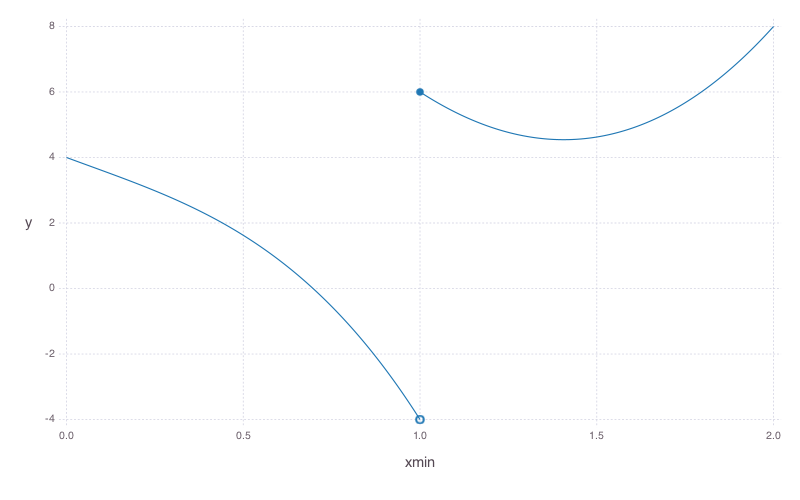
\includegraphics[width=\textwidth]{figures/allowed.png}
%         \caption{Admissible piecewise continuous function.}
%         \label{fig:allowed}
%     \end{subfigure}
%     \begin{subfigure}[t]{0.5\textwidth}\centering
%         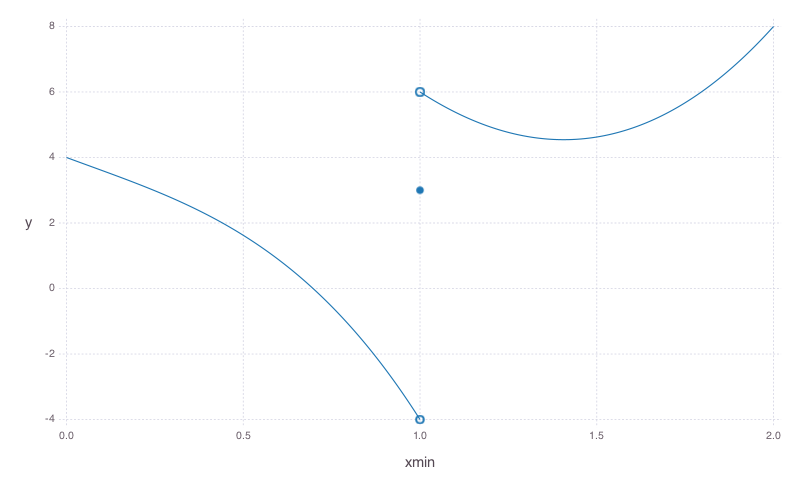
\includegraphics[width=\textwidth]{figures/not-allowed.png}
% 	    \caption{Not allowed!}
% 	    \label{fig:not-allowed}
%     \end{subfigure}
%     \caption{Examples to Definition \ref{definition-piecewise-continuous}.}
% \end{figure*}


\section{Definition DDE}
    \label{sec:definition-dde}
    % TODO: multiple fixed, discrete, bounded delay

    % TODO: also, but not here: state-dependent delay, distributed delay

    \cite{Roussel04DDEs}

    \begin{definition}[Delay Differential Equation]\label{def:dde}
        Let $f\from\deff\to\R^n$ and time delays $0<\tau_1<\ldots<\tau_k$ $\tau_j > 0$ for $j=\range{1}{k}$. Put $\taumax\defeq\tau_k\max_j\set{\tau_j}$ and $\taumin\defeq\tau_1$.

        A functional equation of the form
        \begin{equation}\label{eq:dde}
            \D{x}(t) = f(t,x(t),x(t-\tau_1),\ldots,x(t-\tau_k))
        \end{equation}
        is called (first order) \emph{delay differential equation} (DDE) with \emph{multiple constant, discrete delays $\tau_j$}.
        It is \emph{autonomous} if its right hand side $f$ is time independent and \emph{pure} if the right hand side only depends on $x(t-\tau_i)$ and not on $x(t)$.

        A DDE can be equipped with an \emph{initial condition} $x_{\tzero}$. It specifies the state, i.e.\ the values of $x$ on $[\tzero-\taumax, \tzero]$ on which the right hand side depends.
        Such a pair is called \emph{initial value problem (IVP)}:
        \begin{equation}\label{eq:ivp}
            \begin{cases}
                \D{x}(t) = f(t,x(t),x(t-\tau_1),\ldots,x(t-\tau_k)) & \text{for } t\geq\tzero\\
                x(t) = x_{\tzero}(t) & \text{for } t\in [\tzero-\taumax,\tzero]
            \end{cases}
        \end{equation}
    \end{definition}

    % Since we only consider autonomous DDEs, we can without loss of generality restrict to the case of initial time $t_0=0$.

    % The definition of a DDE can be extended to multiple constant discrete delays. For simplicity, we restrict here to a single delay.


\section{Definition of Solution}
    \label{sec:definition-of-solution}

    \begin{definition}[Solution of DDE]\label{def:solution-dde}
        A function $x\from\compactum{\tzero-\taumax}{\tzero+T}\to\R^n$ is called \emph{(local) solution} of the initial value problem~\eqref{eq:ivp}, if and only if
        $x$ is continuous and piecewise continuously differentiable on $\compactum{\tzero}{\tzero+T}$ (in the sense of Def.~\ref{def:piecewise-continuous}) with partition $\Delta$.
        This means, when $\Delta=\partition{\tzero=t_0}{t_m=\tzero+T}$, $x$ is continuously differentiable on each interval $(t_i,t_{i+1})$
        %there exists a $T>0$ such that
        % FIXME: local solution is on a single subdiv int only -> cont diffable
        %$\restrict{x}{(t_i,t_{i+1})}\in \Cn[1]{\compactum{\tzero}{\tzero+T}}{\R^n}$ with
        with
        \begin{equation*}
            \D{x}(t) = f(t,x(t),x(t-\tau_1),\ldots,x(t-\tau_k))
        \end{equation*}
        for all $t\in (\tzero,\tzero+T)$ and in $t=t_i$, it holds
        % TODO: for the right-hand derivative?
        % cf ODE sol
        \begin{equation*}
            \lim_{s\downto t_i}\D{x}(s) = f(t_i,x(t_i),x(t_i-\tau_1),\ldots,x(t_i-\tau_k))
        \end{equation*}
        and $x$ obeys the initial condition:
        \begin{equation*}
            x(t) = x_{\tzero}(t) \quad\text{for } t\in [\tzero-\taumax,\tzero].
        \end{equation*}
        % FIXME: global solution should allow knicks
        If the function $x$ is a solution for all $T>0$, it is called \emph{global}.

        %TODO: differentiable in right rand point? need not derivative in right hand point
        in knots: right sided derivative
        %TODO: Fortsetzbarkeit For example initial condition has jump, this point is limit for local solution.
    \end{definition}

\cite{Roussel04DDEs}
solution of equation is operator mapping from functions on $\compactum{t-\taumax}{t}$ to functions on $\compactum{t}{t+\taumax}$
then solution of initial value problem sequence of these functions
derivative not necessarily continuous at knots

% \begin{figure}[h]\centering
%     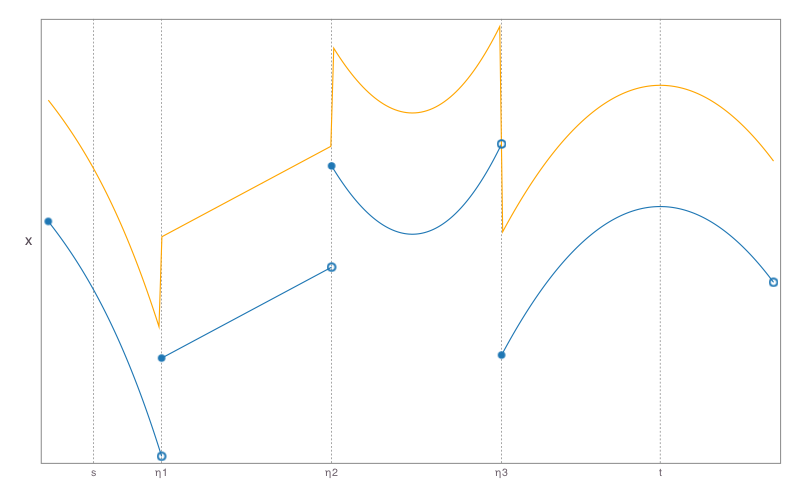
\includegraphics[width=\textwidth]{figures/multiple.png}
% 	\caption{Illustration of proof to Lemma \ref{lemma-continuity}}
% 	\label{fig:not-allowed}
% \end{figure}

% FIXME: This lemma is wrong. Show instead integrability of f(t,x_t)
\begin{lemma}
    \label{lemma-continuity}

    % Let $x:[\tzero-\tau,\tzero+T] \rightarrow \R^n$ be piecewise continuous (as in Definition \ref{definition-piecewise-continuous}) with the partition $\{t_0,\ldots,t_k\}$, i.e. there are $k$ subintervals.
    %
    % Then $t \mapsto x_t = x(t+\theta)$, where $\theta\in[-\tau,0]$, is a piecewise continuous mapping from $[\tzero,\tzero+T]$ into $\statespace[\tau]$.
\end{lemma}

\begin{proof}
    % $x$ is piecewise continuous and hence uniformly piecewise continuous on the compact interval $I=[\tzero-\tau,\tzero+T]$.
    % i.e. uniformely continuous on each subinterval with stetiger Fortsetzung in right side.
    % \begin{equation}
    %     \forall\epsilon >0 \exists\delta_i >0 \forall t,s\in I_i: \quad \abs{t-s}<\delta_i \Rightarrow \nnorm{x(t)-x(s)}<\epsilon
    % \end{equation}
    % Let $\epsilon > 0$. $x|_{[t_i,t_{i+1}]}$ (with stetiger fortsetzung in right interval limit) is uniformly continuous, i.e. there is a $\delta_i > 0$ (for the given $\epsilon$), such that $\forall\,t, s \in [t_i,t_{i+1}]$ holds
    % % TODO: can use \leq ?
    % \begin{equation}
    %     \abs{t-s} < \delta_i \Rightarrow \nnorm{x(t)-x(s)} < \epsilon
    % \end{equation}
    %
    % Among the given $\delta_i$, choose the smallest as $\delta = \min_i \delta_i$.
    %
    % For any $i$ and $s,t\in [t_i,t_{i+1})\subset [\tzero,\tzero+T]$ with $\abs{t-s}<\delta$, it holds
    % \begin{equation}
    %     \supnorm{x_t - x_s} = \sup_{\theta\in [-\tau,0]}\nnorm{x(t+\theta) - x(s+\theta)} < \epsilon
    % \end{equation}
    % since $t+\theta, s+\theta \in I$
    % Hence $t \mapsto x_t$ is uniformely continuous on $[t_i,t_{i+1})$.
\end{proof}


\section{Method of Steps}
    \label{sec:method-of-steps}
    
    See \cite{Falbo06FDEs}
    by restricting the IVP onto an interval
    actually have an ODE IVP
    convert DDE into a ODE on a certain interval, by plugging the given initial condition into the delay differential equation, eliminating the explicit dependance on the past
    can be repeated on next interval by inserting the previously computed solution instead of the initial condition

    for $t\in [0,\tau]$, $x$ must satisfy the following ordinary initial value problem obtained by plugging the initial function into equation (??). For suitable $f$ and $x_0$, the existence (and uniqueness) of a solution on $[0,\tau]$ is guaranteed by ODE theory (\ldots{} or Picard-Lindelöf theorems).

    This procedure can then be applied repeatedly to extend the obtained solution by steps of length $\tau$.





\section{Existence and Uniqueness of Solutions}
    \label{solutions-existence-uniqueness}

    cannot have more than one solution
    under certain conditions, there is such 

    will consider rhs cont and lip
    $f$ Lipschitz with piecewise continuous initial function have existence and uniqueness ???? smoothing

    \begin{definition}[Lipschitz Continuity]\label{def:lipschitz}
        % similar to \cite{pruesswilke10GewDiffGl,Smith10IntroDDE}
        % FIXME: dont I need xtau in right side ??? 
        A function $f\from\deff\to\R^n$ is called \emph{(locally) Lipschitz continuous} (in its $i$-th argument) if and only if for all $a,b\in\R$ and $M>0$ there is a $L>0$ such that
        \begin{equation*}
            % TODO: is L(\nnorm*{x-x}+\nnorm*{y-y}) better? is equiv, with different L
            % FIXME: or just say Lipschitz continuous with respect to two other arguments, once for x once for y -> compare proof
            \nnorm*{f(t,x_1,\ldots,x_i,\ldots,x_k) - f(t,x_1,\ldots,y_i,\ldots,x_k)} \leq L\nnorm*{x_i - y_i}
        \end{equation*}
        for all $t\in [a,b]$ and $x_j,y_i\in\R^n$ with $\nnorm{x_j},\nnorm{y_i},\leq M$.
    \end{definition}

    \begin{lemma}\label{lm:bounded-lipschitz}
        Let $f\from\deff\to\R^n$ be continuous and Lipschitz continuous in all but its first argument.

        For any given compact interval $\compactum{a}{b}$ and $M>0$ there exists a bound $K>0$ such that
        \begin{equation}
            \nnorm{f(t,x_1,\ldots,x_k)}\leq K
        \end{equation}
        for all $t\in\compactum{a}{b}$ and $x_j\in\R^n$ with $\nnorm{x_j}\leq M$.
    \end{lemma}
    \begin{proof}
        Let $L_i$ be the Lipschitz constant for the $i$-th argument of $f$ on the given $\compactum{a}{b}$ and $M$. Set $L\eqdef\max_i\set{L_i}$. Then
        \begin{multline*}
            \nnorm{f(t,x_1,\ldots,x_k)} \leq \nnorm{f(t,x_1,\ldots,x_k) - f(t,0,\ldots,0)} + \nnorm{f(t,0,\ldots,0)}\\
            \leq L_i\nnorm{x_i-0} + \nnorm{f(t,0,\ldots,0)} \leq LM+P = K
        \end{multline*}
        for $t\in\compactum{a}{b}$ and $x_j\in\R^n$ with $\nnorm{x_j}\leq M$. We used the continuity of $f$ on the compact set $\compactum{a}{b}$ for the existence of
        \begin{equation*}
            P = \max_{s\in\compactum{a}{b}}\nnorm{f(s,0,\ldots,0)}
        \end{equation*}
    \end{proof}

    \begin{lemma}\label{lm:integral-equation}
        %TODO: compare with ODE lecture notes
        Finding a solution of the initial value problem~\eqref{eq:ivp} is equivalent to solving the integral equation
        \begin{equation*}\label{eq:integral-equation}
            \begin{cases}
                x(t) = x_{\tzero}(\tzero) + \integral{\tzero}{t} f(s,x(s),x(s-\tau_1),\ldots,x(s-\tau_k))\dx[s] & \text{for } t\geq\tzero\\
                x(t) = x_{\tzero}(t) & \text{for } t\in [\tzero-\taumax,\tzero]
            \end{cases}
        \end{equation*}
        where ... (same as for ivp)
        and is continuous in t.
        integral componentwise, f vector valued
    \end{lemma}
    \begin{proof}
        Let $x$ be a solution of the IVP. Thus $x$ is (by definition) piecewise continuous on $\compactum{\tzero-\taumax}{\tzero}$ andcontinuous and piecewise continuous differentiable on $\compactum{\tzero}{\tzero+T}$ with piecewise derivative $f(t,x(t),x(t-\tau_1),\ldots,x(t-\tau_k))$. This chain of a piecewise continuous and continuous function is piecewise continuous and hence by Lemma~\ref{lm:pc-integrable} integrable on $\compactum{\tzero}{\tzero+T}$.

        By Lemma~\ref{lm:pc-hauptsatz} it follows
        \begin{equation*}
            x(t) = x_{\tzero}(\tzero) + \integral{\tzero}{t} f(s,x(s),x(s-\tau_1),\ldots,x(s-\tau_k))\dx[s]
        \end{equation*}
        for $t\geq\tzero$.

        Conversely, let $x$ be a solution of the integral equation~\eqref{eq:integral-equation}.
        By the the fundamental theorem of calculus is $x$ continuous on $\compactum{\tzero}{\tzero+T}$ and differentiable in $t\in\compactum{\tzero}{\tzero+T}$ if $s\mapsto f(s,x(s),x(s-\tau_1),\ldots,x(s-\tau_k))$ is continuous in $s=t$.

         has the partition
        We define a partition of $\compactum{\tzero}{\tzero+T}$ by
        \begin{equation*}
            \mathcal{Z}\defeq\set{\tzero,\tzero+T}\cup\bigcup_{j=1}^{k}\bigcup_{\substack{i=1\\t_i\geq\tau_j}}^{m}\set{t_i-\tau_j}\defeq\partition{\hat{t}_0}{\hat{t}_p}
        \end{equation*}
        If $s\in\open{\hat{t}_{l-1}}{\hat{t}_l}$ then is $s-\tau_j\neq t_i$ for all $j$ and $i$. Hence the mapping $t\mapsto f(t,x(t),x(t-\tau_1),\ldots,x(t-\tau_k))$ is continuous in $t=s$, what implies that $x$ is differentiable in $s$ and that $\D{x}(s)=f(s)$.

        \begin{align*}
            \lim_{s\downto\hat{t}_l} \D{x}(s)
            &= \lim_{s\downto\hat{t}_l} f(s,x(s),x(s-\tau_1),\ldots,x(s-\tau_k))\\
            &= f(\hat{t}_l,x(\hat{t}_l),x(\hat{t}_l-\tau_1),\ldots,x(\hat{t}_l-\tau_k))
        \end{align*}
        by the continuity of $f$ and $\lim_{s\downto\hat{t}_l} x(s-\tau_j) = x(\hat{t}_l-\tau_j)$
        the limits exist
        \begin{equation*}
            \lim_{s\upto\hat{t}_l} \D{x}(s) = \lim_{s\upto\hat{t}_l} f(s,x(s),x(s-\tau_1),\ldots,x(s-\tau_k)) = 
        \end{equation*}
        Obviously, it obeys the initial condition, i.e. $x(t)=x_{\tzero}(t)$ for all $t\in\compactum{\tzero-\tau}{\tzero}$.
        % FIXME: f cont uberall in Voraussetzung?
    \end{proof}

    \begin{theorem}[Existence of unique solution]\label{thm:solution-existence}
        Consider the Delay Differential Equation
    %TODO: do we need global existence or just local?
        \begin{equation}
            \begin{cases}
                \D{x} = f(t,x(t),x(t-\tau)) & \text{for } t\geq\tzero\\
                x(t) = x_\tzero(t-\tzero)   & \text{for } t\in [\tzero-\tau,\tzero]
            \end{cases}
        \end{equation}
        with $f\from\deff\to\R^n$ continuous and satisfying the (local) Lipschitz condition in its second argument (Def.~\ref{def:lipschitz}).

        % where $\nnorm{\cdot}$ denotes the Euclidian norm on $\R^n$ and $\supnorm{\cdot}$ the supremum norm of the Banach space of continuous functions on $[-\tau,0]$.

        Then for each \emph{initial condition} $x_{\tzero}\in\statespace[\tau]$ and start time $\tzero$, there \textbf{exists} a \textbf{unique local solution} of the IVP on a time interval $[\tzero-\tau, \tzero+T]$. The duration $T>0$ depends on the sup-norm and discontinuity points of the initial condition. (?)
        This solution is continuous and piecewise differentiable on $\compactum{\tzero}{\tzero+T}$ with partition $t_i+\tau$.
    \end{theorem}

    The proof is smiliar to the proof of the existence theorem (Theorem 3.7) given in~\cite{Smith10IntroDDE}.
    \begin{proof}
        % FIXME: where sup-norm?
        As a piecewise continuous function, the initial condition can bounded by $M\geq \supnorm{x_\tzero}$ on $\delayinterval[-\tau]$.
        
        % FIXME: do I need t_0+tau or is just \tau okay? do I need x not to be pw, just cont in proof?
        If $\set{\range{-\tau=t_0}{t_k=0}}$ is the partition of $x_{\tzero}$, we choose $T=\min\set{t_0+\tau,\frac{M}{K}}$.
        
        % FIXME: M or 2M?
        Let $K>0$ be the upper bound for $f$ from Lemma~\ref{lm:bounded-lipschitz} on the set $S=[\tzero,\tzero+T] \times \{x\in R^n: \nnorm{x}\leq 2M\}\times \{y\in R^n: \nnorm{y}\leq 2M\}$ and $L>0$ the Lipschitz constant of $f$ for that set.

        % FIXME: why continuous? its pw cont? cont in tzero
        We construct a series $(x_{(m)})_{m\in\N_0}$ of piecewise continuous functions which approximates the solution of the initial value problem.
        Set
        \begin{equation}
            x_{(0)}(t)= \begin{cases}
                x_\tzero(0) & t\in [\tzero,\tzero+T]\\
                x_\tzero(t-\tzero) & t\in [\tzero-\tau,\tzero]
            \end{cases}
        \end{equation}
        For $m\in\N_{>0}$ define
        \begin{equation}
            x_{(m)}(t)= \begin{cases}
                x_\tzero(0) + \int_\tzero^t f(s,x_{(m-1)}(s),x_{(m-1)}(s-\tau))\dx[s] & t\in [\tzero,\tzero+T]\\
                x_\tzero(t-\tzero) & t\in [\tzero-\tau,\tzero]
            \end{cases}
        \end{equation}
        % FIXME: why exists integral? f cont, x in int even cont
        Integral exists
        It holds for all $m>0$ and $t\in \compactum{\tzero-\tau}{\tzero}$ by definition of the series
        \begin{equation}
            \nnorm*{x_{(m)}(t)-x_{(m-1)}(t)}=0
        \end{equation}
        We show by induction over $m$ that for all $t\in [\tzero,\tzero+T]$ it holds
        \begin{equation}
            \nnorm*{x_{(m)}(t)-x_{(m-1)}(t)} \leq \frac{K}{L}\frac{L^m (t-\tzero)^m}{m!}.
        \end{equation}
        Since obviously $\nnorm{x_{(0)}(t)}\leq M$, the statement for $m=0$ follows from the boundedness of $f$ on $S$ and the triangle inequality for integrals:
        \begin{equation}
            \nnorm{x_{(1)}(t)-x_{(0)}(t)} = \nnorm*{\int_\tzero^t f(s,x_{(0)}(s),x_{(0)}(s-\tau))\dx[s]} \leq K(t-\tzero)
        \end{equation}
        In the inductive step we can apply
        Since for any $m>0$, it holds by the triangle inequality and by the choice of $T$
        % FIXME: why x(m)(t) smaller than 2M, such that K holds?
        % TODO: why do integral and norm commute? once integral over vectors, once over scalars
        \begin{align}\label{eq:bounded-xm}
            \nnorm*{x_{(m)}} &\leq \nnorm*{x_\tzero(0)} + \int_\tzero^t \nnorm*{f(s,x_{(m-1)}(s),x_{(m-1)}(s-\tau))}\dx[s]\\
            &\leq M + K(t-\tzero) \leq M+KT\\
            &\leq 2M
        \end{align}
        if $\nnorm{x_{(m-1)}(t)}\leq 2M$.
        It follows by the Lipschitz property of $f$
        \begin{multline*}
            \nnorm*{x_{(m+1)}(t)-x_{(m)}(t)}=\\
            = \nnorm*{\int_\tzero^t f(s,x_{(m)}(s),x_{(m)}(s-\tau)) - f(s,x_{(m-1)}(s),x_{(m-1)}(s-\tau))\dx[s]}\\
            \leq L \int_\tzero^t \nnorm*{x_{(m)}(s) - x_{(m-1)}(s)}\dx[s]\\
            \leq \frac{L^m K}{m!} \int_\tzero^t (s-\tzero)^m\dx[s]
            = \frac{L^m K}{(m+1)!}(t-\tzero)^{m+1}
        \end{multline*}
        %We use this bound and the triangle inequality in
        The Cauchy criterion for convergent series (\cite{Gathmann12GDM} 6.13, \cite{Rudin76PrinciplesAnalysis} 3.22) applied to the exponential series states that
        \begin{equation*}
            % "\ " needed for space
            \mforall{\epsilon>0}\ \mexists{n_0\in\N_0}\ \mforall{m\geq k\geq n_0}\holds \sum_{i=k+1}^m \frac{(LT)^i}{i!} <\epsilon
        \end{equation*}
        So for any $\epsilon>0$ exist $k\in\N_0$ and $m\geq k$, such that
        \begin{align*}
            \nnorm*{x_{(m)}(t)-x_{(k)}(t)} \leq{} & \nnorm*{x_{(m)}(t)-x_{(m-1)}(t)} + \nnorm*{x_{(m-1)}(t)-x_{(m-2)}(t)} + {}\\
            & + \ldots + \nnorm*{x^{(k+1)}(t)-x^{(k)}(t)}\\
            \leq{} & \frac{K}{L}\frac{L^m (t-\tzero)^m}{m!} + \frac{K}{L}\frac{L^{m-1} (t-\tzero)^{m-1}}{(m-1)!} + {}\\
            & + \ldots +\frac{K}{L}\frac{L^{k+1} (t-\tzero)^{k+1}}{(k+1)!}\\
            \leq{} & \frac{K}{L}\sum_{i=k+1}^m \frac{(LT)^i}{i!} < \varepsilon
        \end{align*}
        for all $t\in [\tzero,\tzero+T]$, i.e. $x_{(m)}$ is a Cauchy sequence

    
        % FIXME: show that this a Cauchy series
        %This is the tail of the convergent exponential series and hence it converges to zero for $k\to\infty$ (boundedness and positivity of summands, monotonicity crit).

        % FIXME: why continuous? since integral exists
        Since $x_{(m)}$ is continuous on $[\tzero,\tzero+T]$, this Cauchy
        sequence admits a limit $x$ in the Banach space $\continuouss[0]{[\tzero,\tzero+T]}{\R^n}$ in terms of the supremum-norm.

        Again, we extend $x$ to $[\tzero-\tau,\tzero]$ with $x_\tzero$, such that $x\in\Cnpw[0]{[\tzero-\tau,\tzero]}{\R^n}$.


        

        Since by the continuity of the supremum norm it follows from~\eqref{eq:bounded-xm} that
        \begin{equation*}
            \supnorm*{x}=\lim_{m\to\infty}\supnorm*{x_m}\leq 2M
        \end{equation*}
        can apply Lipschitz property of $f$
        \begin{equation*}
            \sup_{t\in\compactum{\tzero}{\tzero+T}}\nnorm*{f(s,x_m(s),x_m(s-\tau))-f(s,x(s),x(s-\tau))} \leq \sup_{t\in\compactum{\tzero}{\tzero+T}}\nnorm*{x_m(t)-x(t)}
        \end{equation*}
        Due to the uniform convergence (conv in sup-norm) of $x_{(m)}\to x$, we get the uniform convergence
        \begin{equation*}
            f(s,x_m(s),x_m(s-\tau)) \xrightarrow{m\to\infty} f(s,x(s),x(s-\tau))
        \end{equation*}
        and hence the integral and the limit process swap and by
        \begin{align*}
            x(t) = \lim_{m\to\infty} x^{(m+1)} &= x_\tzero(0) + \lim_{m\to\infty}\int_\tzero^t f(s,x^{(m)}(s),x^{(m)}(s-\tau))\dx[s]\\
            &= x_\tzero(0) + \int_\tzero^t f(s,x(s),x(s-\tau))\dx[s]
        \end{align*}
        it follows that $x$ solves the integral equation and hence, by Lemma~\ref{lm:integral-equation},
        this proves the existence of a solution to the DDE.
        % TODO: continuous because limit in Banach space, diffable and subdiv see integral equiv lemma

        % TODO: can one solution be on [\tzero, T_2] with T_2<T ?
        It remains to show uniqueness.
        Let $x$ and $\bar{x}$ be two solutions of the DDE on $[\tzero,\tzero+T]$.
        By Lemma \ref{lm:integral-equation} they are equivalent to solutions of the integral equations
        \begin{equation}
            x(t) = x_\tzero(0) + \int_\tzero^t f(s,x(s),x(s-\tau))\dx[s]
        \end{equation}
        and
        \begin{equation}
            \bar{x}(t) = x_\tzero(0) + \int_\tzero^t f(s,\bar{x}(s),\bar{x}(s-\tau))\dx[s]
        \end{equation}
        For $t\in [\tzero,T]$, we set
        \begin{align*}
            \rho(t) &:= \nnorm*{x(t)-\bar{x}(t)} \leq \int_\tzero^t \nnorm*{f(s,x(s),x(s-\tau))-f(s,\bar{x}(s),\bar{x}(s-\tau))}\dx[s]\\
            & \leq L \int_\tzero^t \nnorm*{x(s)-\bar{x}(s)}\dx[s] = L \int_\tzero^t \rho(s)\dx(s)\\
            &= L \int_\tzero^t \e{-\alpha s}\rho(s)\e{\alpha s}\dx[s] \leq L \sup_{s\in [\tzero,\tzero+T]}\left(\e{-\alpha s}\rho(s)\right)\int_\tzero^t \e{\alpha s}\dx[s]\\
            & \leq\frac{L}{\alpha}\e{\alpha t} \sup_{s\in [\tzero,\tzero+T]}\left(\e{-\alpha s}\rho(s)\right)
        \end{align*}
        with $L$ the Lipschitz constant of $f$ on the set ...
        and $\rho$ is continuous, since $x$ continuous
        Choosing $\alpha=2L$ and multiplying with $\e{-\alpha t}>0$ leads to
        \begin{equation}
            \rho(t)\e{-2Lt} \leq \frac{1}{2}\sup_{s\in [\tzero,\tzero+T]}\left(\e{-2L s}\rho(s)\right)
        \end{equation}
        for all $t\in [\tzero,\tzero+T]$
        \begin{equation}
            0 \leq \sup_{t\in [\tzero,\tzero+T]}\left(\rho(t)\e{-2Lt}\right) \leq \frac{1}{2}\sup_{s\in [\tzero,\tzero+T]}\left(\e{-2L s}\rho(s)\right)
        \end{equation}
        That is only possible if $\rho(t)=0$ for all $t\in [\tzero,\tzero+T]$, which means $x(t)=\bar{x}(t)$.

        % TODO: still needed?
        just proof existence/uniqueness on each peace of continuity proof continuity at knots with Lemma of integral equ

    \end{proof}

% TODO: on [\tzero,t_1] DDE equiv to ODE/IntEq
% -> ex unique sol on [\tzero, t_1]
% -> ex unique sol on [\tzero,\tau] (glob Lip of f on [tzero,tau])
% -> ex unique sol on [\tzero,2\tau] (continuous?, diffable?)
% show continuity and pw diffable (nth to show)
    % \begin{lemma}[cont]\label{lm:c}
    %     $x_1$ loc sol on $\compactum{\tzero-\tau}{\tzero+t_1}$ for init cond $x_{\tzero}$
    %     $x_2$ and loc sol on $\compactum{\tzero+t_1-\tau}{\t_1+T}$ for init cond $x_1$
    %     then $x_1(\tzero+t_1)=x_2(\tzero+t_1)$
    %     follows from initial cond $x_1$
    % \end{lemma}
\begin{corollary}
    \label{cor:continuability-of-solution}

    % TODO: What is derivation in randpunkten of interval [] ?
    If in Theorem \ref{theorem-solution-existence} $T=t_1-\tau$, can reapplay theorem with starting point $\tzero=\tzero_{old}+t_1-\tau$. Get existence of unique solution on $[\tzero-\tau,\tzero+S]$ with $S>T$.
\end{corollary}

\begin{corollary}
    \label{corollary}
    If f is polynomial in $t$, $x(t)$ and $x(t-\tau)$ then theorem holds

    polynomial -> continuously differentiable -> locally Lipschitz
% IDEA: can show? init cond bounded by M, and loc sol bounded by M, get glob sol since f glob Lip on set of bounded inputs?


    %TODO: put after uniqueness theorem, need uniqueness and existence so that amap well-defined
    The notion of solution for an autonomous DDE as given above can be lifted to be a trajectory $\trajectory[x]$ in the statespace
    \begin{equation}
        \trajectory[x] \from [0,T] \to \statespace[\tau],\\
        t \mapsto \xbartaut{t}
    \end{equation}

    The \emph{state} at time $t$ is a function which provides a time limited history up to the current time. This is all information needed to determine (using the DDE) to determine the solution for time $\geq t$. It is defined as $\xbartaut{t}(s)\defeq x(t+s)$ for $s\in [-\tau,0]$. In the case of $t=0$, we simplify the notation to $\xbartau \defeq \xbartaut{0}$.
    This notion of solution is a \emph{dynamical systems} point of view which later turns out to be useful.

  Other results know from ordinary differential equations can be adapted to delay differential equations, such as continuous (or even differentiable) dependence of the solution on initial data and, see \cite{Dads06DDEs} % TODO: add other cites

%TODO: can write DDE (eq??) from definition as

\begin{equation}
    \begin{cases}
        \D{x}=f(\xbartaut{t})\defeq g(\xbartaut{t}(0),\xbartaut{t}(-\tau)) &\text{for } t\geq 0\\
        x(t)=x_0(t) & \text{for } t\in[-\tau,0]
    \end{cases}
\end{equation}
\end{corollary}

\begin{proof}

\end{proof}

% TODO: non-autonomous -> autonomous

\begin{example}
    Delay differential equations can often incorporate a much richer behaviour than ordinary differetial equations.
    The basic ODE IVP
    \begin{equation}
        \begin{cases}
            \D{x}(t) = -x(t)\\
            x(0) = x_0
        \end{cases}
    \end{equation}
    has the solution $x(t)=x_0 e^{-t}$. However the similiar DDE
    \begin{equation}
        \begin{cases}
            \D{x}(t) = -x(t-\tau) & t\geq 0\\
            x(t) = x_0(t) & -\tau\leq t\leq 0
        \end{cases}
    \end{equation}
    has a much richer dynamics, but solution (as series) for $x_0\equiv 1$, can compute first solutions by method of steps. \ldots{}    
\end{example}


\begin{figure}[h]\centering
    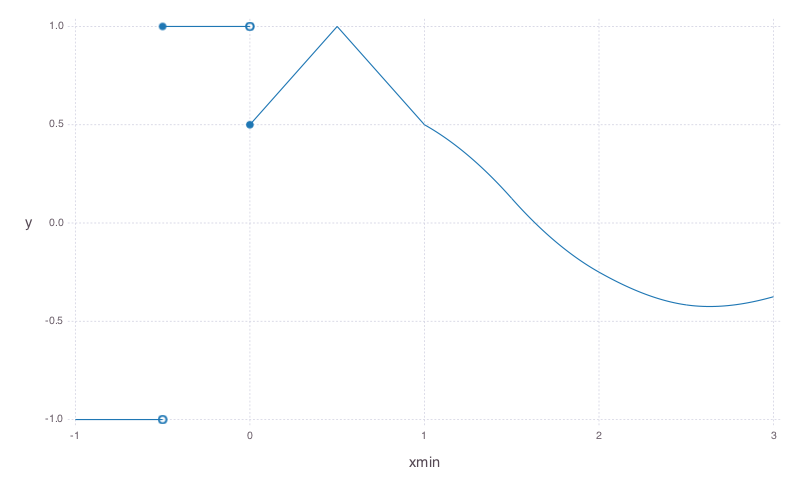
\includegraphics[width=\textwidth]{figures/piecewise-initial-function.png}
	%\caption{}
	\label{fig:not-allowed}
\end{figure}



\chapter{Delay Differential Dynamic Logic}
\label{ch:delay-differential-dynamic-logic}

We extent classical differential dynamic logic (\dL) (see e.g.~\cite{Platzer12LogicsDynSys}) with syntax, semantics, axiomatization and proof rules to support reasoning about hybrid dynamical systems with delay.

To that purpose, we allow delay differential equations in hybrid programs, which are then called \emph{delay hybrid program} (\dHP).

The definition of \emph{delay differential dynamic logic} (\ddL) provides all operators of first-order logic, as well as modal operators, in order to specify and verify reachability properties about the state of such \dHPs.

In the language of \ddL, we can not only model hybrid programs with DDEs in the continuous part, but also with temporal differences in the discrete fragment.
For example a controller which approximates a derivative by a difference quotient.

The logic \ddL is a superset of \dL, i.e.\ in the absence of any delay, it reduces to classical \emph{differential dynamic logic}.


% Similiar to first-order logic and essentially as an extension of dL we define delay differential logic
% in general an arbitrary unknown initial function, only conditions on it

% time-invariant

% safety and liveness properties specify

% TODO: Abgrenzung zu Trace Semantics
    % The temporal character of delay differential equations (they depend on their own temporal evolution with limited horizon) suggests the introduction of trace semantics.
    %
    % However, we go the way of introducing transition semantics with an augmented state space.

\section{Syntax}
    \label{sec:syntax}

    The syntax of \ddL terms, formulas as well as of \dHPs is defined inductively by grammars in Backus-Naur-form (BNF).

    We define by $\allvars$ be the set of \emph{all variables} and by $\diffvars\defeq\Set{\D{x} \with x\in\allvars}$ the corresponding set of \emph{differential symbols}.
    % TODO: call delay or delayed?
    % FIXME: just use \Q as set of constants, they have their semantics
    % Let $\constants$ be the set of \emph{all constants}.
    We denote $\delayvars\defeq\Set{\x[b] \with x\in\allvars,\ b\in\nonposQ}$ as the set of \emph{delay variables} and $\delaydiffvars\defeq\Set{\Dx[b] \with \D{x}\in\diffvars,\ b\in\nonposQ}$ as the set of \emph{delay differentials}.
    % TODO: finite sets, or sets infinite, but only finitely many symbols in one term/formula, Trm()
    % FIXME: parentheses

    We will usually write variables as $x,y,z\in\allvars$ and their differential symbols as $\D{x},\D{y},\D{z}\in\diffvars$.
    \emph{Function symbols} $f,g,h$ and \emph{constant symbols} $a,b,c\in\constants$
    % FIXME: do I use predicates?
    % \emph{predicate symbols} $p,q,r$
    are as in first-order logic (cf.\ Section~\ref{sec:first-order-logic}).

    Moreover, we write $\astrm,\bstrm$ for \ddL terms, $\asfml,\bsfml$ for \ddL formulas and $\asprg,\bsprg$ for \dHPs. For formulas of first-order logic of real arithmetic (\FOLR), we use the symbols $\asfmlfolR$ and $\bsfmlfolR$.

    \begin{definition}[s-Terms]\label{def:syntax-terms}
        The syntax of \emph{terms} of \emph{delay differential dynamic logic} is defined by the following grammar:
        \begin{align*}
            \astrm(s),\bstrm(s) \Coloneqq{}&
                \x[s] \mid
                \Dx[s] \mid
                \x[b] \mid
                \Dx[b] \mid
                c \mid\\
                & f(\range{\istrm{1}(s)}{\istrm{k}(s)}) \mid
                \astrm(s) + \bstrm(s) \mid
                \astrm(s) \cdot \bstrm(s) \mid
                \D{(\astrm(s))}
        \end{align*}
        % FIXME: is term' allowed? diff inv is only a FOLR formula? even for dL valid?
        % TODO: line breaks and explination text in syntax
        % \begin{align}
        %     \astrm\Coloneqq{}&\\
        %     &\mid \astrm+\bstrm\hfill\text{test}
        % \end{align}
        where $x\in\allvars,\D{x}\in\diffvars$ and $f$ is a function symbol of arity $k$.
        The symbol $c\in\constants$ stands for a constant value in $\Q$. The constant parameters $b\in\nonposQ$ are not allowed to be positive.
    \end{definition}

    The s-terms listed in the first line are called \emph{atomic}, as opposed to the \emph{composite} s-terms in the second line.
    % FIXME: what is f like?
    %extending \dL with symbols for \emph{delayed variables} and \emph{differentials}
    S-terms generally depend on the time parameter $s\in\nonposR$. This is why we write them as $\astrm(s)$.
    If a s-term $\astrm(s)$ does neither contain $\x[s]$ nor $\Dx[s]$, we say $s\notin\astrm(s)$ and abbreviate its notation to $\astrm$.
    Writing $\astrm(b)$ means that all occurences of $s$ in $\astrm(s)$ have been replaced with $b\in\nonposQ$.
    Moreover, we agree on abbreviating $\x[0]$ to $x$ and $\Dx[0]$ to $\D{x}$.
    % The variable symbol $x$ and the differential symbol $\D{x}$ are the only ones which allow explicitely mentioning this parameter. They are spelled slightly differently using square brackets as $\x[s]$ and $\Dx[s]$, respectively.
    Note that $s\notin\allvars\cup\diffvars\cup\constants$. It is a special variable symbol.

    The \emph{differential} $\D{(\astrm(s))}$ of a term $\astrm(s)$ is its syntactic (total) derivation, obtained by standard differentiation rules.
    Lemma~\ref{lm:derivations} shows the validity of these rules and that the result is again a s-term.

    Subtraction can be defined using addition and multiplication, division would also be possible, if we can exclude any division by zero. The grammar allows in particular the construction of polynomial forms.

    \begin{example}
        Let us consider the s-term
        \begin{equation*}
            \astrm(s) = \x[s] + \x[-\tau].
        \end{equation*}
        Setting $s=-1$ gives the term
        \begin{equation*}
            \astrm(-1) = \x[-1] + \x[-\tau].
        \end{equation*}
    \end{example}

    Delay differential dynamic logic uses hybrid programs with delay differential equations as system model. 
    The grammar defining these \emph{delayed hybrid programs} is the same as for classical \HPs (cf.~\cite{Platzer15Uniform}).

    \begin{definition}[Delay Hybrid Programs]\label{def:syntax-HP}
        The syntax of \emph{delay hybrid programs} (\dHPs) is defined by
        % TODO: first-order logic of real arithmetic formulas include \x?
        \begin{equation*}
            \asprg,\bsprg \Coloneqq
                \hupdate{\humod{x}{\astrm}} \mid
                \Dupdate{\Dumod{\D{x}}{\astrm}} \mid
                \htest{\asfmlfolR} \mid
                \hchoice{\asprg}{\bsprg} \mid
                % TODO: replace ; in HPs
                \asprg;\bsprg \mid
                \hrepeat{\asprg} \mid
                \hevolvein{\D{x}=\astrm}{\ivr}
        \end{equation*}
        where $\asprg,\bsprg$ denote \dHPs, $x$ a variable and $\astrm$ a term (possibly containing $x$ or $\x[b]$, but no $\x[s]$).
        The formula $\asfmlfolR$ is of \FOLR, containing only normal variable symbols from $\allvars$.
    \end{definition}
    
    Note that the syntax only allows autonomous DDEs, though with multiple constant delays.

    Atomic \dHPs are given by instantaneous discrete \emph{assignments} $\hupdate{\humod{x}{\astrm(0)}}$ and \emph{differential assignments} $\Dupdate{\Dumod{\D{x}}{\astrm(0)}}$, which change the value of the given variable only at the current time instant, not the past, \emph{tests} $\htest{\asfmlfolR}$, which pass only if the current state satisfies first-order formula $\asfmlfolR$ of real arithmetic and abords the program execution if not, as well as evolutions along \emph{delay differential equation} systems $\hevolvein{\D{x}=\astrm(0)}{\ivr}$ of an arbitrary amount of time, but restricted by the evolution domain constraint $\ivr$.

    Compound \dHPs combine atomic programs, and comprise \emph{nondeterministic choices} $\hchoice{\asprg}{\bsprg}$, running either $\asprg$ or $\bsprg$, \emph{sequential compositions} $\asprg;\bsprg$, executing $\bsprg$ after $\asprg$ and \emph{nondeterministic repetitions} $\hrepeat{\asprg}$, repeating $\asprg$ any number of times, zero times included.

% Using this, in comparison to \dL extended syntax, we can write down both delay differential equations and ordinary differential equations in the form $\D{x}=\theta$, where $\theta=f(x,\x[-\tau])$ with a polynomial $f$.
    Observe that ODEs are still expressible by this syntax and that hybrid programs are hence only delayed hybrid programs with zero delay.

    % FIXME: where put general dL sources? only once at beginning
    The difference between classical \HPs (as defined in \dL, cf.~\cite{Platzer10HybridSystems,Platzer12LogicsDynSys,Platzer15Uniform}) and \emph{delay hybrid programs} is not syntactical, but only given by their semantics.
    
    \begin{definition}[s-Formulas]\label{def:syntax-formula}
        The syntax for \emph{formulae} of \emph{delay differential dynamic logic} is defined by the grammar
        \begin{align*}
            \asfml(s),\bsfml(s) \Coloneqq{}& % fixes missing space
                % TODO: better abbreviated notation for \holdssince, make forall only appear in semantics rhs
                \astrm(s) = \bstrm(s) \mid
                \astrm(s)\geq\bstrm(s) \mid
                p(\range{\istrm{1}(s)}{\istrm{k}(s)}) \mid
                \hs{\asfml(s)} \mid\\
                &\lnot\asfml(s) \mid
                \asfml(s)\land\bsfml(s) \mid
                \lforall{x}{\asfml(s)} \mid
                \lexists{x}{\asfml(s)} \mid
                \dbox{\asprg}{\asfml(s)} \mid
                \ddiamond{\asprg}{\asfml(s)}
        \end{align*}
        with $\astrm(s),\bstrm(s),\range{\istrm{1}(s)}{\istrm{k}(s)}$ as s-terms, $p$ as predicate symbol, $x$ as variable, and $\asprg$ as \dHP.
    \end{definition}

    These formulae combine connectives of propositional logic with first-order quantifiers (which both have standard meaning) and two modalities, describing \emph{necessary} and \emph{possible} properties.

    The other comparison operators $<,\leq,>$ and logic connectives $\lor,\limply,\lbisubjunct$ can be defined using $=,\land,\lnot$ and are hence not explicitely mentioned in the grammar.
    Analogoulsy is $\lexists{x}{\asfml}$ expressible as $\lnot\lforall{x}{\lnot\asfml}$ and the modal formula $\dbox{\asprg}{\asfml}$ ($\asfml$ holds in the state after all runs of $\asprg$) by its dual $\ddiamond{\asprg}{\asfml}\equiv\lnot\dbox{\asprg}{\lnot\asfml}$ (there is at least one state reachable by $\asprg$ such that $\asfml$ holds).
    The quantifiers $\forall$ and $\exists$ quantify over the state space $\statespace$.
    % FIXME: was state space mentioned before?

    Like the s-terms defined above, the s-formulae depend on a time parameter $s\in\closeddelayinterval$. The symbol $T$ is a symbolic constant related to the length of the domain of the state space, which is induced by the occurence of delay symbols. Its value is defined by the static semantics and set by proof rules.
    % TODO: proof rule/axiom to set T?
    The only way to bind the variable $s$ in a formula $\asfml(s)$ is by using $\hs{\asfml(s)}$, which quantifies $s$ over the domain of the state space, except for the current time point $0$.

    We note $\asfml$ to indicate that $s$ is not a free variable of $\asfml(s)$ and $\asfml(b)$ with $b\in\nonposQ$ to express that each term $\astrm(s)$ in the formula was replaced by its corresponding $\astrm(b)$, even if it was bound by a $\hs{}$.
    % TODO: or only which is not under the scope of a \hs? at the moment I overwrite each \hs
    
    % TODO: on variables \allvars (signature)
    Formulas of first-order logic of real arithmetic constitute a subset of \ddL, i.e.\ every \FOLR formula is also a formula of delay differential dynamic logic.

    \begin{convention}
        The frequently appearing fact that $\asfml(s)$ is not only supposed to hold for $s\in\delayinterval$ but also in $s=0$
        \begin{equation*}
            \hs{\asfml(s)}\land\asfml(0)
        \end{equation*}
        can also be written as
        \begin{equation*}
            \hsc{\asfml(s)}
        \end{equation*}
        For convenience, we allow the latter, abbreviated notation, which is implicitely replaced by the former, syntactically correct version.
    \end{convention}

    In order to simplify notation by eliminating parentheses, we agree on the following
    \begin{convention}
        The operators in \ddL formulae obey the following binding priorities (from highest to lowest):
        \begin{itemize}
            \item the quantifiers $\forall,\exists$ and the modal operators $\dbox{\cdot}{},\ddiamond{\cdot}{}$ bind strongest
            \item negation $\lnot$ binds stronger than
            \item conjunction $\land$ binds stronger than 
            \item disjunction $\lor$ binds stronger than
            \item implication $\limply$ binds stronger than
            \item equivalence $\lbisubjunct$, which binds weakest.
        \end{itemize}
    \end{convention}

        % TODO: Move to static semantics
    Moreover, when a s-formula does not depend on the quantified parameter $s$, we can drop the quantifier $\hs{}$ in which this formula appears.

    \begin{example}
        Consider the two well-formed \ddL formulae:
        \begin{align*}
            &\hs{(x+\x[s]\geq 0)}\\
            &\hs{(x+\x[-\tau]\geq 0)} 
        \end{align*}
        The quantification over $s$ in the second formula can be dropped, what leads to the equivalent formula
        \begin{equation*}
            x+\x[-\tau]\geq 0.
        \end{equation*}
    \end{example}


\section{Dynamic Semantics}
    \label{sec:dynamic-semantics}

    % TODO: this is called valuation

    In this section, we give meaning to the syntax introduced above, by defining its semantics in a compositional way.

    Following the remark to the solution of a DDE (cf.\ Section~\ref{sec:definition-of-solution}), we define the \emph{state space} in \ddL as $\statespace$, the set of piecewise continuously differentiable functions on $\closeddelayinterval$, as defined in Definition~\ref{def:piecewise-continuous}.
    This means that a variable remembers a limited part of its evolution history, what demands hence an implicit notion of a underlying time.

    We denote by $\states$ the \emph{set of states}. A \emph{state} $\asstate\in\states$ is a mapping
    \begin{equation}
        \asstate \from \allvars\cup\diffvars \to \statespace
    \end{equation}
    which assigns a \emph{history} (function) to each variable and differential symbol.

    By $\modif{\asstate}{x}{y}$ we denote the state which is equal to state $\asstate$, except for the value of the variable $x$, which is set to $y\in\statespace$.

    % FIXME: modification of x in state and general specification of pw function associated to x
    %at the time $t=0$. The value of $x$ for the time before does not change.

    % FIXME: let interpretation $\interpret$ be fixed
    

    \begin{definition}[Semantics of s-terms]\label{def:sematic-terms}
        % FIXME: replace t by \tilde{s}
        The \emph{semantics} of a s-term $\astrm(s)$ in the state $\asstate\in\states$ with respect to the time instant $\past\in\closeddelayinterval$
        is a value in $\R$ and defined inductively as follows:
        \begin{enumerate}
            \item $\ivaluation{\IddL}{\x[s]} = \asstate(x)(\past)$ for a variable $x\in\allvars$
            % FIXME: need Cpw for derivatives or only \R?
            \item $\ivaluation{\IddL}{\Dx[s]} = \asstate(\D{x})(\past) \defeq \lim_{t\downto \past} \frac{\asstate(x)(t)-\asstate(x)(\past)}{t-\past}$ (except in $\past=0$)
            % for a differential symbol $\D{x}\in\diffvars$
            \item $\ivaluation{\IddL}{\x[b]} = \asstate(x)(b)$ for a variable $x\in\allvars$ 
            % \item $\ivaluation{\IddL}{\Dx[b]} = \asstate(\D{x})(b)$ for a differential symbol $\D{x}\in\diffvars$ and a constant $b\in\constants$ with $\interpret[b]\in\nonposQ$
            \item $\ivaluation{\IddL}{\Dx[b]} = \asstate(\D{x})(b) \defeq \lim_{\tilde{s}\downto b} \frac{\asstate(x)(\tilde{s})-\asstate(x)(b)}{\tilde{s}-b}$ (except in $\past=0$)
            \item $\ivaluation{\IddL}{c} = \interpret[c]$ for a constant $c\in\constants$
            \item $\ivaluation{\IddL}{f(\range{\istrm{1}(s)}{\istrm{k}(s)})} = \interpret[f](\range{\ivaluation{\IddL}{\istrm{1}(s)}}{\ivaluation{\IddL}{\istrm{k}(s)}})$ for a function symbol $f$
            \item $\ivaluation{\IddL}{\astrm(s)+\bstrm(s)} = \ivaluation{\IddL}{\astrm(s)} + \ivaluation{\IddL}{\bstrm(s)}$
            \item $\ivaluation{\IddL}{\astrm(s)\cdot\bstrm(s)} = \ivaluation{\IddL}{\astrm(s)} \cdot \ivaluation{\IddL}{\bstrm(s)}$
            % FIXME: derivation of terms with x'?
            \item $\ivaluation{\IddL}{\D{(\astrm(s))}} = \displaystyle\sum_{\x[b]\in\delayvars} \asstate(\D{x})(\interpret[b])\frac{\partial\ivaluation{\IddL}{\astrm(s)}}{\partial \x[b]} + \asstate(\D{x})(\past)\frac{\partial\ivaluation{\IddL}{\astrm(s)}}{\partial \x[s]}$
        \end{enumerate} 
        where $b\in\nonposQ$ is a non-positive rational number.
    \end{definition}
        % FIXME: interpretation of $f$ is a smooth function?

    The meaning of the variable and differential symbols is determined by the state. Additionally, the value of a differential symbol has to coincide with the right derivative of the corresponding variable, except for $\past=0$.

    The meaning of the differential of an arbitrary term is the total derivative of its value with respect to the underlying continuous time.
    As a composition of smooth functions is $\ivaluation{\IddL}{\astrm(s)}$ smooth itself and hence these derivatives exist.
    The sum is finite, since each term only mentions finitely many variables.

    % The meaning of a differential symbol: defined by state, 
    % The time derivative of a variable may not be defined in isolated state, because it might have a discontinuity here and we cannot use its history (provided by the state) to define derivative.
    % However, we can define a state local semantics for a differential $\D{(\astrm)}$.

    % Like for ODE case, only use last value given in state. Since in $t=0$ could be incontinuity 

    

    % Along a solution of a DDE $\varphi:[0,r]\rightarrow\states$ (continous differentiable), the differential symbols are interpreted as time derivatives, $r>0$ at any $\zeta\in[0,r]$, meaning of symbol is rate of change of value of $x$ over time
    % \begin{equation}
    %     % TODO: replace \DD with Andres command
    %     \imodel{\IddL}{\D{x}}\varphi(\zeta)
    %         = \varphi(\zeta)(\D{x})(0)
    %         \defeq \DD{\varphi(t)(x)(0)}{t}(\zeta)
    %         = \DD{\imodel{\IddL}{x}\varphi(t)}{t}(\zeta)
    % \end{equation}
   
 
    

    In the precondition, no values are associated to the differential symbols. In general, the initial function is only piecewise continuous.
    Since for later time instances, the values of the differential symbols derive from the DDE, they become (locally) smooth function.

    \begin{definition}[Semantics of s-formulae]\label{def:semantic-formulae}
        The semantics of a \ddL formula $\asfml$ is the subset of all states $\imodel{\IddL}{\asfml}\subseteq\states$ in which $\asfml$ is true. This set is given inductively by
        % TODO: mention interpretation I
        % FIXME: what is difference between \imodel and \ivaluation?
        % terms: ivaluation, formula: imodel, programms: ireachability
        % FIXME: display assign for formula semantics
        \begin{enumerate}
            % TODO: replace : in set by \with
            % FIXME: use notation forall ... : ...
            % FIXME: *version for lforall without parentheses
            % FIXME: forall quantifies over state space or over possible values (reals) for system parameters?
            \item $\imodel{\IddL}{\astrm(s)=\bstrm(s)} = \Set*{\asstate\in\states \with \ivaluation{\IddL}{\astrm(s)} = \ivaluation{\IddL}{\bstrm(s)}}$
            \item $\imodel{\IddL}{\astrm(s)\geq\bstrm(s)} = \Set*{\asstate\in\states \with \ivaluation{\IddL}{\astrm(s)}\geq\ivaluation{\IddL}{\bstrm(s)}}$
            \item $\imodel{\IddL}{p(\range{\istrm{1}(s)}{\istrm{k}(s)})} = \Set*{\asstate\in\states \with \left(\range{\ivaluation{\IddL}{\istrm{1}(s)}}{\ivaluation{\IddL}{\istrm{k}(s)}}\right)\in\interpret[p]}$
            \item $\imodel{\IddL}{\lnot\asfml(s)} = \scomplement{\left(\imodel{\IddL}{\asfml(s)}\right)} = \states\setminus\imodel{\IddL}{\asfml(s)}$
            \item $\imodel{\IddL}{\asfml(s)\land\bsfml(s)} = \imodel{\IddL}{\asfml(s)}\cap\imodel{\IddL}{\bsfml(s)}$
            \item $\imodel{\IddL}{\hs{\asfml(s)}} = \Set*{\asstate\in\states \with \mforall{\tilde{r}\in\delayinterval}\holds\asstate\in\imodel{\iconcat[assign=\tilde{r}]{\IddL}}{\asfml(s)}}$
            \item $\imodel{\IddL}{\lforall{x}{\asfml(s)}} = \Set*{\asstate\in\states \with \modif{\asstate}{x}{y}\in\imodel{\IddL}{\asfml(s)} \text{ for all } y\in\statespace}$
            \item $\imodel{\IddL}{\lexists{x}{\asfml(s)}} = \Set*{\asstate\in\states \with \modif{\asstate}{x}{y}\in\imodel{\IddL}{\asfml(s)} \text{ for some } y\in\statespace}$
            \item $\imodel{\IddL}{\dbox{\asprg}{\asfml(s)}} = \Set*{\asstate\in\states \with \bsstate\in\imodel{\IddL}{\asfml(s)} \text{ for all $\bsstate$ such that} (\asstate,\bsstate)\in\ireachability{\IddL}{\asprg}}$,\\ i.e. $=\Set*{\asstate\in\states \with \mforall{\bsstate\in\states}\holds(\asstate,\bsstate)\in\ireachability{\IddL}{\asprg} \mimply \bsstate\in\imodel{\IddL}{\asfml(s)}}$
            \item $\imodel{\IddL}{\ddiamond{\asprg}{\asfml(s)}} = \Set*{\asstate\in\states \with \bsstate\in\imodel{\IddL}{\asfml(s)} \text{ for some $\bsstate$ such that} (\asstate,\bsstate)\in\ireachability{\IddL}{\asprg}}$,\\ i.e. $=\Set*{\asstate\in\states \with \mexists{\bsstate\in\states}\holds(\asstate,\bsstate)\in\ireachability{\IddL}{\asprg} \land \bsstate\in\imodel{\IddL}{\asfml(s)}}$
        \end{enumerate}
        The fact that formula $\asfml(s)$ is true in state $\asstate$ under the interpretation $\interpret$ at past time instant $\past\in\closeddelayinterval$, i.e. $\asstate\in\imodel{\IddL}{\asfml(s)}$ can also be written as $\interpret,\asstate,\past\models\asfml(s)$.
        A formula $\asfml(s)$ is called valid, written as $\models\asfml(s)$, if and only if $\asfml(s)$ is true in all states, for all $\past\in\closeddelayinterval$ and under all interpretations.
    \end{definition}

    As in classic first-order logic, the interpretation of a predicate symbol of arity n is a relation $\interpret[p]\subseteq\R^n$.

    % Atomic formulas (type 1 and 2) need to be combined with the quantification over s (6) in order to make sense. See Section \ref{sec:well-definedness}.

    % FIXME: text after HP semantics, add waht noted on white board
    % With the semantics of terms if follows for the meaning of $\dbox{\asprg}{\phi}$, that $\phi$ must only hold up to time $\tau$ before leaving the \HP $\asprg$. It is possible, that $\phi$ was not verified before, while \emph{executing} the \HP.

    % However when we apply the Rule of steps, we get the validity of $\phi$ for the entire trace.

    % TODO: is it better to only have xtau and not choice? What if both mentioned?
    % in formulae (such as safety condition or evolution constraint), we have two possibilities: only value at current time instant ($x$) or for entire last $\tau$ time $\x[-\tau]$

    % $\dbox{}{}$ and $\ddiamond{}{}$ only refer to last state and not intermediate states, as \dTL does.

    \begin{lemma}[Barcan formula]
        The box modality and the quantification over $s$ commute
        \begin{equation*}
            \imodel{\IddL}{\hs{\dbox{\asprg}{\asfml(s)}}} = \imodel{\IddL}{\dbox{\asprg}{(\hs{\asfml(s)})}}
        \end{equation*}
    \end{lemma}
    \begin{proof}
        Since $\mforall{x}\holds(p\mimply q(x))\equiv p\mimply\mforall{x}\holds q(x)$, it holds
        \begin{multline*}
            \imodel{\IddL}{\hs{\dbox{\asprg}{\asfml(s)}}} =\\
            \begin{aligned}
                &= \Set*{\asstate\in\states \with \holdssince[\tilde{r}]{-T}\mforall{\bsstate\in\states}\holds \left((\asstate,\bsstate)\in\ireachability{\IddL}{\asprg} \mimply \bsstate\in\imodel{\iconcat[assign=\tilde{r}]{\IddL}}{\asfml(s)}\right)}\\
                &= \Set*{\asstate\in\states \with \mforall{\bsstate\in\states}\holds\holdssince[\tilde{r}]{-T}\left((\asstate,\bsstate)\in\ireachability{\IddL}{\asprg} \mimply \bsstate\in\imodel{\iconcat[assign=\tilde{r}]{\IddL}}{\asfml(s)}\right)}\\
                &= \Set*{\asstate\in\states \with \mforall{\bsstate\in\states}\holds\left((\asstate,\bsstate)\in\ireachability{\IddL}{\asprg} \mimply \holdssince[\tilde{r}]{-T}\bsstate\in\imodel{\iconcat[assign=\tilde{r}]{\IddL}}{\asfml(s)}\right)}\\
                &= \Set*{\asstate\in\states \with \mforall{\bsstate\in\states}\holds\left((\asstate,\bsstate)\in\ireachability{\IddL}{\asprg} \mimply \bsstate\in\imodel{\IddL}{\hs\asfml(s)}\right)}\\
                &= \imodel{\IddL}{\dbox{\asprg}{(\hs{\asfml(s)})}}
            \end{aligned}
        \end{multline*}
    \end{proof}
    
    However, the diamond modality does not commute with the s-quantification.
    % TODO: counterexample for not commuting diamond and forall-s
    % TODO: do we accept that or restrict formula after modality to not having $s$ free? then, since s\notin\asprg commutes also for diamond
    \begin{equation*}
        \imodel{\IddL}{\hs{\ddiamond{\asprg}{\asfml(s)}}} \neq \imodel{\IddL}{\ddiamond{\asprg}{\hs{\asfml(s)}}}
    \end{equation*}

    % Since, with respect to \dL, the state space has been replaced, we need to redefine the semantics.
    
    \begin{definition}[Transition semantics of \dHPs]\label{def:semantic-dHP}
        The interpretation of a \dHP is given by a binary \emph{reachability relation} $\ireachability{\IddL}{\asprg}\subseteq\states\times\states$ between states:
        \begin{enumerate}
            % \item $\ireachability{\IddL}{a} = \interpret[a]$ for a program constant $a$
            \item\label{itm:sem-dHP-assgn} $\ireachability{\IddL}{\hupdate{\humod{x}{\astrm}}} =
                \set{(\asstate,\bsstate)\with \bsstate=\asstate \text{ except }
                \bsstate(x) = \left(\past\mapsto\begin{cases}
                    \ivaluation{\IddL}{\theta(s)} & \past=0\\
                    \asstate(x)(\past) & \past\in\delayinterval
                \end{cases}\right)}$
            \item $\ireachability{\IddL}{\Dupdate{\Dumod{\D{x}}{\astrm}}} =
                \set{(\asstate,\bsstate)\with \bsstate = \asstate \text{ except }
                \bsstate(\D{x}) = \left(\past\mapsto\begin{cases}
                    \ivaluation{\IddL}{\theta(s)} & \past=0\\
                    \asstate(\D{x})(\past) & \past\in\delayinterval
                \end{cases}\right)}$
            % FIXME: no \assign for FOLR formula \imodel
            \item $\ireachability{\IddL}{\htest{\asfmlfolR}} = \set{(\asstate,\asstate) \with \asstate\in\imodel{\IddL}{\asfmlfolR}}$
            \item $\ireachability{\IddL}{\hchoice{\asprg}{\bsprg}} = \hchoice{\ireachability{\IddL}{\asprg}}{\ireachability{\IddL}{\bsprg}}$
            \item $\ireachability{\IddL}{\asprg;\bsprg} = \set{(\asstate,\bsstate) \with (\asstate,\csstate)\in\ireachability{\IddL}{\asprg}, (\csstate,\bsstate)\in\ireachability{\IddL}{\bsprg}}$
            \item $\ireachability{\IddL}{\hrepeat{\asprg}} 
                = \displaystyle\cupfold_{n\in\N_0}\ireachability{\IddL}{\asprg^n}$ with $\asprg^{n+1}\equiv (\asprg^n;\asprg)$ and $\asprg^0\equiv (\htest{\ltrue})$
            % TODO: semantics DDE
            \item\label{itm:sem-HP-DDE} $\ireachability{\IddL}{\hevolvein{\D{x}=\astrm}{\ivr}} = \{(\asstate,\bsstate) \;\vert\; \mforall{\zeta\in[0,r]}\holds\trajectory(\zeta)\in\imodel{\IddL}{\hevolve{\D{x}=\astrm}\land\ivr}$ and $\asstate=\trajectory(0)$ on $\scomplement{\Set{\D{x}}}$ and $\bsstate=\trajectory(r)$ for a $\trajectory\from [0,r]\to\states\}$, i.e. there exists a $r\geq 0$ and a trajectory $\trajectory\from [0,r]\to\states$, which fulfills $\trajectory(\zeta)(\D{x})(s) \defeq \DD{\trajectory(t)(x)(s)}{t}(\zeta) \stackrel{!}{=} \ivaluation{\iconcat[state=\trajectory(\zeta+s)]{\IddL}}{\theta}$ and satisfies $\ivr$ for all $s\in[-\min\Set{\zeta,T},0]$. On $[-T,-\min\Set{\zeta,T})$ it holds $\trajectory(\zeta)(\cdot)(s)=\asstate(\cdot)(s+\zeta)$ for all variables.
            % TODO: case r=0
        \end{enumerate}
    \end{definition}
    The semantics of a delay differential equation is motivated by the definition of a solution for a DDE-IVP (cf.\ Definition~\ref{def:solution-dde}), following the evolution for a nondeterministic period of time, as long as the evolution domain constraint holds.

    % To facilitate notation, we define a \emph{satisfaction relation} with respect to a DDE: the trajectory $\trajectory$ (which is a set of states) is said to \emph{satisfy} $\hevolvein{\D{x}=\astrm}{\ivr}$, written as $\trajectory\models\hevolvein{\D{x}=\astrm}{\ivr}$
    % TODO: :  fulfills DDE 
    % $\trajectory$ solves the DDE and satisfies $\ivr$ in each time instant/state

    % The formula $\hevolve{\D{x}=\astrm(-\tau)}\land\ivr$ has dropped the $\hs{}$, all occurences of $x$ and $\D{x}$ of form with constant

    % TODO: if $r=0$: 
    initial value $\asstate(\D{x})$ may not be compatible with derivative
    final values coincide

    For the \emph{discrete assignment}, we only allow the values at the current time instant to be changed. A functional assignment would essentially allow to rewrite history, which is not permitted.

    The jump behavior caused be discrete assignments is the actual reason why we need to consider piecewise continuous evolutions.

    Time is implicit and usually not revealed. If it is explicitely needed, a clock variable $t$ can be introduced by $\hevolve{\D{t}=1}$.

    %TODO: super dense time: multiple assignments, only consider last assignment

    % in general, we do not write expression explicitely, just give possible intervals in precondition
    
    As a \FOLR formula, $\ivr$ do not contain any delayed variables and thus only depends on the values at the current time instant (and not over the entire interval $\delayinterval$).

    \begin{lemma}[Derivations]\label{lm:derivations}
        Standard analysis derivation rules also hold in the semantics of \ddL terms, i.e.\ the following equations are valid \ddL formulas
        \begin{align}
            \D{(\x[s])} &= \Dx[s]\\
            %\Dx[s] &=\\
            \D{(\x[b])} &= \Dx[b]\\
            %\Dx[b] &=\\
            \D{(c)} &= 0\\
            \D{(f(\range{\istrm{1}}{\istrm{k}}))} &=\\
            \D{(\astrm+\bstrm)} &= \D{(\astrm)}+\D{(\bstrm)}\\
            \D{(\astrm\cdot\bstrm)} &= \D{(\astrm)}\cdot\bstrm + \astrm\cdot\D{(\bstrm)}\\
            % FIXME: is term' allowed? diff inv is only a FOLR formula? even for dL valid?
            %\D{(\astrm)}
        \end{align}
        This allows to apply these rules on a syntactic level, what will be done in the form of axioms (see~\ref{sec:differential-axioms}).
    \end{lemma}
    \begin{proof}
        \begin{align*}
            % FIXME: semantics of x': must coincide with deriv of x
            % FIXME: semantics of Derivation: no I(s) and nu(s)
            \ivaluation{\IddL}{\D{(\x[s])}}
            &= \sum_{\x[b]\in\delayvars} \asstate(\D{x})(b)\frac{\partial\ivaluation{\IddL}{\x[s]}}{\partial \x[b]}+ \asstate(\D{x})(\past)\frac{\partial\ivaluation{\IddL}{\x[s]}}{\partial \x[s]}\\
            &= \asstate(\D{x})(\past)\frac{\partial\ivaluation{\IddL}{\x[s]}}{\partial \x[s]}
            = \asstate(\D{x})(\past) = \ivaluation{\IddL}{\Dx[s]}
        \end{align*}
        \begin{align*}
            % delayed derivative
            \ivaluation{\IddL}{\D{(\x[b])}}
            &= \sum_{\x[c]\in\delayvars} \asstate(\D{x})(c)\frac{\partial\ivaluation{\IddL}{\x[b]}}{\partial \x[c]}+ \asstate(\D{x})(\past)\frac{\partial\ivaluation{\IddL}{\x[b]}}{\partial \x[s]}\\
            &= \asstate(\D{x})(b)\frac{\partial\ivaluation{\IddL}{\x[b]}}{\partial \x[b]}
            = \asstate(\D{x})(b) = \ivaluation{\IddL}{\Dx[b]}
        \end{align*}
        \begin{align*}
            % constant
            \ivaluation{\IddL}{\D{(c)}}
            &= \sum_{\x[b]\in\delayvars} \asstate(\D{x})(b)\frac{\partial\ivaluation{\IddL}{c}}{\partial \x[b]}\\
            &= \asstate(\D{x})(c)\frac{\partial\interpret[c]}{\partial \x[c]} = 0
        \end{align*}
        \begin{align*}
            % chain rule
            % FIXME: derivation of function symbol
            \ivaluation{\IddL}{\D{(f(\range{\istrm{1}(s)}{\istrm{k}(s)}))}} &= \sum_{\x[b]\in\delayvars} \asstate(\D{x})(b)\frac{\partial\ivaluation{\IddL}{f(\range{\istrm{1}(s)}{\istrm{k}(s)})}}{\partial \x[b]}\\ &+ \asstate(\D{x})(\past)\frac{\partial\ivaluation{\IddL}{f(\range{\istrm{1}(s)}{\istrm{k}(s)})}}{\partial \x[s]}
        \end{align*}
        \begin{align*}
            % addition rule
            \ivaluation{\IddL}{\D{(\astrm(s)+\bstrm(s))}}
            &= \sum_{\x[b]\in\delayvars} \asstate(\D{x})(b)\frac{\partial\ivaluation{\IddL}{\astrm(s)+\bstrm(s)}}{\partial \x[b]} + \asstate(\D{x})(\past)\frac{\partial\ivaluation{\IddL}{\astrm(s)+\bstrm(s)}}{\partial \x[s]}\\
            &= \sum_{\x[b]\in\delayvars} \asstate(\D{x})(b)\frac{\partial\ivaluation{\IddL}{\astrm(s)}+\ivaluation{\IddL}{\bstrm(s)}}{\partial \x[b]} + \asstate(\D{x})(\past)\frac{\partial\ivaluation{\IddL}{\astrm(s)}+\ivaluation{\IddL}{\bstrm(s)}}{\partial \x[s]}\\
            &= \sum_{\x[b]\in\delayvars} \asstate(\D{x})(b)\frac{\partial\ivaluation{\IddL}{\astrm(s)}}{\partial \x[b]} + \asstate(\D{x})(\past)\frac{\partial\ivaluation{\IddL}{\astrm(s)}}{\partial \x[s]}\\
            &+ \sum_{\x[b]\in\delayvars} \asstate(\D{x})(b)\frac{\partial\ivaluation{\IddL}{\bstrm(s)}}{\partial \x[b]} + \asstate(\D{x})(\past)\frac{\partial\ivaluation{\IddL}{\bstrm(s)}}{\partial \x[s]}\\
            &= \ivaluation{\IddL}{\D{(\astrm(s))}} + \ivaluation{\IddL}{\D{(\bstrm(s)}}
            = \ivaluation{\IddL}{\D{(\astrm(s))}+\D{(\bstrm(s))}}
        \end{align*}
        \begin{align*}
            % multiplication rule
            \ivaluation{\IddL}{\D{(\astrm(s)\cdot\bstrm(s))}}
            &= \sum_{\x[b]\in\delayvars} \asstate(\D{x})(b)\frac{\partial\ivaluation{\IddL}{\astrm(s)\cdot\bstrm(s)}}{\partial \x[b]} + \asstate(\D{x})(\past)\frac{\partial\ivaluation{\IddL}{\astrm(s)\cdot\bstrm(s)}}{\partial \x[s]}\\
            &= \sum_{\x[b]\in\delayvars} \asstate(\D{x})(b)\frac{\partial\left(\ivaluation{\IddL}{\astrm(s)}\cdot\ivaluation{\IddL}{\bstrm(s)}\right)}{\partial \x[b]} + \asstate(\D{x})(\past)\frac{\partial\left(\ivaluation{\IddL}{\astrm(s)}\cdot\ivaluation{\IddL}{\bstrm(s)}\right)}{\partial \x[s]}\\
            &= \sum_{\x[b]\in\delayvars} \asstate(\D{x})(b)\frac{\partial\ivaluation{\IddL}{\astrm(s)}}{\partial \x[b]}\ivaluation{\IddL}{\bstrm(s)} + \asstate(\D{x})(\past)\frac{\partial\ivaluation{\IddL}{\astrm(s)}}{\partial \x[s]}\ivaluation{\IddL}{\bstrm(s)}\\
            &+ \sum_{\x[b]\in\delayvars} \asstate(\D{x})(b)\frac{\partial\ivaluation{\IddL}{\bstrm(s)}}{\partial \x[b]}\ivaluation{\IddL}{\astrm(s)} + \asstate(\D{x})(\past)\frac{\partial\ivaluation{\IddL}{\bstrm(s)}}{\partial \x[s]}\ivaluation{\IddL}{\astrm(s)}\\
            &= \ivaluation{\IddL}{\D{(\astrm(s))}}\cdot\ivaluation{\IddL}{\bstrm(s)} + \ivaluation{\IddL}{\astrm(s)}\cdot\ivaluation{\IddL}{\D{(\bstrm(s)}}\\
            &= \ivaluation{\IddL}{\D{(\astrm(s))}\cdot\bstrm(s)+\astrm(s)\cdot\D{(\bstrm(s)}}
        \end{align*}
        
    \end{proof}

    \begin{definition}\label{def:termvars}
        We define by
        \begin{equation*}
            % TODO: what if x'[] in term ?
            \constants[\astrm] \defeq \Set{b\in\constants \with \mexists{\x[b]\in\vars}\holds\x[b]\in\astrm(s)}
        \end{equation*}
        the set of constant parameter symbols occuring in the s-term $\astrm(s)$.

        Note that this set does not contain $s$, since it is, as a special purpose symbol, not in $\constants$.
    \end{definition}

    % TODO: find better name for 'augmented trajectory'
    \begin{definition}[Sampled trajectory]\label{def:sampled-trajectory}
        % TODO: what about x'
        Since a s-term $\astrm(s)$ only comprises a finite number of atomic terms, its valuation can also be seen as a mapping from the concrete values for each element of $\mathcal{K}\defeq \delayvars[\astrm] \cup \delaydiffvars[\astrm] \cup \Set{\x[s], \Dx[s]}$ into $\R$, if we assign a fixed $r\in\closeddelayinterval$ to $s$.

        % , instead of using the functional state space as domain.

        This gives rise to the definition of the \emph{sampled trajectory} $\sampledtraj[\past]{\astrm}\from\compactum{0}{\duration}\to\R^{\abs{\mathcal{K}}}$ for a fixed $\past\in\closeddelayinterval$ and s-term $\astrm(s)$ (without loss of generality, considering $\allvars=\Set{x}$)
        % FIXME: differnt vars possible, not just x
        \begin{equation*}
            \sampledtraj[\past]{\astrm}(t) \defeq \colvec{
                \trajectory(t)(x)(b_1)\\
                \vdots\\
                \trajectory(t)(x)(b_n)
            % \\ \vdots\\ \trajectory(t)(x_m)(c_1)\\ \vdots\\ \trajectory(t)(x_m)(c_n)
            }
        \end{equation*}
    \end{definition}
    % TODO: alternatively, could maybe have \trajectory Fréchet-diffable

    The following lemma shows the consistency of the semantics for differentials with the semantics of the evolution of a delay differential equation.
    This means that along a DDE, the values of differential symbols coincide with time derivative of the value of the corresponding variable.
    Derivative means right-hand in points of partition.

    \begin{lemma}[Differential Lemma]\label{lm:differential-lemma}
        % FIXME: check if everywhere correctly used: \states=(\statespace)^n
        The value of a s-term $\bstrm(s)$ along a trajectory $\trajectory\from\compactum{0}{\duration}\to\states$ satisfying a DDE for any duration $\duration>0$, i.e.
        % FIXME:doFormatList does not work with iconcat $\imodels{\iconcat[state=\trajectory]{\IddL}}{\D{x}=\asfml\land\ivr}$
        $\interpret,\trajectory\models(\D{x}=\astrm\land\ivr)$,
        % FIXME: do I need case s=0?
        is piecewise continuously differentiable and for all $\zeta\in\compactum{0}{\duration}$ and $\past\in\closeddelayinterval$ it holds:
        \begin{equation*}
            \ivaluation{\iconcat[state=\trajectory(\zeta)]{\IddL}}{\D{(\bstrm(s))}} = \DD{\ivaluation{\iconcat[state=\trajectory(t)]{\IddL}}{\bstrm(s)}}{t}(\zeta)
        \end{equation*}
        % FIXME: equality holds also in jump points?
        As in Definition~\ref{def:pw-cont-diff}, the derivative at a discontinuity point of is to be understood as right derivative.
        % FIXME: where do I need this satisfaction in proof, relation to DDE: semantics of DDE
    \end{lemma}
    \begin{proof}
        % TODO: what if x'[] in term ?
        % TODO: in init cond: x and x' need to match, ie d/ds x[s] = x'[s], same partition, specification of x' in init cond only needed when referenced to it later
        % FIXME: oBdA: t_0=0
        %Let $\trajectory\from\compactum{0}{r}$

        Without loss of generality, we restrict in this proof to a single variable $x$. If $\bstrm(s)$ depends on more variables, consider the union of their partitions in the initial condition.
        Let $\partition{-T=t_0}{t_m=0}$ be the partition of the initial condition $\trajectory(0)(x)\in\statespace$.
        %We show that value of a term is piecewise differentiable with partition $\mathcal{Z}$.
        % FIXME: c used for symbol and its interpretation
        % FIXME: mult tau
        Let in the following $\past\in\closeddelayinterval$ be arbitray but fixed, such that $s$ can be treated as a constant, in the same way as any $b\in\nonposQ$.
        Depending on the s-term $\bstrm(s)$ and the fixed $\past$, we define a partition $\mathcal{Z}_\bstrm^\past=\partition{\hat{t}_0}{\hat{t}_k}$ of $\compactum{0}{\duration}$ by
        % FIXME: what when r>T ? Z={0,r}
        \begin{equation*}
            \mathcal{Z}_\bstrm^s \defeq \set{0,\duration}\cup \bigcup_{i=0}^m\bigcup_{\substack{c\in \mathcal{K}\\ t_i\geq c}}\set{t_i-c}\cup \bigcup_{i=0}^m\bigcup_{\substack{c\in \mathcal{K}\\ t_i\geq c}}\set{t_i+\tau_j-c}
        \end{equation*}
        where $\mathcal{K}\defeq\constants[\bstrm]\cup\constants[\astrm]\cup\set{\past}$ is the set of constant symbols (or their interpretations/valuations) appeaering in the term $\bstrm$ and the right hand side of the DDE.
        The set $\mathcal{Z}_\bstrm^s$ is finite and non-empty, since it contains at least the values $0$ and $\duration$.
        
        We show first that $\trajectory(t)(x)(c)$ is piecewise continuously differentiable in $t$ for all $c\in\mathcal{K}$ with partition $\mathcal{Z}_\bstrm^s$:

        Let $c\in\mathcal{K}$ and $\zeta\in(\hat{t}_j,\hat{t}_{j+1})$.
        Assume that $\zeta+c=t_i$ for some $i$. That is $\zeta=t_i-c=\hat{t}_k$ for some $k$. This is not possible by the choice of $\zeta$ lying between two consequtive $\hat{t}_j$.
        In the same way for $\zeta+c=t_i+\tau_j$.
        Hence for $\zeta\in(\hat{t}_j,\hat{t}_{j+1})$ it holds that $\zeta+c\neq t_i$ and $\zeta+c\neq t_i+\tau_j$ for all $c\in\mathcal{K}$ and for all $i\in\set{\range{0}{m}}, j\in\set{\range{1}{k}}$.
        in side of a continuous diffable piece of init cond or solution

        We need to distinguish two cases.

        % FIXME: which cases includes =0 ?
        If $c+\zeta<0$, it holds by the definition of the DDE semantics (Definition~\ref{def:semantic-HP}(\ref{itm:sem-HP-DDE})) that $\trajectory(\zeta)(x)(c)=\trajectory(0)(x)(c+\zeta)$, which is continuously differentiable as initial condition, if $\zeta+c\neq t_i$. Then
        \begin{equation*}
            \DD{\trajectory(t)(x)(c)}{t}(\zeta)=\DD{\trajectory(0)(x)(\past)}{\past}(c+\zeta)=\trajectory(0)(\D{x})(c+\zeta)=\trajectory(\zeta)(\D{x})(c)
        \end{equation*}
        For the limits it holds
        \begin{align*}
            \lim_{\zeta\downto\hat{t}_j} \DD{\trajectory(t)(x)(c)}{t}(\zeta)
                & = \lim_{\zeta\downto t_i-c} \DD{\trajectory(0)(x)(\past)}{\past}(c+\zeta)\\
                & = \lim_{\zeta\downto t_i} \DD{\trajectory(0)(x)(\past)}{\past}(\zeta)
                %=\lim_{s\downto t_i}\trajectory(0)(\D{x})(s)
                = \trajectory(0)(\D{x})(t_i)
        \end{align*}
        And analogously for the existence of the limit for $\zeta\upto\hat{t}_{j+1}$

        If $c+\zeta\geq 0$, then $\trajectory(\zeta)(x)(\past)=\trajectory(\zeta+c)(x)(0)$ is differentiable in $\zeta$ with $\trajectory(\zeta)(\D{x})(\past) = \DD{\trajectory(t)(x)(\past)}{t}(\zeta)$ by the semantics of DDEs, if $\zeta+c\neq t_i+\tau$.
        % FIXME: jumppoints and pw conitnuity/diffable
        By Theorem~\ref{thm:solution-existence}: continuous and pw diffable with partition $Z$.

        % By definition, $\hat{t}_j=t_i-\hat{c}$ for some $i\in\set{\range{0}{m}}$ and $\hat{c}\in\mathcal{K}$.
        % If $c\geq\hat{c}$ then $\zeta>\hat{t}_j$ implies $c+\zeta > c+t_i-\hat{c}\geq t_i$.
        % If $c<\hat{c}$, then $\zeta < \hat{t}_{j+1} \leq t_i-c$ (needs explanation: tjp1 is smallest next point, construct one, must be greater or equal) and hence $\zeta+c<t_i$.
        % So whenever $\zeta\in(\hat{t}_j,\hat{t}_{j+1})$ is $c+\zeta\neq t_i$ for all $i=\range{0}{m}$ and $c\in\mathcal{K}$

        %On each $\zeta\in(\hat{t}_k,\hat{t}_{k+1})$ is each $\ivaluation{\iconcat[state={\trajectory(\zeta)},assign=s]{\IddL}}{\x[c]}$ diffable in $\zeta$

        %f in terms smooth, hence each term on this open interval diffable
        Let $\sampledtraj[s]{\astrm}$ be the $\bstrm$-augmented trajectory for the considered delay differential equation.
        By the transition semantics of DDEs (Definition~\ref{def:semantic-HP}\,(\ref{itm:sem-HP-DDE})), it holds for $\zeta+c\geq 0$ (along sol of DDE)
        $\trajectory(\zeta)(\D{x})(c) = \DD{\trajectory(t)(x)(c)}{t}(\zeta)$, and for $\zeta+c\leq 0$ (init cond, match demanded)

        \begin{align*}
            \DD{\ivaluation{\iconcat[state={\sampledtraj[\past]{\bstrm}(\zeta)}]{\IddL}}{\bstrm(s)}}{t}(\zeta)
            &= \D{\left(\ivaluation{\iconcat[state={}]{\IddL}}{\bstrm(s)}\compose\sampledtraj[\past]{\bstrm}(\zeta)\right)}
            = \gradient{\ivaluation{\iconcat[state={}]{\IddL}}{\bstrm(s)}}(\sampledtraj[\past]{\bstrm}(\zeta))\cdot\DD{\sampledtraj[\past]{\bstrm}}{t}(\zeta)\\
            &= \sum_{\x[c]\in\delayvars}\DD{\trajectory(t)(x)(c)}{t}(\zeta) \Dp[{(\x[c])}]{\ivaluation{\iconcat[state={\sampledtraj[\past]{\bstrm}(\zeta)}]{\IddL}}{\bstrm(s)}}\\
            % &= \sum_{\x[c]\in\delayvarswiths}\trajectory(\zeta)(\Dx[c])(s) \Dp[{(\x[c])}]{\ivaluation{\iconcat[state={\sampledtraj[s]{\bstrm}(\zeta)},assign=s]{\IddL}}{\bstrm}}{(s)}\\
            &= \sum_{\x[b]\in\delayvars}\trajectory(\zeta)(\D{x})(c) \Dp[{(\x[c])}]{\ivaluation{\iconcat[state={\sampledtraj[s]{\bstrm}(\zeta)}]{\IddL}}{\bstrm(s)}}\\
            %&= \sum_{\x[c]\in\delayvarswiths}\asstate(\D{x})(c) \Dp[{(\x[c])}]{\ivaluation{\IddL}{\bstrm}}{(s)}\\
            &= \ivaluation{\iconcat[state=\trajectory(\cdot)]{\IddL}}{\D{(\bstrm(s))}}(\zeta)
        \end{align*}
        % FIXME: limits
        where each sum only consits of finitely many summands.
    \end{proof}

    \begin{figure}
        \centering
        % TODO: 100samples/1=0.01
\begin{tikzpicture}[line width=0.5pt, scale=(\textwidth-20pt)/8.4cm, >=Latex]

    \newcommand{\polytwo}{\ca+\cb*((\x-\ta)/(\tb-\ta))+\cc*((\x-\ta)/(\tb-\ta))^2}
    \newcommand{\polythree}{\ca+\cb*((\x-\ta)/(\tb-\ta))+\cc*((\x-\ta)/(\tb-\ta))^2+\cd*((\x-\ta)/(\tb-\ta))^3}
    \newcommand{\polyfour}{\ca+\cb*((\x-\ta)/(\tb-\ta))+\cc*((\x-\ta)/(\tb-\ta))^2+\cd*((\x-\ta)/(\tb-\ta))^3+\ce*((\x-\ta)/(\tb-\ta))^4}

	% grid
	%\draw[help lines, color=gray!30, dashed] (-4,-3) grid (4,4);
	
	% frame
	\draw (-4.2,-3.2) rectangle (4.2,4.2);
	% \draw[help lines] (-4,0) -- (4,0);
	% \draw[help lines] (0,-3) -- (0,4);
	% \draw[->, thick] (-4.06,0) -- (4,0) node[right] {$t/\zeta$};
	% \draw[->, thick] (-4,-3) -- (-4,4) node[above] {$x$};

	% grid and ticks
	\foreach \y in {-3.0,-2.0,-1.0,0.0,1.0,2.0,3.0,4.0} {
		\draw[help lines, color=gray!30, dashed] (-4.2,\y) -- (4.2,\y);
		\draw[thick] (-4.2,\y) -- (-4.08,\y);
		\draw[thick] (4.2,\y) -- (4.08,\y);
	}
	\foreach \x in {-4.0,-3.25,-2.0,-1.2,0.0,0.75,2.0,2.8,4.0} {
		\draw[help lines, color=gray!30, dashed] (\x,-3.2) -- (\x,4.2);
		\draw[thick] (\x,4.2) -- (\x,4.08);
		\draw[thick] (\x,-3.2) -- (\x,-3.08);
	}

	\draw (-4.0,4.1)   node[below] {$t_0$};
	\draw (-3.25,4.1)  node[below] {$t_1$};
	\draw (-2.0,4.1)   node[below] {$t_2$};
	\draw (-1.2,4.1)   node[below] {$t_3$};
	\draw (0.0,4.1)    node[below] {$t_4$};
	\draw (0.0,-3.1)   node[above] {$\hat t_0$};
	\draw (0.75,-3.1)  node[above] {$\hat t_1$};
	\draw (2.0,-3.1)   node[above] {$\hat t_2$};
	\draw (2.8,-3.1)   node[above] {$\hat t_3$};
	\draw (4.0,-3.1)   node[above] {$\hat t_4$};
	
	% \draw (-4,-0.3) node[below] {$-T$};
	\draw (-4.1,0.0) node[right] {$0$};

	% \draw (0.5,0) node[below] {$\hat t_1$};
	% \draw[thick] (0.5,-0.06) -- (0.5,0.06);
	% \draw (1,0) node[below] {$\hat t_2$};
	% \draw[thick] (1,-0.06) -- (1,0.06);
	% \draw (2,0) node[below] {$\hat t_3$};
	% \draw[thick] (2,-0.06) -- (2,0.06);
	% \draw (2.5,0) node[below] {$\hat t_4$};
	% \draw[thick] (2.5,-0.06) -- (2.5,0.06);
	% \draw (3,0) node[below] {$\hat t_5$};
	% \draw[thick] (3,-0.06) -- (3,0.06);
	% \draw (4,0) node[below] {$\hat t_6$};
	% \draw (4,-0.3) node[below] {$r$};
	% \draw[thick] (4,-0.06) -- (4,0.06);
	%\draw[thick] (\x,-0.06) -- (\x,0.06);
	

	% initial condition

	% on [-4,-3.25]
	\newcommand{\ta}{-4}
	\newcommand{\tb}{-3.25}
	\newcommand{\ca}{1.3}
	\newcommand{\cb}{1.7}
	\newcommand{\cc}{-5.3}
	\newcommand{\cd}{2.8}
	\draw[curve,cadlag] plot[samples=50, smooth, domain=\ta:\tb] (\x, {\polythree});
	% \filldraw[leftpoint] (-4,1.3) circle (0.04);
	% \filldraw[rightpoint] (-3.25,0.5) circle (0.04);

	% on [-3.25,-2]
	\renewcommand{\ta}{-3.25}
	\renewcommand{\tb}{-2.0}
	\renewcommand{\ca}{-0.2}
	\renewcommand{\cb}{-1.125}
	\renewcommand{\cc}{4.35}
	\renewcommand{\cd}{-2.125}
	\draw[curve,cadlag] plot[samples=50, smooth, domain=\ta:\tb] (\x, {\polythree});
	% \filldraw[leftpoint] (-3.25,-0.2) circle (0.04);
	% \filldraw[rightpoint] (-2,0.9) circle (0.04);
	
	% on [-2,-1.2]
	\renewcommand{\ta}{-2.0}
	\renewcommand{\tb}{-1.2}
	\renewcommand{\ca}{0.4}
	\renewcommand{\cb}{-0.24}
	\renewcommand{\cc}{-0.32}
	\renewcommand{\cd}{0.96}
	\draw[curve,leftp] plot[samples=50, smooth, domain=\ta:\tb] (\x, {\polythree});
	% \filldraw[leftpoint] (-2,0.4) circle (0.04);

	
	% on [-1.2,0]
	\renewcommand{\ta}{-1.2}
	\renewcommand{\tb}{0.0}
	\renewcommand{\ca}{0.8}
	\renewcommand{\cb}{0.2}
	\renewcommand{\cc}{-4.72}
	\renewcommand{\cd}{2.92}
	\draw[curve,cadlag] plot[samples=50, smooth, domain=\ta:\tb] (\x, {\polythree});
	% \filldraw[leftpoint] (-1.2,0.8) circle (0.04);
	% \filldraw[rightpoint] (0,-0.7) circle (0.04);


	% solution of x'=-x(t-4)
	% \filldraw[leftpoint] (0.0,1.5) circle (0.04);


	% on [0,0.75]
	\renewcommand{\ta}{0.0}
	\renewcommand{\tb}{0.75}
	\renewcommand{\ca}{1.5}
	\renewcommand{\cb}{-1.3}
	\renewcommand{\cc}{-0.85}
	\renewcommand{\cd}{1.7666666666666}
	\newcommand{\ce}{-0.7}
	\draw[curve,leftp] plot[samples=50, smooth, domain=\ta:\tb] (\x, {\polyfour});

	% on [0.75,2.0]
	\renewcommand{\ta}{0.75}
	\renewcommand{\tb}{2.0}
	\renewcommand{\ca}{0.4166666666666}
	\renewcommand{\cb}{0.2}
	\renewcommand{\cc}{0.5625}
	\renewcommand{\cd}{-1.45}
	\renewcommand{\ce}{0.53125}
	\draw[curve] plot[samples=50, smooth, domain=\ta:\tb] (\x, {\polyfour});

	% on [2.0,2.8]
	\renewcommand{\ta}{2.0}
	\renewcommand{\tb}{2.8}
	\renewcommand{\ca}{0.2604166666666}
	\renewcommand{\cb}{-0.4}
	\renewcommand{\cc}{0.12}
	\renewcommand{\cd}{0.106666666666666}
	\renewcommand{\ce}{-0.24}
	\draw[curve] plot[samples=50, smooth, domain=\ta:\tb] (\x, {\polyfour});

	% on [2.8,4]
	\renewcommand{\ta}{2.8}
	\renewcommand{\tb}{4.0}
	\renewcommand{\ca}{-0.152916666666}
	\renewcommand{\cb}{-0.8}
	\renewcommand{\cc}{-0.1}
	\renewcommand{\cd}{1.573333333333333}
	\renewcommand{\ce}{-0.73}
	\draw[curve] plot[samples=50, smooth, domain=\ta:\tb] (\x, {\polyfour});


    % derivative of initial condition

    % on [-4.0,-3.25]
    \renewcommand{\ta}{-4.0}
    \renewcommand{\tb}{-3.25}
    \renewcommand{\ca}{1.7}
    \renewcommand{\cb}{-10.6}
    \renewcommand{\cc}{8.4}
    \draw[deriv,cadlag] plot[samples=50, smooth, domain=\ta:\tb] (\x, {\polytwo});

    % on [-3.25,-2]
    \renewcommand{\ta}{-3.25}
    \renewcommand{\tb}{-2.0}
    \renewcommand{\ca}{-1.125}
    \renewcommand{\cb}{8.7}
    \renewcommand{\cc}{-6.375}
    \draw[deriv,cadlag] plot[samples=50, smooth, domain=\ta:\tb] (\x, {\polytwo});

    % on [-2,-1.2]
    \renewcommand{\ta}{-2.0}
    \renewcommand{\tb}{-1.2}
    \renewcommand{\ca}{-0.24}
    \renewcommand{\cb}{-0.64}
    \renewcommand{\cc}{2.88}
    \draw[deriv,cadlag] plot[samples=50, smooth, domain=\ta:\tb] (\x, {\polytwo});

    % on [-1.2,0]
    \renewcommand{\ta}{-1.2}
    \renewcommand{\tb}{0.0}
    \renewcommand{\ca}{0.2}
    \renewcommand{\cb}{-9.44}
    \renewcommand{\cc}{8.76}
    \draw[deriv,cadlag] plot[samples=50, smooth, domain=\ta:\tb] (\x, {\polytwo});

	% term value
    \draw[term,cadlag] (0.0,2.8074) -- (0.01,2.7652) -- (0.02,2.7227) -- (0.03,2.6801) -- (0.04,2.6374) -- (0.05,2.5947) -- (0.06,2.5521) -- (0.07,2.5097) -- (0.08,2.4675) -- (0.09,2.4256) -- (0.1,2.384) -- (0.11,2.3429) -- (0.12,2.3023) -- (0.13,2.2623) -- (0.14,2.2229) -- (0.15,2.1842) -- (0.16,2.1464) -- (0.17,2.1094) -- (0.18,2.0733) -- (0.19,2.0382) -- (0.2,2.0041) -- (0.21,1.9712) -- (0.22,1.9395) -- (0.23,1.909) -- (0.24,1.8798);

    \draw[term,cadlag] (0.25,1.1521) -- (0.26,1.1231) -- (0.27,1.0951) -- (0.28,1.068) -- (0.29,1.0418) -- (0.3,1.0166) -- (0.31,0.9924) -- (0.32,0.9691) -- (0.33,0.9469) -- (0.34,0.9257) -- (0.35,0.9055) -- (0.36,0.8863) -- (0.37,0.8682) -- (0.38,0.8511) -- (0.39,0.8351) -- (0.4,0.8202) -- (0.41,0.8064) -- (0.42,0.7937) -- (0.43,0.7821) -- (0.44,0.7715) -- (0.45,0.7621) -- (0.46,0.7539) -- (0.47,0.7467) -- (0.48,0.7407) -- (0.49,0.7358) -- (0.5,0.7321) -- (0.51,0.7295) -- (0.52,0.7281) -- (0.53,0.7278) -- (0.54,0.7287) -- (0.55,0.7307) -- (0.56,0.7339) -- (0.57,0.7382) -- (0.58,0.7437) -- (0.59,0.7504) -- (0.6,0.7582) -- (0.61,0.7672) -- (0.62,0.7773) -- (0.63,0.7885) -- (0.64,0.8009) -- (0.65,0.8145) -- (0.66,0.8292) -- (0.67,0.845) -- (0.68,0.8619) -- (0.69,0.88) -- (0.7,0.8991) -- (0.71,0.9194) -- (0.72,0.9408) -- (0.73,0.9633) -- (0.74,0.9868);
    
    \draw[term,cadlag] (0.75,1.0114) -- (0.76,1.0454) -- (0.77,1.0804) -- (0.78,1.1164) -- (0.79,1.1535);
    
    \draw[term,cadlag] (0.8,1.1916) -- (0.81,1.2067) -- (0.82,1.2214) -- (0.83,1.2358) -- (0.84,1.2496) -- (0.85,1.2631) -- (0.86,1.2762) -- (0.87,1.2889) -- (0.88,1.3011) -- (0.89,1.313) -- (0.9,1.3244) -- (0.91,1.3354) -- (0.92,1.346) -- (0.93,1.3562) -- (0.94,1.366) -- (0.95,1.3754) -- (0.96,1.3844) -- (0.97,1.3929) -- (0.98,1.4011) -- (0.99,1.4088) -- (1.0,1.4162) -- (1.01,1.4231) -- (1.02,1.4296) -- (1.03,1.4357) -- (1.04,1.4414) -- (1.05,1.4467) -- (1.06,1.4516) -- (1.07,1.4561) -- (1.08,1.4601) -- (1.09,1.4638) -- (1.1,1.4671) -- (1.11,1.47) -- (1.12,1.4724) -- (1.13,1.4745) -- (1.14,1.4762) -- (1.15,1.4775) -- (1.16,1.4783) -- (1.17,1.4788) -- (1.18,1.4789) -- (1.19,1.4786) -- (1.2,1.4779) -- (1.21,1.4769) -- (1.22,1.4754) -- (1.23,1.4736) -- (1.24,1.4713) -- (1.25,1.4687) -- (1.26,1.4657) -- (1.27,1.4623) -- (1.28,1.4586) -- (1.29,1.4544) -- (1.3,1.4499) -- (1.31,1.4451) -- (1.32,1.4398) -- (1.33,1.4342) -- (1.34,1.4282) -- (1.35,1.4219) -- (1.36,1.4152) -- (1.37,1.4081) -- (1.38,1.4007) -- (1.39,1.393) -- (1.4,1.3849) -- (1.41,1.3764) -- (1.42,1.3676) -- (1.43,1.3584) -- (1.44,1.3489) -- (1.45,1.3391) -- (1.46,1.3289) -- (1.47,1.3184) -- (1.48,1.3076) -- (1.49,1.2965);
    
    \draw[term,cadlag] (1.5,0.785) -- (1.51,0.7607) -- (1.52,0.7362) -- (1.53,0.7116) -- (1.54,0.687) -- (1.55,0.6622) -- (1.56,0.6374) -- (1.57,0.6126) -- (1.58,0.5877) -- (1.59,0.5629) -- (1.6,0.538) -- (1.61,0.5133) -- (1.62,0.4886) -- (1.63,0.464) -- (1.64,0.4395) -- (1.65,0.4151) -- (1.66,0.3909) -- (1.67,0.3669) -- (1.68,0.3431) -- (1.69,0.3195) -- (1.7,0.2962) -- (1.71,0.2731) -- (1.72,0.2503) -- (1.73,0.2278) -- (1.74,0.2057) -- (1.75,0.1839) -- (1.76,0.1624) -- (1.77,0.1414) -- (1.78,0.1208) -- (1.79,0.1007) -- (1.8,0.081) -- (1.81,0.0618) -- (1.82,0.0431) -- (1.83,0.0249) -- (1.84,0.0073) -- (1.85,-0.0097) -- (1.86,-0.0261) -- (1.87,-0.0419) -- (1.88,-0.0571) -- (1.89,-0.0716) -- (1.9,-0.0854) -- (1.91,-0.0985) -- (1.92,-0.1108) -- (1.93,-0.1224) -- (1.94,-0.1332) -- (1.95,-0.1432) -- (1.96,-0.1523) -- (1.97,-0.1606) -- (1.98,-0.1681) -- (1.99,-0.1746);
    
    \draw[term,cadlag] (2.0,2.1198) -- (2.01,2.1036) -- (2.02,2.0877) -- (2.03,2.072) -- (2.04,2.0567) -- (2.05,2.0417) -- (2.06,2.027) -- (2.07,2.0128) -- (2.08,1.9991) -- (2.09,1.9858) -- (2.1,1.973) -- (2.11,1.9607) -- (2.12,1.949) -- (2.13,1.938) -- (2.14,1.9275) -- (2.15,1.9177) -- (2.16,1.9086) -- (2.17,1.9002) -- (2.18,1.8926) -- (2.19,1.8857) -- (2.2,1.8796) -- (2.21,1.8743) -- (2.22,1.8699) -- (2.23,1.8663) -- (2.24,1.8637) -- (2.25,1.8619) -- (2.26,1.861) -- (2.27,1.8611) -- (2.28,1.8622) -- (2.29,1.8643);
    
    \draw[term,cadlag] (2.3,1.8673) -- (2.31,1.8473) -- (2.32,1.827) -- (2.33,1.8062) -- (2.34,1.785) -- (2.35,1.7634) -- (2.36,1.7415) -- (2.37,1.7193) -- (2.38,1.6967) -- (2.39,1.6738) -- (2.4,1.6506) -- (2.41,1.6271) -- (2.42,1.6033) -- (2.43,1.5792) -- (2.44,1.5548) -- (2.45,1.5302) -- (2.46,1.5053) -- (2.47,1.4801) -- (2.48,1.4547) -- (2.49,1.4291) -- (2.5,1.4032) -- (2.51,1.3771) -- (2.52,1.3507) -- (2.53,1.3241) -- (2.54,1.2973) -- (2.55,1.2702) -- (2.56,1.2429) -- (2.57,1.2154) -- (2.58,1.1876) -- (2.59,1.1597) -- (2.6,1.1314) -- (2.61,1.1029) -- (2.62,1.0742) -- (2.63,1.0452) -- (2.64,1.016) -- (2.65,0.9865) -- (2.66,0.9568) -- (2.67,0.9267) -- (2.68,0.8964) -- (2.69,0.8658) -- (2.7,0.8348) -- (2.71,0.8036) -- (2.72,0.772) -- (2.73,0.7401) -- (2.74,0.7079);
    
    \draw[term,cadlag] (2.75,0.6753) -- (2.76,0.6506) -- (2.77,0.6254) -- (2.78,0.5999) -- (2.79,0.574); 
    
    \draw[term,cadlag] (2.8,0.5477) -- (2.81,0.5244) -- (2.82,0.5011) -- (2.83,0.4776) -- (2.84,0.4541) -- (2.85,0.4305) -- (2.86,0.4069) -- (2.87,0.3832) -- (2.88,0.3595) -- (2.89,0.3357) -- (2.9,0.312) -- (2.91,0.2882) -- (2.92,0.2645) -- (2.93,0.2408) -- (2.94,0.2171) -- (2.95,0.1934) -- (2.96,0.1698) -- (2.97,0.1463) -- (2.98,0.1229) -- (2.99,0.0995) -- (3.0,0.0763) -- (3.01,0.0531) -- (3.02,0.0301) -- (3.03,0.0072) -- (3.04,-0.0155) -- (3.05,-0.0381) -- (3.06,-0.0606) -- (3.07,-0.0828) -- (3.08,-0.1049) -- (3.09,-0.1268) -- (3.1,-0.1485) -- (3.11,-0.17) -- (3.12,-0.1912) -- (3.13,-0.2122) -- (3.14,-0.233) -- (3.15,-0.2534) -- (3.16,-0.2737) -- (3.17,-0.2936) -- (3.18,-0.3133) -- (3.19,-0.3327) -- (3.2,-0.3517) -- (3.21,-0.3705) -- (3.22,-0.3889) -- (3.23,-0.4069) -- (3.24,-0.4247) -- (3.25,-0.442) -- (3.26,-0.459) -- (3.27,-0.4757) -- (3.28,-0.4919) -- (3.29,-0.5077) -- (3.3,-0.5231) -- (3.31,-0.5381) -- (3.32,-0.5527) -- (3.33,-0.5669) -- (3.34,-0.5806) -- (3.35,-0.5938) -- (3.36,-0.6066) -- (3.37,-0.6189) -- (3.38,-0.6307) -- (3.39,-0.642) -- (3.4,-0.6528) -- (3.41,-0.6631) -- (3.42,-0.6728) -- (3.43,-0.6821) -- (3.44,-0.6908) -- (3.45,-0.6989) -- (3.46,-0.7065) -- (3.47,-0.7135) -- (3.48,-0.7199) -- (3.49,-0.7258);
    
    \draw[term,cadlag] (3.5,1.569) -- (3.51,1.5506) -- (3.52,1.532) -- (3.53,1.5131) -- (3.54,1.4941) -- (3.55,1.4749) -- (3.56,1.4556) -- (3.57,1.4361) -- (3.58,1.4166) -- (3.59,1.3969) -- (3.6,1.3772) -- (3.61,1.3575) -- (3.62,1.3377) -- (3.63,1.318) -- (3.64,1.2982) -- (3.65,1.2785) -- (3.66,1.2588) -- (3.67,1.2391) -- (3.68,1.2196) -- (3.69,1.2001) -- (3.7,1.1807) -- (3.71,1.1615) -- (3.72,1.1424) -- (3.73,1.1234) -- (3.74,1.1045) -- (3.75,1.0858) -- (3.76,1.0673) -- (3.77,1.049) -- (3.78,1.0309) -- (3.79,1.0129) -- (3.8,0.9952) -- (3.81,0.9777) -- (3.82,0.9604) -- (3.83,0.9433) -- (3.84,0.9265) -- (3.85,0.9099) -- (3.86,0.8936) -- (3.87,0.8775) -- (3.88,0.8616) -- (3.89,0.846) -- (3.9,0.8307) -- (3.91,0.8156) -- (3.92,0.8008) -- (3.93,0.7862) -- (3.94,0.7719) -- (3.95,0.7579) -- (3.96,0.7441) -- (3.97,0.7306) -- (3.98,0.7173) -- (3.99,0.7043);


\end{tikzpicture}

        \caption{Plot for Example~\ref{ex:differential-lemma}, initial condition and solution of DDE (solid), derivatives (dashed), value of term ().}
        \label{fig:not-allowed}
    \end{figure}

    \begin{example}\label{ex:differential-lemma}
        \begin{equation*}
            \D{\left(\hs{x+\x[c]+\x[s]\geq 0}\right)} \equiv \hs{\D{x}+\Dx[c]+\Dx[s]\geq 0}
        \end{equation*}
        where $c=-3.5$ and $s=-2$
        \begin{equation}
            \mathcal{Z}_\bstrm^s = \set{0,0.5,1,2.5,3.5,r}
        \end{equation}
        then $g_s\in\Cnpw[1]{\compactum{0}{r}}{\R}$ along traj de dde
        \begin{equation*}
            g_s(t)=\ivaluation{\iconcat[state=\trajectory(t),assign=s]{\IddL}}{\bstrm} = \ivaluation{\iconcat[state=\trajectory(t),assign=s]{\IddL}}{\x[0]} + \ivaluation{\iconcat[state=\trajectory(t),assign=s]{\IddL}}{\x[c]} + \ivaluation{\iconcat[state=\trajectory(t),assign=s]{\IddL}}{\x[s]}
        \end{equation*}
        each summand diffable in $(\hat{t}_j,\hat{t}_{j+1})$ and
        \begin{equation*}
            \D{g}_s(t)= \ivaluation{\iconcat[state=\trajectory(t),assign=s]{\IddL}}{\Dx[0]} + \ivaluation{\iconcat[state=\trajectory(t),assign=s]{\IddL}}{\Dx[c]} + \ivaluation{\iconcat[state=\trajectory(t),assign=s]{\IddL}}{\Dx[s]}
        \end{equation*}
        \begin{equation*}
            \lim_{\zeta\downto\hat{t}_j} \D{g}_s(\zeta)=
        \end{equation*}
    \end{example}

    % FIXME: replace duration r
    \begin{lemma}[Differential assignment]\label{lm:diff-assignment}
        Let $\trajectory\from\compactum{0}{\duration}\to\states$ be a trajectory satisfying a DDE for any duration $\duration\geq 0$, i.e.
        $\interpret,\trajectory\models(\D{x}=\astrm\land\ivr)$.
        Then it holds:
        \begin{equation*}
            \interpret,\trajectory,\past\models\asfml(s) \lbisubjunct \trajectory(\zeta)\in\imodel{\IddL}{\dbox{\Dupdate{\Dumod{\D{x}}{\astrm}}}{\asfml(s)}}  
        \end{equation*}
    \end{lemma}
    \begin{proof}
        Let $\zeta\in\compactum{0}{\duration}$. It is $\trajectory(\zeta)\in\imodel{\IddL}{\Dx[0]=\astrm}$ and $\trajectory(\zeta)\in\imodel{\IddL}{\ivr}$, which means $\trajectory(\zeta)(\D{x})(0)=\ivaluation{\iconcat[state=\trajectory(\zeta)]{\IddL}}{\astrm}$, since $\astrm$ is independent of $s$.
        By Definition~\ref{def:semantic-dHP}(\ref{itm:sem-dHP-assgn}) of the assignment's semantics, this implies $(\trajectory(\zeta),\bsstate)\in\ireachability{\IddL}{\Dupdate{\Dumod{\D{x}}{\astrm}}}$ if and only if $\bsstate=\trajectory(\zeta)$.
        Finally, this implies the equivalence
        \begin{align*}
            \trajectory(\zeta)\in\imodel{\IddL}{\asfml(s)} &\lbisubjunct
            \mforall{\bsstate\in\states}\holds\left((\trajectory(\zeta),\bsstate)\in\ireachability{\IddL}{\Dupdate{\Dumod{\D{x}}{\astrm}}} \limply \bsstate\in\imodel{\IddL}{\asfml(s)}\right)\\
            &\lbisubjunct \trajectory(\zeta)\in\imodel{\IddL}{\dbox{\Dupdate{\Dumod{\D{x}}{\astrm}}}{\asfml(s)}}
        \end{align*}
    \end{proof}

% \section{Static Semantics}
%     \label{sec:static-semantics}

%     \subsection{History Horizon}
%         \label{sec:history-horizon}

%         \begin{definition}[History Horizon]
%             The \emph{history horizon} is a function
%             \begin{equation*}
%                 \HHfml\from \ddLformulas \to \nonposR
%             \end{equation*}
%             which assigns to each \ddL formula the earliest point in time it references to. It limits the time interval of the state space $T\in$.
%             The history horizon depends on all occurences of $\x[s]$ and $\x[c]$ in the formula.

%             It is defined inductively for formulas by:
%             \begin{enumerate}
%                 \item $\HHfml(\hs{\astrm\geq\bstrm}) = \max\set{\HHtrm(\astrm),\HHtrm(\bstrm)}$
%                 \item $\HHfml(\hs{p(\range{\istrm{1}}{\istrm{k}})}) = \max\set{\range{\HHtrm(\istrm{1})}{\HHtrm(\istrm{k})}}$
%                 \item $\HHfml(\contextapp{C}{\asfml}) = $
%                 \item $\HHfml(\lnot\asfml) = \HHfml(\asfml)$
%                 \item $\HHfml(\asfml\land\bsfml) = \max\set{\HHfml(\asfml),\HHfml(\bsfml)}$
%                 \item $\HHfml(\lforall{x}{\asfml}) = \HHfml(\asfml)$
%                 \item $\HHfml(\lexists{x}{\asfml}) = \HHfml(\asfml)$
%                 \item $\HHfml(\dbox{\asprg}{\asfml}) = \max\set{\HHprg(\asprg),\HHfml(\asfml)}$
%                 \item $\HHfml(\ddiamond{\asprg}{\asfml}) = \max\set{\HHprg(\asprg),\HHfml(\asfml)}$
%             \end{enumerate}
%             depending on terms
%             \begin{enumerate}
%                 \item $\HHtrm(\x[s]) = 0$
%                 \item $\HHtrm(\Dx[s]) = 0$
%                 \item $\HHtrm(\x[c]) = \abs{c}$
%                 \item $\HHtrm(\Dx[c]) = \abs{c}$
%                 \item $\HHtrm(c) = 0$
%                 \item $\HHtrm(f(\range{\istrm{1}}{\istrm{k}})) = \max\set{\range{\HHtrm(\istrm{1})}{\HHtrm(\istrm{k})}}$
%                 \item $\HHtrm(\astrm + \bstrm) = \max\set{\HHtrm(\astrm),\HHtrm(\bstrm)}$
%                 \item $\HHtrm(\astrm \cdot \bstrm) = \max\set{\HHtrm(\astrm),\HHtrm(\bstrm)}$
%             \end{enumerate}
%             and \HPs
%             \begin{enumerate}
%                 \item $\HHprg(a) = 0$
%                 \item $\HHprg(\hupdate{\humod{x}{\astrm}}) = 0$
%                 \item $\HHprg(\Dupdate{\Dumod{\D{x}}{\astrm}}) = 0$
%                 \item $\HHprg(\htest{\asfmlfolR}) = 0$
%                 \item $\HHprg(\hchoice{\asprg}{\bsprg}) = \max\set{\HHprg(\asprg),\HHprg(\bsprg)}$
%                 % TODO: replace ; in HPs
%                 \item $\HHprg(\asprg;\bsprg) = \max\set{\HHprg(\asprg),\HHprg(\bsprg)}$
%                 \item $\HHprg(\hrepeat{\asprg}) = \HHprg(\asprg)$
%                 \item $\HHprg(\hevolvein{\D{x}=\astrm(-\tau)}{\ivr}) = \HHtrm(\astrm(-\tau))$
%             \end{enumerate}
%             For formulae as
            
%             T in forall: comp, pred
%             minimum of T in forall parts of subformulas: quantifier, not and
%             forall, exists?
%             modalities: max $\tau$ in DDE and of formula
%         \end{definition}
%         %We need to use $\min$, since $\HH$ is a non-positive number. It is the biggest in absolute value.
    
%     \subsection{Variable Binding}
%         \label{sec:variable-binding}

%         \begin{definition}[Free variable]
%             for terms: $\freevars{\astrm}\subseteq\allvars\cup\diffvars\cup\set{s}$, variables that occur in term
%             \begin{align*}
%                 \freevars{\x[s]} &= \set{x,s}\\
%                 \freevars{\Dx[s]} &= \set{\D{x},s}\\
%                 \freevars{\x[b]} &= \set{x}\\
%                 \freevars{\Dx[b]} &= \set{\D{x}}\\
%                 \freevars{c} &= \emptyset\\
%                 \freevars{f(\range{\istrm{1}}{\istrm{k}})} &= \freevars{\istrm{1}} \cup\cdots\cup \freevars{\istrm{k}}\\
%                 \freevars{\astrm + \bstrm} = \freevars{\astrm \cdot \bstrm} &= \freevars{\astrm}\cup\freevars{\bstrm}\\
%                 \freevars{\D{(\astrm)}} &= \freevars{\astrm}\cup\D{\freevars{\astrm}}
%             \end{align*}
                
%         \end{definition} 

%         only bound variables can change in the execution of a \HP   

%     \subsection{Well-defined Formulae}
%         \label{sec:well-definedness}
    
%         $s$ must not be free
%         and

%         \begin{definition}[Well-defined formula]
%             obeys syntactic definition
%             premisse defines element od statespace for all occuring variables and diffs
%         \end{definition}

%         \begin{example}
%             \begin{equation*}
%                 % FIXME: notation/syntax: ausgeklammertes forall in formulas
%                 \dbox{\hupdate{\humod{x}{\x[-3]^2}};\hevolvein{\D{x}=\x[-\tau]+2x}{(x\geq 0)}}{\hsc{0\leq \x[s] \land \x[s]\leq\x[-5]}}
%             \end{equation*}
%             Hence the history horizon needs to be set to
%             \begin{equation*}
%                 T=\max\set{\max\set{3,\tau},\max\set{0,5}}.
%             \end{equation*}
%         \end{example}

%         % TODO: feasible history horizon for a HP
%         \begin{lemma}
%             choosing the statespace according to history horizon of HP determines
%         \end{lemma}

%         \begin{example}
            
%         \end{example}


% \chapter{Axiomatization and Proof Calculus}
\label{ch:axiomatization-proof-calculus}

Formulas of delay differential dynamic logic allow the specification of properties of hybrid programs with delay. Their truth value, whether a such formula is true or false, is determined by the semantics. However, finding the truth value only using the definition of the semantics is inpractical and tedious. As a more powerful means for this verification task, \ddL includes a proof calculus with rules based on axioms. These allow manipulations on a syntcatic level, without falling back on the semantics.
Moreover, they can be implemented in software for computer-aided verification.

\section{Axiomatization}
    \label{sec:axiomatization}

    % axioms: tautologies, syntactic transformation, equivalences

    % FIXME: correct source? \cite{Platzer12Complete,Platzer15Uniform}
    The axiomatization for \ddL presented here is based on the \dL axiomatization, as given in \cite{Platzer12Complete}.
    It is a first-order Hilbert calculus, using \emph{modus ponens} and \emph{$\forall$-generalization} as a basis.

    As opposed to an axiom schemata, which represents an infinte list of axioms by containing placeholders for concrete formulas and terms, we consider here for simplicity an axiom as a concrete formula.
    % FIXME: is s-formula allowed as axiom? or only without s?

    % FOLR or ddL formulas?
    all instances of valid formulas of first-order real arithmetic are allowed as axiom

    Similar to differential forms for \dL \cite{Platzer15Uniform}, we also consider a differential form axiomatization of differential equations.

    The goal of transforming a \ddL formula into another formula by appliying the axioms is to eventually derive a first-order formula of real arithmetic, which is decideable by \emph{quantifier elimination} ($\QE$).

    The presented axioms are expressed in $\dbox{\cdot}$. Axioms with the dual operator $\ddiamond{\cdot}$ can be obtained using the duality relation (axiom~\irref{dual}).

    % TODO: what about [a;b]p. is [a][b]p correct?

    % QUESTION: which axioms are needed? in papers differences
    % FIXME: is there a paragraph like calculus environment?
    \begin{figure}[t]
        \renewcommand*{\irrulename}[1]{\text{#1}} % no parentheses around axiom names
        \begin{calculuscollections}{\textwidth}
        % axioms
        \begin{calculus}
            \cinferenceRule[diamond|$\didia{\cdot}$]{diamond axiom}{
                \linferenceRule[equiv]{
                    \lnot\dbox{\asprg}{\lnot\asfml(s)}
                }{
                    \ddiamond{\asprg}{\asfml(s)}
                }
            }{}
            % TODO: holds iff semantic of not is complement
            \cinferenceRule[testb|$\dibox{\htest{}}$]{test axiom}{
                \linferenceRule[equiv]{
                    \big(\bsfml(s)\limply\asfml(s)\big)
                }{
                    \dbox{\htest{\bsfml(s)}}{\asfml(s)}
                }
            }{}
            \cinferenceRule[assignb|$\dibox{\assign}$]{assignment/substitution axiom}{
                \linferenceRule[equiv]{
                    \asfml(s,\astrm)
                }{
                    \dbox{\hupdate{\humod{x}{\astrm}}}{\asfml(s,\x[0])}
                }
            }{}
            % FIXME: do I need this axiom, problem of need specify initial condition
            % or need just for ODE
            % \cinferenceRule[evolveb|$\dibox{'}$]{}{
            %     % FIXME: syntax forall t invalid?
            %     \linferenceRule[equiv]{
            %         \lforall{t\geq 0}{\dbox{\hupdate{\humod{x}{y(t)}}}{\asfml(s)}}
            %     }{
            %         \dbox{\hevolve{\D{x}=\astrm}}{\asfml(s)}
            %     }
            % }{$\hevolve{\D{y}(t)=\astrm}$}

            \cinferenceRule[choiceb|$\dibox{\cup}$]{axiom of nondeterministic choice}{
                \linferenceRule[equiv]{
                    \dbox{\asprg}{\asfml(s)}\land\dbox{\bsprg}{\asfml(s)}
                }{
                    \dbox{\hchoice{\asprg}{\bsprg}}{\asfml(s)}
                }
            }{}
            % TODO: name for [&]
            % TODO: [&] for DDEs?
            % \cinferenceRule[constb|$\&$]{}{
            %     \linferenceRule[equiv]{
            %         \lforall{t_0=x_0}{\dbox{\hevolve{\D{x}=\astrm}}{(\dbox{\hevolve{\D{x}=-\astrm}}{(x_0\geq t_0\limply\ivr)}\limply\asfml)}}
            %     }{
            %         \dbox{\hevolvein{\D{x}=\astrm}{\ivr}}{\asfml}
            %     }
            % }{}
            \cinferenceRule[composeb|$\dibox{{;}}$]{composition axiom}{ % double {} for correct spacing around semicolon
                \linferenceRule[equiv]{
                    \dbox{\asprg}{\dbox{\bsprg}{\asfml(s)}}
                }{
                    \dbox{\asprg;\bsprg}{\asfml(s)}
                }
            }{}
            \cinferenceRule[iterateb|$\dibox{*}$]{iteration axiom}{
                \linferenceRule[equiv]{
                    \asfml(s)\land\dbox{\asprg}{\dbox{\hrepeat{\asprg}}{\asfml(s)}}
                }{
                    \dbox{\hrepeat{\asprg}}{\asfml(s)}
                }
            }{}
            \cinferenceRule[K|K]{modal modus ponens}{
                \linferenceRule[impl]{
                    \dbox{\asprg}{\big(\asfml(s)\limply\bsfml(s)\big)}
                }{
                    \big(\dbox{\asprg}{\asfml(s)}\limply\dbox{\asprg}{\bsfml(s)}\big)
                }
            }{}
            % TODO: proper name I-Axiom
            \cinferenceRule[I|I]{loop induction}{
                \linferenceRule[impl]{
                    \dbox{\hrepeat{\asprg}}{\big(\asfml(s)\limply\dbox{\asprg}{\asfml(s)}\big)}
                }{
                    \big(\asfml(s)\limply\dbox{\hrepeat{\asprg}}{\asfml(s)}\big)
                }
            }{}
            % FIXME: do I need C-Axiom ?
            % TODO: C-Axiom holds for DDEs?
            % \cinferenceRule[C|C]{loop convergence}{
            %     \linferenceRule[impl]{
            %         \dbox{\hrepeat{\asprg}}{\lforall{v>0 (\varphi(v)\limply\ddiamond{\asprg}{\varphi(v-1)})}}
            %     }{
            %         \lforall{v}{(\varphi(v)\limply\ddiamond{\hrepeat{\asprg}}{\lexists{v\leq 0}{\varphi(v)}})}\qquad
            %     }
            % }{$v\notin\asprg$}
            % FIXME: do I need B-axiom?
            \cinferenceRule[B|B]{Barcan}{
                \linferenceRule[impl]{
                    \lforall{x}{\dbox{\asprg}{\asfml(s)}}
                }{
                    \dbox{\asprg}{\lforall{x}{\asfml(s)}}
                }
            }{$x\notin\asprg$}
            % TODO: check V axiom with def of FV, BV, can adds to fml?
            \cinferenceRule[V|V]{vacuous}{
                \linferenceRule[impl]{
                    \asfml
                }{
                    \dbox{\asprg}{\asfml}
                }
            }{$\freevars{\asfml}\cap\boundvars{\asprg}=\emptyset$}
        \end{calculus}
        \qquad
        % proof rules
        \begin{calculus}
            \cinferenceRule[G|G]{Gödel's generalization rule}{
                \linferenceRule[sequent]{
                    \asfml
                }{
                    \dbox{\asprg}{\asfml}
                }
            }{}
            \cinferenceRule[MP|MP]{modus ponens rule}{
                \linferenceRule[sequent]{
                    \asfml(s)\limply\bsfml(s) & \asfml(s)
                }{
                    \bsfml(s)
                }
            }{}
            \cinferenceRule[gena|$\forall$]{forall generalization rule}{
                \linferenceRule[sequent]{
                    \asfml(s)
                }{
                    \lforall{x}{\asfml(s)}
                }
            }{}
            % TODO: CT-Axiom, CQ-Axiom, CE-Axiom, US-Axiom
        \end{calculus}
        \end{calculuscollections}
        \caption{Delay differential dynamic logic axioms and proof rules.}
        \label{fig:axioms}
    \end{figure}


    The \emph{discrete assignment axiom}~\irref{assignb} substitutes $\x[0]$ by its new value $\astrm$ in the formula.
    % FIXME: admissibility condition for assignb
    This requires $x$ not to be ... (admissibility condition)

    The \emph{solution axiom}~\irref{solb} replaces a DDE with the solution of its symbolic initial-value problem (as opposed to a convential IVP, which is numerical), This solution must be expressible as first-order formula of real arithmetic, which is only the case for a small class of delay differential equations.

    The \emph{iteration axiom}~\irref{iterateb} partially unwinds a loop, which can be used for bounded model checking.

    The \emph{induction axioms}~\irref{Ib}
    % and \irref{Cb}, which is a variant of Harel's convergence rule,
    can be applied when reasoning about loops with unbounded repetitions. 

    The \emph{modal modus ponens} axiom~\irref{Kb} and the \emph{Barcan formula}~\irref{barcan} are taken from first-order modal logic.

    axiom V

    The basic \emph{proof rules} for the presented Hilbert calculus are \emph{Gödel's necessitation rule}~\irref{gen} of modal logic, as well as \emph{modus ponens}~\irref{MP} and \emph{$\forall$-generalization}~\irref{forall} of first-order logic.


    \subsection{Differential Axioms}
        \label{sec:differential-axioms}

        \begin{calculus}
            \cinferenceRule[]{}{
                \D{} =
            }{}
            \cinferenceRule[]{}{
                \D{} =
            }{}
            \cinferenceRule[]{}{
                \D{} =
            }{}
        \end{calculus}
    
        \begin{calculus}
            \cinferenceRule[DW|DW]{differential weakening}{
                %\linferenceRule[term]{
                    \dbox{\hevolvein{\D{x}=\astrm}{\ivr}}{\ivr}
                %}{}
            }{}
            \cinferenceRule[DC|DC]{differential cut}{
                \linferenceRule[lpmi]{
                    \big(\dbox{\hevolvein{\D{x}=\astrm}{\ivr}}{\asfml(s)}
                    \lbisubjunct
                    \dbox{\hevolvein{\D{x}=\astrm}{\ivr\land\inv}}{\asfml(s)}\big)
                }{
                    \dbox{\hevolvein{\D{x}=\astrm}{\ivr}}{\inv}
                }
            }{}
            \cinferenceRule[DE|DE]{differential effect}{
                \linferenceRule[equiv]{
                    \dbox{\hevolvein{\D{x}=\astrm}{\ivr}}{\dbox{\Dupdate{\Dumod{\D{x}}{\astrm}}}{\asfml(s,x,\D{x})}}
                }{
                    \dbox{\hevolvein{\D{x}=\astrm}{\ivr}}{\asfml(s,x,\D{x})}
                }
            }{}
            \cinferenceRule[DI|DI]{differential invariant}{
                \linferenceRule[lpmi]{
                    \dbox{\hevolvein{\D{x}=\astrm}{\ivr}}{\inv}
                }{
                    \big(\ivr\limply\inv\land\dbox{\hevolvein{\D{x}=\astrm}{\ivr}}{\D{(\inv)}}\big)
                }
            }{}
        \end{calculus}

        $\Dx[c]$ and $\x[c]$ are not allowed in the expression of an differential invariant, because they would lead to discontinuities. Thus differential invariants $\inv$ must be \FOLR formulas.

    % \subsection{History Axiom}
    %     \label{history-axiom}

    %     Just replace symbol by its semantical meaning
    %     The occurence of $\x[-\tau]$ in expressions can be replaced by turning the (implicitely existing) time variable explicit, i.e.\
    %     uniform substitution $\sigma$
    %     allows substitution of $\x[-\tau]$ by, depending on context, $x(t-\tau)$ or $\forall{s\in[0,\tau]}{x(t-\tau)}$
    %     allows substitution of x, +quantifier from semantics in certain contexts

    %     \begin{calculus}
    %         \cinferenceRule[hist|hist]{history axiom}{
    %             \linferenceRule[equiv]{
    %                 \holdssince{-T}{\asfml(s)}
    %             }{
    %                 \hs[-T]{\asfml}
    %             }
    %         }{}
    %     \end{calculus}

    %     and $t\rightarrow t+s$

    %     for a piecewise continuous function $\theta\in\statespace$.

%     \subsection{Solution Axiom}
%         \label{sec:solution-axiom}

%         \begin{calculus}
%             \cinferenceRule[solb|solb]{solution axiom}{
%                 \linferenceRule[equiv]{
%                     (\lforall{0\leq t\leq\taumin}{\dbox{\hupdate{\humod{x}{y(t)}}}{\phi}})
%                     \land
%                     (\holdssince{-T}{x=y(s+\taumin)} \limply \dbox{\hevolvein{\D{x}=\astrm}{\ivr}}{\phi})
%                 }{
%                     \holdssince{-T}{x=\bstrm(s)} \limply \dbox{\hevolvein{\D{x}=\astrm}{\ivr}}{\phi}
%                 }
%             }{}
%         \end{calculus}

%         where $\forall 0\leq t\leq\tau$, $y'(t)=\theta(\theta_0)$, i.e.\ $y$ is a local solution of the symbolic initial value problem. The solution must be expressible in polynomial form so that the axiom leads to decidable arithmetic.
%         However, only a very little class of delay differential equations has such solutions.
%         need to reposition time, so that each step begins at $t=0$, no problem for autonomous ddes
%         (Since the DDE is autonomous, we can emit the time index.)

% it often makes sense to treat the very first initial condition separately, because after it solution is at least $C^1$, at $x(0)$ might be knick

    \subsection{Axiom of Steps}
        \label{sec:axiom-of-steps}

        The \emph{method of steps} presented in Section~\ref{sec:method-of-steps} translates into an axiom.

        By introducing a fresh variable $t$ as a clock, we restrict the evolution of a delay differntial equation starting from a state by a duration not longer than its smallest delay $\taumin$. This evolution is then wrapped in a loop.
        In this case, the right hand side of the differential equation only depends on the initial state of the loop, not on its own solution yet. Hence the differential equation is not longer a DDE, but of \emph{ordinary} type.
        Its right hand side is in general piecewise continuous.
        Theorem~\ref{thm:solution-existence} shows the existence of a unique local solution in this case.

        % FIXME: spacing around calculus-env
        \begin{calculus}
            \cinferenceRule[stepsb|stpsb]{method of steps axiom}{
                \linferenceRule[equiv]{
                    \dbox{\Dupdate{\Dumod{\D{x}}{\astrm}};\hrepeat{(\hupdate{\humod{t}{0}};\hevolvein{\D{t}=1\syssep \D{x}=\astrm}{\ivr\land 0\leq t\leq\taumin})}}{\asfml(s)}
                }{
                    \dbox{\hevolvein{\D{x}=\astrm}{\ivr}}{\asfml(s)}
                }
            }{}
        \end{calculus}

        where $\taumin$ is the smallest delay appearing in $\astrm$.

    % \subsection{Axiom of One Step}
    %     \label{sex:axiom-of-one-step}

    %     Unwind loop in axiom od steps
    %     given an analytic solution on $[0,\tau]$ and given initial condition
    %     useful for bounded model checking

\section{Soundness}
    \label{sec:soundness}

    The following theorem is obviously fundamental for the presented theory in order to make sense.

    \begin{theorem}[Soundness of \ddL]\label{thm:ddL-soundness}
        The \ddL calculus is sound: every formula which is provable from \ddL axioms by \ddL proof rules is \emph{valid} (true in all states), i.e.\ $\infers\asfml$ implies $\models\asfml$.
    \end{theorem}
    \begin{proof}
        The soundness proof of most of the axioms adapted from \dL are independent of the definition of the state space, they only reason about states without considering their structure.
        % The arguments of most proof parts are the same as they were for the classic \dL, since only the definition of the statespace has been replaced. The proofs were independent of this definition, though.
        % FIXME: ref to choiceb
        This is the case for \irref{testb}, %\irref{choiceb}
        \irref{composeb}, \irref{iterateb}, \irref{Kb}, \irref{Ib}, \irref{Cb}, \irref{barcan}, \irref{Vb} and \irref{gen}, whose proof can hence be found in \cite{Platzer12Complete}.

        % TODO: axiom [&] in combination with [steps]
        % backward continuation (Richard) -> [\&] limit up to T, state contains entire evolution, can check evo domain constraint on this state

        % 
    \begin{description}
        % FIXME: assignment symbol
        \item[$\dbox{:=}$]
        It is $\asstate\in\imodel{\IddL}{\dbox{\hupdate{\humod{x}{\astrm}}}{\asfml(s,\x[0])}}$ iff $\bsstate\in\imodel{\IddL}{\asfml(s,\x[0])}$ for all $(\asstate,\bsstate)\in\ireachability{\IddL}{\hupdate{\humod{x}{\astrm}}}$. There exists only a unique such state $\bsstate\in\states$. For this state it holds $\bsstate=\asstate$ except for the variable $x$, for which
        \begin{equation*}
            \bsstate(x)(\past) = \begin{cases*}
                    \ivaluation{\IddL}{\astrm} & if $\past=0$\\
                    \asstate(x)(\past) & if $\past\in\delayinterval$
                \end{cases*}
        \end{equation*}
        i.e.\ the two states coincide in the values for $\x[s]$, except in $\x[0]$. Hence $\asstate\in\imodel{\IddL}{\asfml(s,\astrm)}$ iff $\bsstate\in\imodel{\IddL}{\asfml(s,\x[0])}$.
        The same holds if $\asfml(\x[0])$ does not depend on $s$.
         (->substitution lemma in book)
        
        \item[stpsb] Let $\asstate\in\imodel{\IddL}{\dbox{\hevolvein{\D{x}=\astrm}{\ivr}}{\asfml(s)}}$ and $\trajectory\from\compactum{0}{\duration}\to\states$ be a trajectory of duration $\duration\geq 0$ solving the DDE and having $\asstate$ as initial condition, i.e.\ $\trajectory(0)=\asstate$ on $\scomplement{\set{\D{x}}}$ and $\trajectory(\zeta)\in\imodel{\IddL}{\Dx[0]=\astrm\land\ivr}$ for all $\zeta\in\compactum{0}{\duration}$. By the choice of $\asstate$ it holds $\trajectory(\zeta)\in\imodel{\IddL}{\asfml(s)}$ for all $\zeta\in\compactum{0}{\duration}$.

        We need to show that $\asstate\in\imodel{\IddL}{\dbox{\Dupdate{\Dumod{\D{x}}{\astrm}};\hrepeat{(\hupdate{\humod{t}{0}};\hevolvein{\D{t}=1\syssep \D{x}=\astrm}{\ivr\land 0\leq t\leq\taumin})}}{\asfml(s)}}$.
        If we enter the loop in the right hand side zero times, this holds since $\trajectory(0)\in\imodel{\IddL}{\asfml(s)}$ and $\trajectory(0)=\modif{\asstate}{\Dx[0]}{\astrm}$.
        If we repeated the loop $n$ times, it holds after the last iteration that $\zeta=(n-1)\taumin+t\leq\duration$, since the evolution is restricted by $\ivr$. We know in this case that $\trajectory(\zeta)\in\imodel{\IddL}{\asfml(s)}$ what implies the assertion.

        The converse implication is shown analogously.

        \item[DW] Proof as for \dL.
        
        \item[DC] For a formula $\bsfmlfolR$ of \FOLR, let $\asstate\in\imodel{\IddL}{\dbox{\hevolvein{\D{x}=\astrm}{\ivr}}{\bsfmlfolR}}$ and $\trajectory\from\compactum{0}{\duration}\to\states$ be an arbitrary trajectory of duration $\duration\geq 0$, solving the DDE and having $\asstate$ as initial condition, i.e.\ $\trajectory(0)=\asstate$ on $\scomplement{\set{\D{x}}}$ and $\trajectory(\xi)\in\imodel{\IddL}{\Dx[0]=\astrm\land\ivr}$ for all $\xi\in\compactum{0}{\duration}$.

        Suppose $\asstate\in\imodel{\IddL}{\dbox{\hevolvein{\D{x}=\astrm}{\ivr}}{\asfml(s)}}$, i.e.\ there exists a $0\leq \bar{r}\leq\duration$, such that $\trajectory(\zeta)\in\imodel{\IddL}{\D{x}=\astrm\land\ivr}$ for all $\zeta\in\compactum{0}{\bar{r}}$ and $\trajectory(\bar{r})\in\imodel{\IddL}{\asfml(s)}$. Since $\zeta\leq\duration$ it is also $\trajectory(\zeta)\in\imodel{\IddL}{\bsfmlfolR}$. This is equivalent to $\trajectory(\zeta)\in\imodel{\IddL}{\D{x}=\astrm\land\ivr\land\bsfmlfolR}$ and $\trajectory(\zeta)\in\imodel{\IddL}{\bsfmlfolR}$ for all $\zeta\in\compactum{0}{\bar{r}}$, which is the same as $\asstate\in\imodel{\IddL}{\dbox{\hevolvein{\D{x}=\astrm}{\ivr\land\bsfmlfolR}}{\asfml(s)}}$.

        \item[DI] This proof is an adaption of the \dL proof for DI given in~\cite{Platzer15Uniform}. Without loss of generality we restrict to the case of invariants of the form $\inv\equiv(g(x)\geq 0)$, where $g$ is a term of \FOLR. Then $\D{(\inv)}\equiv(\D{(g(x))}\geq 0)$ (by ??).

        Consider a state $\asstate\in\states$ with $\asstate\in\imodel{\IddL}{\ivr\limply\inv\land\dbox{\hevolvein{\D{x}=\astrm}{\ivr}}{\D{(\inv)}}}$. We need to distinguish two cases. If $\asstate\notin\imodel{\IddL}{\ivr}$, then their is no solution of the DDE and hence $\asstate\in\imodel{\IddL}{\dbox{\hevolvein{\D{x}=\astrm}{\ivr}}{\inv}}$ vacuously.

        If $\asstate\in\imodel{\IddL}{\ivr}$, then $\asstate\in\imodel{\IddL}{\dbox{\hevolvein{\D{x}=\astrm}{\ivr}}{\D{(\inv)}}}$. Let $\trajectory\from\compactum{0}{\duration}\to\states$ be a trajectory solving the DDE for some time $r\geq 0$, i.e.\ $\interpret,\trajectory\models(\hevolvein{\D{x}=\astrm}{\ivr})$.
        % FIXME: r=0 in DI proof
        If $\duration=0$ then $\asstate\in\imodel{\IddL}{\ivr}$ since the only varaible changing its value is $\D{x}$, which is not contained in
        % FIXME: is this freevars{\inv} like in proof by Platzer?
        $\ivr$ ($\freevars{\ivr}\cap\set{\D{x}}=\emptyset$). Hence it follows from the precondition that $\asstate\in\imodel{\IddL}{\inv}$ and for this reason $\asstate\in\imodel{\IddL}{\dbox{\hevolvein{\D{x}=\astrm}{\ivr}}{\inv}}$.
        % FIXME: free vars of inv? x' can be changed? wouldn't influence \ivr

        If $\duration>0$, $\asstate\in\imodel{\IddL}{\dbox{\hevolvein{\D{x}=\astrm}{\ivr}}{\D{(\inv)}}}$ implies $\interpret,\trajectory\models\D{(\inv)}$.
        By the Differential Lemma~\ref{lm:differential-lemma} it holds for all $\zeta\in\compactum{0}{\duration}$
        \begin{equation*}
            0 \leq \ivaluation{\iconcat[state=\trajectory(\zeta)]{\IddL}}{\D{(g(x))}}=\DD{\ivaluation{\iconcat[state=\trajectory(t)]{\IddL}}{g(x)}}{t}(\zeta)
        \end{equation*}
        $\freevars{\inv}\cap\set{\D{x}}=\emptyset$ (means no $\D{x}$ in invariant) implies $\trajectory(0)=\asstate\in\imodel{\IddL}{g(x)\geq 0}$.
        no $\x[c]$ in invariant, hence continuous. 
        Lemma~\ref{lm:pc-integrable} yields for any $z\in\compactum{0}{\duration}$
        \begin{equation*}
            \ivaluation{\iconcat[state=\trajectory(z)]{\IddL}}{g(x)}= \ivaluation{\iconcat[state=\trajectory(0)]{\IddL}}{g(x)} + \integral{0}{z} \DD{\ivaluation{\iconcat[state=\trajectory(t)]{\IddL}}{g(x)}}{t}(\zeta)\dx[\zeta] \geq 0
        \end{equation*}
        hence $\trajectory(z)\in\imodel{\IddL}{\inv}$ and hence $\asstate\in\imodel{\IddL}{\dbox{\hevolvein{\D{x}=\astrm}{\ivr}}{\inv}}$

        \item[DE] Let $\asstate\in\imodel{\IddL}{\dbox{\hevolvein{\D{x}=\astrm}{\ivr}}{\asfml(s)}}$ and $\trajectory\from\compactum{0}{\duration}\to\states$ be a trajectory of duration $\duration\geq 0$ solving the DDE and having $\asstate$ as initial condition, i.e.\ $\trajectory(0)=\asstate$ on $\scomplement{\set{\Dx[0]}}$ and $\trajectory(\zeta)\in\imodel{\IddL}{\Dx[0]=\astrm\land\ivr}$ for all $\zeta\in\compactum{0}{\duration}$.
        Since $\asstate\in\imodel{\IddL}{\dbox{\hevolvein{\D{x}=\astrm}{\ivr}}{\asfml(s)}}$, we have $\trajectory(\duration)\in\imodel{\IddL}{\asfml}$ which, by the Differential Assignment Lemma~\ref{lm:diff-assignment}, is equivalent to $\trajectory(\duration)\in\imodel{\IddL}{\dbox{\Dupdate{\Dumod{\D{x}}{\astrm}}}{\asfml(s)}}$. Hence $\asstate\in\dbox{\hevolvein{\D{x}=\astrm}{\ivr}}{\dbox{\Dupdate{\Dumod{\D{x}}{\astrm}}}{\asfml(s)}}$.
        The inverse implication is shown in the same way.
    \end{description}
    \end{proof}

% \section{Proof Rules}
%     \label{sec:proof-rules}

%     In order to avoid small steps in proofs by applying one axiom after the other, several axioms can be combined to a more powerful proof formula.
%     Since we posses for \ddL of most axioms given in \dL, we can also adapt most of its \emph{sequent calculus proof rules}, as given in \cite{cheatsheet}.
%     % TODO: or s-formulas?
%     By $\asfmls,\bsfmls,\csfmls$ we denote sets of formulas.


%         combine proof rule to tactic
    
%     If the \ddL formula $\asfml$ can be derived by \ddL proof rules from \ddL axioms, we say it is provable and write $|-\asfml$
%     (includes first-order axioms and rules)

    % \paragraph{Propositional Sequent Calculus Proof Rules}
    %     \label{sec:propositional-rules}

    %     \par
    %     \begin{calculus}
    %         \cinferenceRule[closeTrue|$\top$R]{close by always true antedecent}{
    %             \linferenceRule[sequent]{
    %                 %
    %             }{
    %                 \lsequent{\asfmls}{\ltrue,\bsfmls}
    %             }
    %         }{}
    %         \cinferenceRule[close|id]{close by identity}{
    %             \linferenceRule[sequent]{
    %                 %
    %             }{
    %                 \lsequent{\asfml,\asfmls}{\asfml,\bsfmls}
    %             }
    %         }{}
    %         \cinferenceRule[andR|$\land$R]{and right proof rule}{
    %             \linferenceRule[sequent]{
    %                 \lsequent{\asfmls}{\asfml,\bsfmls}
    %                 &\lsequent{\asfmls}{\bsfml,\bsfmls}
    %             }{
    %                 \lsequent{\asfmls}{\asfml\land \bsfml,\bsfmls}
    %             }
    %         }{}
    %         \cinferenceRule[andL|$\land$L]{and left proof rule}{
    %             \linferenceRule[sequent]{
    %                 \lsequent{\asfmls, \asfml, \bsfml}{\bsfmls}
    %             }{
    %                 \lsequent{\asfmls, \asfml\land \bsfml}{\bsfmls}
    %             }
    %         }{}
    %         \cinferenceRule[implyR|$\limply$R]{imply right proof rule}{
    %             \linferenceRule[sequent]{
    %                 \lsequent{\asfmls,\asfml}{\bsfml,\bsfmls}
    %             }{
    %                 \lsequent{\asfmls}{\asfml\limply \bsfml,\bsfmls}
    %             }
    %         }{}
    %         % TODO: more rules, or etc.
    %     \end{calculus}


    % \paragraph{Quantifier Sequent Calculus Proof Rules}
    %     \label{sec:quantifier-rules}

    %     \par
    %     \begin{calculus}
    %         \cinferenceRule[allR|$\forall$R]{forall right proof rule}{
    %             \linferenceRule[sequent]{
    %                 \lsequent{\asfmls}{\asfml(y),\bsfmls}
    %             }{
    %                 \lsequent{\asfmls}{\lforall{x}{\asfml(x)},\bsfmls}
    %             }
    %         }{$y\notin\asfmls,\bsfmls$}
    %     \end{calculus}
    %     here $x$ does not mean $\x[0]$.

    % \paragraph{\dL Sequent Calculus Proof Rules}
    %     \label{sec:dL-rules}

    %     \par
    %     $x\notin\asfmls,\bsfmls$ or reduce $\hsc{}$ to $\hs{}$?
    %     \begin{calculus}
    %         % TODO: replace := by command
    %         % FIXME: check this rule, important for proof below
    %         \cinferenceRule[assignb|$\mathrel{{:}{=}}$]{discrete assignment}{
    %             \linferenceRule[sequent]{
    %                 \lsequent{\asfmls,\x[0]=\astrm}{\asfml,\bsfmls}
    %             }{
    %                 \lsequent{\asfmls}{\dbox{\hupdate{\humod{x}{\astrm}}}{\asfml},\bsfmls}
    %             }
    %         }{$x\notin\asfmls,\bsfmls$}

    %         \cinferenceRule[loop|loop]{loop invariant}{
    %             \linferenceRule[sequent]{
    %                 \lsequent{\asfmls}{\bsfml,\bsfmls}
    %                 &\lsequent{\bsfml}{\dbox{\alpha}{\bsfml}}
    %                 &\lsequent{\bsfml}{\asfml}
    %             }{
    %                 \lsequent{\asfmls}{\dbox{\hrepeat{\asprg}}{\asfml},\bsfmls}
    %             }
    %         }{with loop invariant $\bsfml$}
    %     \end{calculus}

    % \paragraph{Differential Equation Sequent Calculus Proof Rules}
    %     \label{sec:diff-rules}

    %     text

    %     \begin{calculus}
    %         \cinferenceRule[DC|DC]{differential cut}{
    %             \linferenceRule[sequent]{
    %                 \lsequent{\asfmls}{\dbox{\hevolvein{\D{x}=\astrm}{\ivr}}{\inv},\bsfmls}
    %                 &\lsequent{\asfmls}{\dbox{\hevolvein{\D{x}=\astrm}{\ivr\land \inv}}{\asfml}}
    %             }{\lsequent{\asfmls}{\dbox{\hevolvein{\D{x}=\astrm}{\ivr}}{\asfml},\bsfmls}}
    %         }{}
    %         \cinferenceRule[dI|dI]{differential invariant}{
    %             \linferenceRule[sequent]{
    %                 \lsequent{\asfmls,\asfml}{\inv,\bsfmls}
    %                 &\lsequent{\asfml}{\dbox{\Dupdate{\Dumod{\D{x}}{\astrm}}}{\der{\inv}}}
    %             }{\lsequent{\asfmls}{\dbox{\hevolvein{\D{x}=\astrm}{\ivr}}{\asfml},\bsfmls}}
    %         }{}
    %         \cinferenceRule[dW|dW]{differential weakening}{
    %             \linferenceRule[sequent]{
    %                 \lsequent{\asfmls}{\lforall{x}{(\ivr\limply\asfml)},\bsfmls}
    %             }{\lsequent{\asfmls}{\dbox{\hevolvein{\D{x}=\astrm}{\ivr}}{\asfml},\bsfmls}}
    %         }{}
    %     \end{calculus}

    % TODO: Rule of Steps
    % \subsection{Rule of Steps}
    %     \label{sec:rule-of-steps}
    %     ODEs don't have notion of \emph{one step}, but DDEs do.
    %     condition valid for initial condition and given condition for a $s\leq t$ then condition holds after dde-evolution of max time tau and safety follows from condition then condition holds after dde with mentioned initial condition
    %     loop induction
    %     truth value of invariant never changes during dde
    %     % \begin{equation}
    %     % \frac{\asfmls(\xbartaut{0})\rightarrow F(\xbartaut{0})\quad F(\xbartaut{s})\rightarrow [\D{x}=\theta(\xbartaut{t})\,\&\,t\leq\tau]F(\xbartaut{t}) \quad F(\xbartaut{t})\rightarrow\phi}{\asfmls(\xbartaut{0}) \rightarrow [\D{x}=\theta(\xbartaut{t})]\phi}
    %     % \end{equation}

    %     %\begin{small}
    %     \begin{calculus}
    %         % FIXME: \landS -> steps
    %         \cinferenceRule[steps|stps]{steps proof rule}{
    %             \linferenceRule[sequent]{
    %                 \lsequent{\asfmls}{\inv,\bsfmls}
    %                 &\lsequent{t=0,\inv(\theta(t-\tau))}{\dbox[]{\hevolvein{\D{t}=1\syssep \D{x}=\rho(x,\theta(t-\tau))}{(\ivr\land 0\leq t\leq\tau)}}{\inv}}
    %                 &\lsequent{\inv}{\asfml}
    %             }{
    %                 \lsequent{\asfmls}{\dbox[]{\hevolvein{\D{x}=\rho(x,\x[-\tau])}{\ivr}}{\asfml},\bsfmls}
    %             }
    %         }{}
    %     \end{calculus}
        %\end{small}

    %     Formulas of the form $\asfmls(\x[-\tau])$ implicitely also include a statement about $x$.

    % \subsection{Delay Differential Induction}
    %     \label{sec:delay-differential-induction}

    %     Like loop+DI, the former for $\lforall{k\geq 0}$, the latter for $\lforall{k\tau\leq t \leq (k+1)\tau}$
    %     The idea behind this proof rule is
    %     the initial condition fulfills a certain condition
    %     evolve a little in time
    %     the values which come out of the dde also fulfill this condition
    %     all runs od dde lead to states satisfying formula
    %     start in safe state
    %     dynamical system only evolve in direction of safe states in $\inv$
    %     direction is given by dde: in state $\omega$ it is $\imodel{}{f(x)}\omega$
    %     only need how system evolves in relation to $\inv$
    %     hence stays safe forever
    %     so the state after the DDE fulfills the condition, parts of the state come from initial condition, parts from dde outcome

    %     invariant of form with $\x[s]$, but without $\x[c]$, i.e. becomes \FOLR formula if I fix $\past=0$.

    %     \begin{calculus}
    %         \cinferenceRule[DDI|DDI]{delay differential induction proof rule}{
    %             % FIXME: \der{} <-> \D{} ?
    %             \linferenceRule[sequent]{
    %                 \lsequent{\asfmls}{\hsc{\bsfml(s)},\bsfmls}
    %                 &\lsequent{\ivr,0\leq t\leq\tau,\inv(\theta)}{\dbox{\hevolve{\Dupdate{\Dumod{\D{x}}{\rho(x,\theta)}}}}{\der{\bsfml(0)}}}
    %                 % FIXME: only hs?
    %                 &\lsequent{\hsc{\bsfml(s)}}{\asfml(s)}
    %             }{
    %                 \lsequent{\asfmls}{\dbox{\hevolvein{\D{x}=\astrm}{\ivr}}{\asfml(s)},\bsfmls}
    %             }
    %         }{}
    %     \end{calculus}

    %     % sidewaysfigure
    %     %\begin{proof}\small
    % \begin{landscape}
        
    %     % \begin{sidewaysfigure}
    %     \footnotesize
    %     % \centering
    %     % TODO: hist axiom earlier? before first DC?
    %     \begin{sequentdeduction}[]
    %         \linfer[stepsb+composeb]{
    %             \linfer[assignb]{
    %                 \linfer[loop]{
    %                     % FIXME: formel zu hoch
    %                     \lsequent{\asfmls,\Dx[0]=\astrm}{\hs{\bsfml(s)},\bsfmls}
    %                     &\linfer[composeb+assignb]{
    %                         \linfer[DC]{
    %                             \linfer[DC]{
    %                                 (1)
    %                             }{
    %                                 \lsequent{\hs{\bsfml(s)},t=0}{\dbox{\hevolvein{\D{t}=1\syssep \D{x}=\astrm}{(\ivr\land 0\leq t\leq\tau\land \inv(x(t-\tau)))}}{\hs{\bsfml(s)}}}
    %                             }
    %                             &\linfer[dW]{
    %                                 (2)
    %                             }{
    %                                 \lsequent{\hs{\bsfml(s)},t=0}{\dbox{\hevolvein{\D{t}=1\syssep \D{x}=\astrm}{(\ivr\land 0\leq t\leq\tau)}}{\inv(x(t-\tau))}}
    %                             }
    %                         }{
    %                             \lsequent{\hs{\bsfml(s)},t=0}{\dbox{\hevolvein{\D{t}=1\syssep \D{x}=\astrm}{(\ivr\land 0\leq t\leq\tau)}}{\hs{\bsfml(s)}}}
    %                             % \lsequent{\lforall{s\in[-\tau,0]}{\inv(x(t+s))},t=0}{\dbox[]{\hevolvein{\D{t}=1\syssep \D{x}=\astrm}{(\ivr\land 0\leq t\leq\tau)}}{\lforall{s\in[-\tau,0]}{\inv(x(t+s))}}}
    %                         }
    %                     }{
    %                         % FIXME: hsc?
    %                         \lsequent{\hs{\bsfml(s)}}{\dbox{\hupdate{\humod{t}{0}}; \hevolvein{\D{t}=1\syssep \D{x}=\astrm}{(\ivr\land 0\leq t\leq\tau)}}{\hs{\bsfml(s)}}}
    %                     }
    %                     &\lsequent{\hs{\bsfml(s)}}{\asfml(s)}
    %                 }{
    %                     % FIXME: Soundness of assignb, and applicaple here?
    %                     % x' not in Gamma, and x not affected since (x[0])' and x'[0] need not to coincide?
    %                     \lsequent{\asfmls,\Dx[0]=\astrm}{\dbox{\hrepeat{(\hupdate{\humod{t}{0}}; \hevolvein{\D{t}=1\syssep \D{x}=\astrm}{(\ivr\land 0\leq t\leq\taumin)})}}{\asfml(s)}},\bsfmls
    %                 }
    %             }{
    %                 \lsequent{\asfmls}{\dbox{\Dupdate{\Dumod{\D{x}}{\astrm}}}{\dbox{\hrepeat{(\hupdate{\humod{t}{0}}; \hevolvein{\D{t}=1\syssep \D{x}=\astrm}{(\ivr\land 0\leq t\leq\taumin)})}}{\asfml(s)}}},\bsfmls
    %             }
    %         }{
    %             \lsequent{\asfmls}{\dbox{\hevolvein{\D{x}=\astrm}{\ivr}}{\asfml(s),\bsfmls}}
    %         }
    %     \end{sequentdeduction}

    %     % TODO: ref to here: (2)
    %     \begin{sequentdeduction}
    %         \linfer[dW]{
    %             \linfer[allR]{
    %                 \linfer[implyR]{
    %                     \linfer[]{
    %                         \lclose
    %                     }{
    %                         \lsequent{\lforall{s\in[-\tau,0]}{\inv(x(s))},t=0,\ivr(r,y),0\leq r\leq\tau}{\inv(x(r-\tau))}
    %                     }
    %                 }{
    %                     \lsequent{\lforall{s\in[-\tau,0]}{\inv(x(s))},t=0}{\ivr(r,y)\land 0\leq r\leq\tau\limply \inv(x(r-\tau))}
    %                 }
    %             }{
    %                 \lsequent{\lforall{s\in[-\tau,0]}{\inv(x(s))},t=0}{\lforall{(t,x)}{(\ivr\land 0\leq t\leq\tau\limply \inv(x(t-\tau)))}}
    %             }
    %         }{
    %             \lsequent{\lforall{s\in[-\tau,0]}{\inv(x(s))},t=0}{\dbox{\hevolvein{\D{t}=1\syssep \D{x}=\astrm}{(\ivr\land 0\leq t\leq\tau)}}{\inv(x(t-\tau))}}
    %         }
    %     \end{sequentdeduction}

    %     % TODO: ref to here: (1)
    %     \begin{sequentdeduction}
    %         \linfer[DC]{
    %             \linfer[dI]{
    %                 \linfer[hist]{
    %                     \linfer[]{
    %                         \lclose
    %                     }{
    %                         \lsequent{\hs{\bsfml(s)},t=0}{\bsfml(0)}
    %                     }
    %                 }{
    %                     \lsequent{\hs{\bsfml(s)},t=0,A, \inv(x(t-\tau))}{\bsfml(0)}
    %                 }
    %                 % TODO: A=\ivr, 0\leq t\leq\tau
    %                 &\lsequent{A, \inv(x(t-\tau)))}{\dbox{\Dupdate{\Dumod{\D{t}}{1},\Dumod{ \D{x}}{\astrm}}}{\der{\inv(x(t))}}}
    %                 %}
    %             }{
    %                 \lsequent{\hs{\bsfml(s)},t=0}{\dbox{\hevolvein{\D{t}=1\syssep \D{x}=\astrm}{(A\land \inv(x(t-\tau)))}}{\bsfml(0)}}
    %             }
    %             &\linfer[dW]{
    %                 (3)
    %             }{
    %                 \lsequent{\lforall{s\in[-\tau,0]}{\inv(x(s))},t=0}{\dbox{\hevolvein{\D{t}=1\syssep \D{x}=\astrm}{(A\land \inv(x(t-\tau))\land \inv(x(t)))}}{\lforall{s\in[-\tau,0]}{\inv(x(t+s))}}}
    %             }
    %         }{
    %             \lsequent{\hs{\bsfml(s)},t=0}{\dbox{\hevolvein{\D{t}=1\syssep \D{x}=\astrm}{(\ivr\land 0\leq t\leq\tau\land \inv(x(t-\tau)))}}{\lforall{s\in[-\tau,0]}{\inv(x(t+s))}}}
    %         }
    %     \end{sequentdeduction}
    %     % TODO: ref here (3)
    %     \begin{sequentdeduction}
    %         \linfer[dW]{
    %             \linfer[allR]{
    %                 \linfer[implyR]{
    %                     \linfer[]{
    %                         \lclose
    %                     }{
    %                         \lsequent{\lforall{s\in[-\tau,0]}{\inv(x(s))}, t=0, \ivr(r,y), 0\leq r\leq\tau, \inv(y(r-\tau)), \inv(y(r))}{\lforall{s\in[-\tau,0]}{\inv(y(r+s))}}
    %                     }
    %                 }{
    %                     \lsequent{\lforall{s\in[-\tau,0]}{\inv(x(s))}, t=0}{((\ivr(r,y)\land 0\leq r\leq\tau\land \inv(y(r-\tau))\land \inv(y(r)))\limply\lforall{s\in[-\tau,0]}{\inv(y(r+s))})}
    %                 }
    %             }{
    %                 \lsequent{\lforall{s\in[-\tau,0]}{\inv(x(s))}, t=0}{\lforall{(t,x)}{((A\land \inv(x(t-\tau))\land \inv(x(t)))\limply\lforall{s\in[-\tau,0]}{\inv(x(t+s))})}}
    %             }
    %         }{
    %             \lsequent{\lforall{s\in[-\tau,0]}{\inv(x(s))}, t=0}{\dbox{\hevolvein{\D{t}=1\syssep \D{x}=\astrm}{(A\land \inv(x(t-\tau))\land \inv(x(t)))}}{(\lforall{s\in[-\tau,0]}{\inv(x(t+s))})}}
    %         }
    %     \end{sequentdeduction}
    %     % \end{sidewaysfigure}
    %     \normalsize
    %         \end{landscape}

        % \end{proof}

    \subsection{Delay Differential Invariant}
        \label{sec:delay-differential-invariant}

        loop and differential invariants are of form $\lforall{s\in[-\tau,0]}{\inv(x(s))}$
        can they have $x$?

        Meaning of derivative $\der{\inv(\x[-\tau])}=\lforall{s\in[-\tau,0]}{\der{\inv(x(t+s))}}$ would lead to occurrence of derivative of init cond, which we don't know

        Mentioning $\x[-\tau]$ in the invariant differential invariant is not permitted, since derivation would lead to the occurrence of the symbol $x_{2\tau}$, whose properties are out of the scope of the current state.

        % TODO: ref to DDI
        As for ODEs in \dL, we cannot have $x(t)$ in the premise in DDI. Would permit to prove wrong statements.

        Invariant for limited time: use with loop unrolling (can it be generalized to unlimited inv?)

    % TODO: Example
    \subsection{Examples}
        \label{sec:examples}

        \subsubsection{Example 1}
            \label{sec:ddi-example-1}

            Consider the non-linear first-order delay differential equation
            \begin{equation}
                \begin{cases}
                    \D{x}(t) = x(t-\tau) & t \geq \tzero\\
                    x(t) = \theta(t)\geq 0 & t \in [\tzero-\tau,\tzero]
                \end{cases}
            \end{equation}
            Using the invariant $F\equiv(x^3\geq 0)$ we prove that the solution stays non-negativ for all time $t$.
            DDE is autonomous, can assume $\tzero=0$.
            \footnotesize
            \begin{sequentdeduction}
                \linfer[DC]{
                    \linfer[DI]{
                        \linfer[DDW]{
                            \linfer[DE+G]{
                                \linfer[assignb]{
                                    \linfer[QE]{
                                        \lclose
                                    }{
                                        (\hsc{\x[s]\geq 0}\limply x^3\geq 0 \land
                                        3x^2\x[-\tau]\geq 0 \land
                                        \hs{\x[s]\geq 0}) \land
                                        (x^3\geq 0 \limply x\geq 0)
                                    }
                                }{
                                    (\hsc{\x[s]\geq 0}
                                    \limply x^3\geq 0
                                    \land
                                    \dbox{\Dupdate{\Dumod{\D{x}}{\x[-\tau]}}}{(3x^2\D{x}\geq 0)}
                                    \land
                                    \hs{\x[s]\geq 0})
                                    \land
                                    (x^3\geq 0 \limply x\geq 0)
                                }
                            }{
                                (\hsc{\x[s]\geq 0}\limply x^3\geq 0
                                \land
                                \dbox{\hevolve{\D{x}=\x[-\tau]}}{(3x^2\D{x}\geq 0)}
                                \land
                                \hs{\x[s]\geq 0})
                                \land
                                (x^3\geq 0 \limply x\geq 0)
                            }
                        }{
                            \hsc{\x[s]\geq 0}
                            \limply
                            x^3\geq 0
                            \land
                            \dbox{\hevolvein{\D{x}=\x[-\tau]}{x^3\geq 0}}{(\hsc{\x[s]\geq 0})}
                            \land
                            \dbox{\hevolve{\D{x}=\x[-\tau]}}{(3x^2\D{x}\geq 0)}
                        }
                    }{
                        \hsc{\x[s]\geq 0}
                        \limply
                        \dbox{\hevolvein{\D{x}=\x[-\tau]}{x^3\geq 0}}{(\hsc{\x[s]\geq 0})}
                        \land
                        \dbox{\hevolve{\D{x}=\x[-\tau]}}{(x^3\geq 0)}
                    }    
                }{
                    \hsc{\x[s]\geq 0}
                    \limply
                    \dbox{\hevolve{\D{x}=\x[-\tau]}}{(\hsc{\x[s]\geq 0})}
                }
            \end{sequentdeduction}
            % \begin{sequentdeduction}
            %     \linfer[DDI]{
            %         \linfer[]{
            %             \lclose
            %         }{
            %             \lsequent{\x[-\tau]\geq 0}{\x[-\tau]^3\geq 0}
            %         }
            %         &\linfer[]{
            %             \linfer[]{
            %                 \linfer[]{
            %                     \lclose
            %                 }{
            %                     \lsequent{\theta^3\geq 0}{3x^2\theta\geq 0}
            %                 }
            %             }{
            %                 \lsequent{0\leq t\leq \tau,\theta^3\geq 0}{\dbox{\Dupdate{\Dumod{\D{x}}{\theta}}}{(3x^2 \D{x}\geq 0)}}
            %             }
            %         }{
            %             %\lclose
            %             \lsequent{0\leq t\leq \tau,\theta^3\geq 0}{\dbox{\Dupdate{\Dumod{\D{t}}{1},\Dumod{\D{x}}{\theta}}}{\der{x^3\geq 0}}}
            %         }
            %         &\linfer[]{
            %             \lclose
            %         }{
            %             \lsequent{\x[-\tau]^3\geq 0}{\x[-\tau]\geq 0}
            %         }
            %     }{
            %         \lsequent{\holdssinceclosed{-\tau}{\x[s]\geq 0}}{\dbox{\D{x}=\x[-\tau]}{(\holdssinceclosed{-\tau}{\x[s]\geq 0})}}
            %     }
            % \end{sequentdeduction}
            \normalsize
            In the same way we can prove that the solution stays negative for all $t$, if the initial condition is non-positive.

        \subsubsection{Example 2}
            \label{sec:ddi-example-2}

            % FIXME: it's not autonomous ?
            Consider the non-linear first-order delay differential equation with explicitely given initial condition
            \begin{equation}
                \begin{cases}
                    \D{x}(t) = -x(t-1)^2 & t \geq 0\\
                    x(t) = t & t \in [-1,0]
                \end{cases}
            \end{equation}
            Using $F\equiv(x^3\leq 0)$ we prove that the solution stays non-positiv.
            \begin{small}
                \begin{sequentdeduction}
                    \linfer[DDI]{
                        \linfer[hist]{
                            \linfer[]{
                                \linfer{\lclose}{
                                    \lsequent{}{\lforall{s\in[-1,0]}{s^3\leq 0}}
                                }
                            }{
                                \lsequent{t=0,\lforall{s\in[-1,0]}{x(t+s)=t+s}}{\lforall{s\in[-1,0]}{x(t+s)^3\leq 0}}
                            }
                        }{
                            \lsequent{t=0,\x[-1]=t}{\x[-1]^3\leq 0}
                        }
                        &\linfer[]{
                            \linfer[]{
                                \linfer[closeTrue]{
                                    \lclose
                                }{
                                    \lsequent{}{-3x^2\theta^2\leq 0}
                                }
                            }{
                                \lsequent{0\leq t\leq 1,\theta^3\leq 0}{\dbox{\Dupdate{\Dumod{\D{x}}{-\theta^2}}}{(-3x^2 \D{x}\leq 0)}}
                            }
                        }{
                            %\lclose
                            \lsequent{0\leq t\leq 1,\theta^3\leq 0}{\dbox{\Dupdate{\Dumod{\D{t}}{1},\Dumod{\D{x}}{-\theta^2}}}{\der{x\leq 0}}}
                        }
                        &\linfer[]{
                            \lclose
                        }{
                            \lsequent{\x[-1]^3\leq 0}{\x[-1]\leq 0}
                        }
                    }{
                        \lsequent{t=0,\x[-1]=t}{\dbox{\D{x}=-\x[-1]^2}{(\x[1]\leq 0)}}
                    }
                \end{sequentdeduction}
            \end{small}

            This proof doesn't even need any premisse about $\x[-\tau]$ in the induction step.

        % \subsubsection{Example 3}
        %     \label{sec:ddi-example-3}

        %     We want to proof the safety condition $\asfml\equiv(-1\leq x\wedge x\leq 1)$ for the continuous program with delay differential equation
        %     \begin{equation}
        %         \forall\,t\in[-\tau,0]:\,-1\leq\xbartaut{0}(t)\wedge\xbartaut{0}(t)\leq 1
        %         \rightarrow
        %         [\D{x}=-\x[-\tau]] (\forall\,s\in[-\tau,0]:\,-1\leq\xbartaut{t}(s)\wedge\xbartaut{t}(s)\leq 1)
        %     \end{equation}
        %     in explicit quantified representation. It can be simplified by using an implicit time variable and a context depending meaning of $\x[-\tau]$
        %     \begin{equation}
        %         -1\leq\x[-\tau]\leq 1 \rightarrow [\D{x}=-\x[-\tau]]\asfml.
        %     \end{equation}

        %     We apply the rule of steps using the safety condition $\phi$ as step condition $F(x)\equiv(\forall\,t\in[-\tau,0]:\,-1\leq x(t)\wedge x(t)\leq 1)$.

        %     The first and third premisses hold. The second by ??? (delay differential invariant)

        %     Use the algebraic differential invariant $F\equiv(-1\leq x^3\wedge x^3\leq1)$, which is valid for the initial condition. Differentiation leads to the inequalities, which needs to be shown $\forall t\in[0,\tau]$
        %     \begin{equation}
        %         0\leq 3\,x(t)^2 \D{x}(t) = -3\,x(t)^2 \x[-\tau](t)
        %     \end{equation}

        %     This holds since



% \chapter{Examples}\label{sec:example-hp}

To motivate the need of being able to treat Delayed Differential Equations in hybrid programs, we present some examples.

\section{Car Following Model}

    ref

    We want to model a controller for a car
    trying to keep a constant distance between
    considering a reaction time $\tau$, causing a delay in control decision
    controller is ideal continuous, not discrete

    Given the speed pattern of a leading car, the systems models the position and velocity of a following car.

    \begin{equation*}
        \begin{cases}
            \D[2]{x_{n+1}}(t) = \alpha (\D{x_n}(t-\tau)-\D{x_{n+1}}(t-\tau))\\
            \D{x_n}(t) = v(t)
        \end{cases}
    \end{equation*}

    The coefficient $\alpha$ can be seen as a sport or fun factor, describing the strengh of acceleration and deacceleration applied to the following car.

    By introducing $v_{n+1}$ for $x_{n+1}$, we reduce the system to first order.

    Preconditions (for all $t\in\closeddelayinterval{-\tau}$):
    \begin{align*}
        d(t) &= x_n(t)-x_{n+1}(t) \in\compactum{D-m}{D+m}\\
        \D{x_{n+1}}(t) &\in\compactum{V-l}{V+l}\\
        \D{x_n}(t) &= v(t) = 
    \end{align*}
    Both $\alpha$ and $\tau$ are considered to be constant.

    Model
    \begin{equation*}
        \dbox{\hevolve{
            \D{v_{n+1}} = \alpha(\D{x_n}[-\tau]-\D{x_{n+1}}[-\tau])\syssep
            \D{x_{n+1}} = v_{n+1}\syssep
            \D{x_n} = v
        }}{d\geq\delta}
    \end{equation*}

    too strong reactions of the following car lead to damped oscillations

    Of practical interest would be to prove the safety condition that the cars always keep a certain minimal distance, i.e.\ $d\geq\delta$.

\section{Network Induced Delay in Control Loops}

    only an input or measurement delay (in u)

% \chapter{Conclusions}
    \section{Future Work}
    	compute invariants and differential invariants

    	uniform substitution calculus, proof rules, substitutes formula for a predicate symbol
    	US, classical rule in for first-order logic proof calculus
    	have axioms instead of axiom schemata
    	leads to a calculus with finite number od \ddL formulas as axioms
    	to facilitate a sound implementation in a prover


% TODO: choose good citation style. Chicago?
\nocite{Fulton16LogicProofs,*}
\bibliographystyle{plain}
\bibliography{Bibliography}

\end{document}
